\documentclass[openany,11pt]{book}

% ============== PACKAGES ==============
\usepackage[a4paper,left=40mm,right=20mm,top=20mm,bottom=20mm,twoside=false]{geometry} % Adjust margins
\usepackage{graphicx}       % For including images
\usepackage{titlesec}       % For customizing headings
\usepackage{fancyhdr}       % For custom headers and footers
\usepackage{inconsolata}  % Use Inconsolata monospaced font
\usepackage{enumitem}
\usepackage[absolute,overlay]{textpos}
\usepackage{xparse} % Allows multiple optional arguments
\usepackage{pgffor}
\usepackage{calc}  % Enables arithmetic with dimensions
\usepackage{array} % Make sure the array package is loaded
\usepackage{zref-savepos} % Required for position tracking
\usepackage{marginnote} % Required for marginnote functionality
\usepackage{listings}
\usepackage{adjustbox}
\usepackage{pgffor}
\usepackage{textpos}
\usepackage{tabularx}
\usepackage[T1]{fontenc}
\usepackage{tgheros}
\usepackage{tocloft}
\usepackage[pdfusetitle, bookmarks, bookmarksopen, bookmarksdepth=3]{hyperref}
\usepackage{etoolbox}  % Needed to modify page number formatting


\pagestyle{fancy}
\fancyhf{}  % Clear all headers and footers

\fancyhead[L]{
\includegraphics[height=1cm]{maho-logo.png}}
\fancyhead[C]{{\textbf{CNC432}}}
\fancyhead[R]{\thepage}  % Page number in the top-right on all pages

\fancyfoot[C]{\textit{Unofficial translation - Not affiliated with DMG-Mori or Maho.}} % Footer disclaimer

\renewcommand{\headrulewidth}{0.4pt}  % Restore horizontal header line
\renewcommand{\footrulewidth}{0.4pt}  % Restore horizontal footer line
\renewcommand{\cftdot}{.}
% Increase the space below the header line
\setlength{\headsep}{30pt}  % Adjust as needed

% Ensure chapter pages also follow this format
\fancypagestyle{plain}{%
  \fancyhf{}  % Clear all headers and footers
  \fancyhead[L]{
\includegraphics[height=1cm]{maho-logo.png}}
  \fancyhead[C]{{\textbf{CNC432}}}
  \fancyhead[R]{\thepage}  % Force page number to top-right

  \fancyfoot[C]{\textit{Unofficial translation - Not affiliated with DMG-Mori or Maho.}} % Footer disclaimer

  \renewcommand{\headrulewidth}{0.4pt}  % Restore horizontal header line
  \renewcommand{\footrulewidth}{0.4pt}  % Restore horizontal footer line

  \setlength{\headsep}{5pt}  % Increase spacing for chapter pages as well
}

% ============ GENERAL SETTINGS ============
\renewcommand{\rmdefault}{zi4}
\graphicspath{{./}{./images/}} % Define paths for images

% Disable paragraph indentation
\setlength{\parindent}{0pt}
% Add spacing between paragraphs
\setlength{\parskip}{6pt}

\setlist[itemize,enumerate]{nosep, leftmargin=*}

% Customize chapter headings: all caps, left-aligned, number in margin
\titleformat{\chapter}
  [hang]  % Number in margin
  {\normalfont\Large\bfseries\MakeUppercase}  % All caps, large, bold
  {\llap{\thechapter\quad}}  % Move number to margin
  {0pt}  % No spacing between number and title
  {\underline}  

\titlespacing{\chapter}{0pt}{5pt}{5pt}  % {left}{before}{after}

% Customize section headings: left-aligned, number in margin
\titleformat{\section}
  [hang]  % Number in margin
  {\normalfont\Large\bfseries}  
  {\llap{\thesection\quad}}  % Move number to margin
  {0pt}  
  {}  

\titlespacing{\section}{0pt}{5pt}{5pt}  % {left}{before}{after}

% Customize section headings: left-aligned, number in margin
\titleformat{\subsection}
  [hang]  % Number in margin
  {\normalfont\Large\bfseries}  
  {\llap{\thesubsection\quad}}  % Move number to margin
  {0pt}  
  {}  

\titlespacing{\subsection}{0pt}{5pt}{5pt}  % {left}{before}{after}

% Customize section headings: left-aligned, number in margin
\titleformat{\subsubsection}
  [hang]  % Number in margin
  {\normalfont\Large\bfseries}  
  {\llap{\thesubsubsection\quad}}  % Move number to margin
  {0pt}  
  {}  

\setcounter{secnumdepth}{3}
\titlespacing{\subsubsection}{0pt}{5pt}{5pt}  % {left}{before}{after}

\NewDocumentCommand{\marginnoteicon}{ O{1cm} m m O{0cm} }{%
    \begingroup
    % Count number of images
    \newcount\imagecount
    \imagecount=0
    \foreach \icon in {#3} {%
        \advance\imagecount by 1
    }

    % Compute total width: (image count * image height) + (gaps between images)
    \edef\totalwidth{\the\numexpr \imagecount \relax} % Image count as number
    \edef\totalwidthdim{\the\numexpr \imagecount * \dimexpr #1\relax + (\imagecount - 1) * 0.1mm \relax} % Compute width

    % Start drawing from the leftmost image position
    \begin{textblock*}{2cm}(\dimexpr + #4\relax - \totalwidthdim + #1\relax, #2)
        \foreach \icon in {#3} {%
            \includegraphics[height=#1]{icons/\icon}%
            \advance\imagecount by -1
            \ifnum\imagecount>0
                \hspace{0.1mm} % Add space between images, but not after last one
            \fi
        }
    \end{textblock*}
    \endgroup
}

\newcommand{\procedure}{\underline{Procedure:}}
\newcommand{\notes}{\underline{Notes:}}
\newcommand{\example}{\underline{Example:}}

\reversemarginpar  % Ensures the icons appear in the left margin

\newcommand{\iconitem}[2]{
    \item \marginnote{
        \foreach \icon in {#2} {
            \includegraphics[width=1cm]{icons/\icon} \hspace{-.4cm}
        }
    } #1
}

\renewcommand{\contentsname}{Table of Contents}

\begin{document}

\refstepcounter{chapter}
\addcontentsline{toc}{chapter}{INHALTSVERZEIGNIS}

\thispagestyle{coverpage}

\begin{titlepage}
    \thispagestyle{coverpage}

    \vspace*{0cm}

    {\sffamily

        \noindent
        \begin{tabularx}{\textwidth}{X r}
            
\includegraphics[height=1.5cm]{maho-logo.png} &
            {\Huge \textbf{Operator's Manual}} \\
            \multicolumn{2}{l}{\rule{\textwidth}{0.4mm}} \\
            & {\normalsize Nr. 76.34521}
        \end{tabularx}

        \centering
        \vspace{2cm}

        {\fontsize{60pt}{62pt} \bfseries MH400E}\\[1cm]

        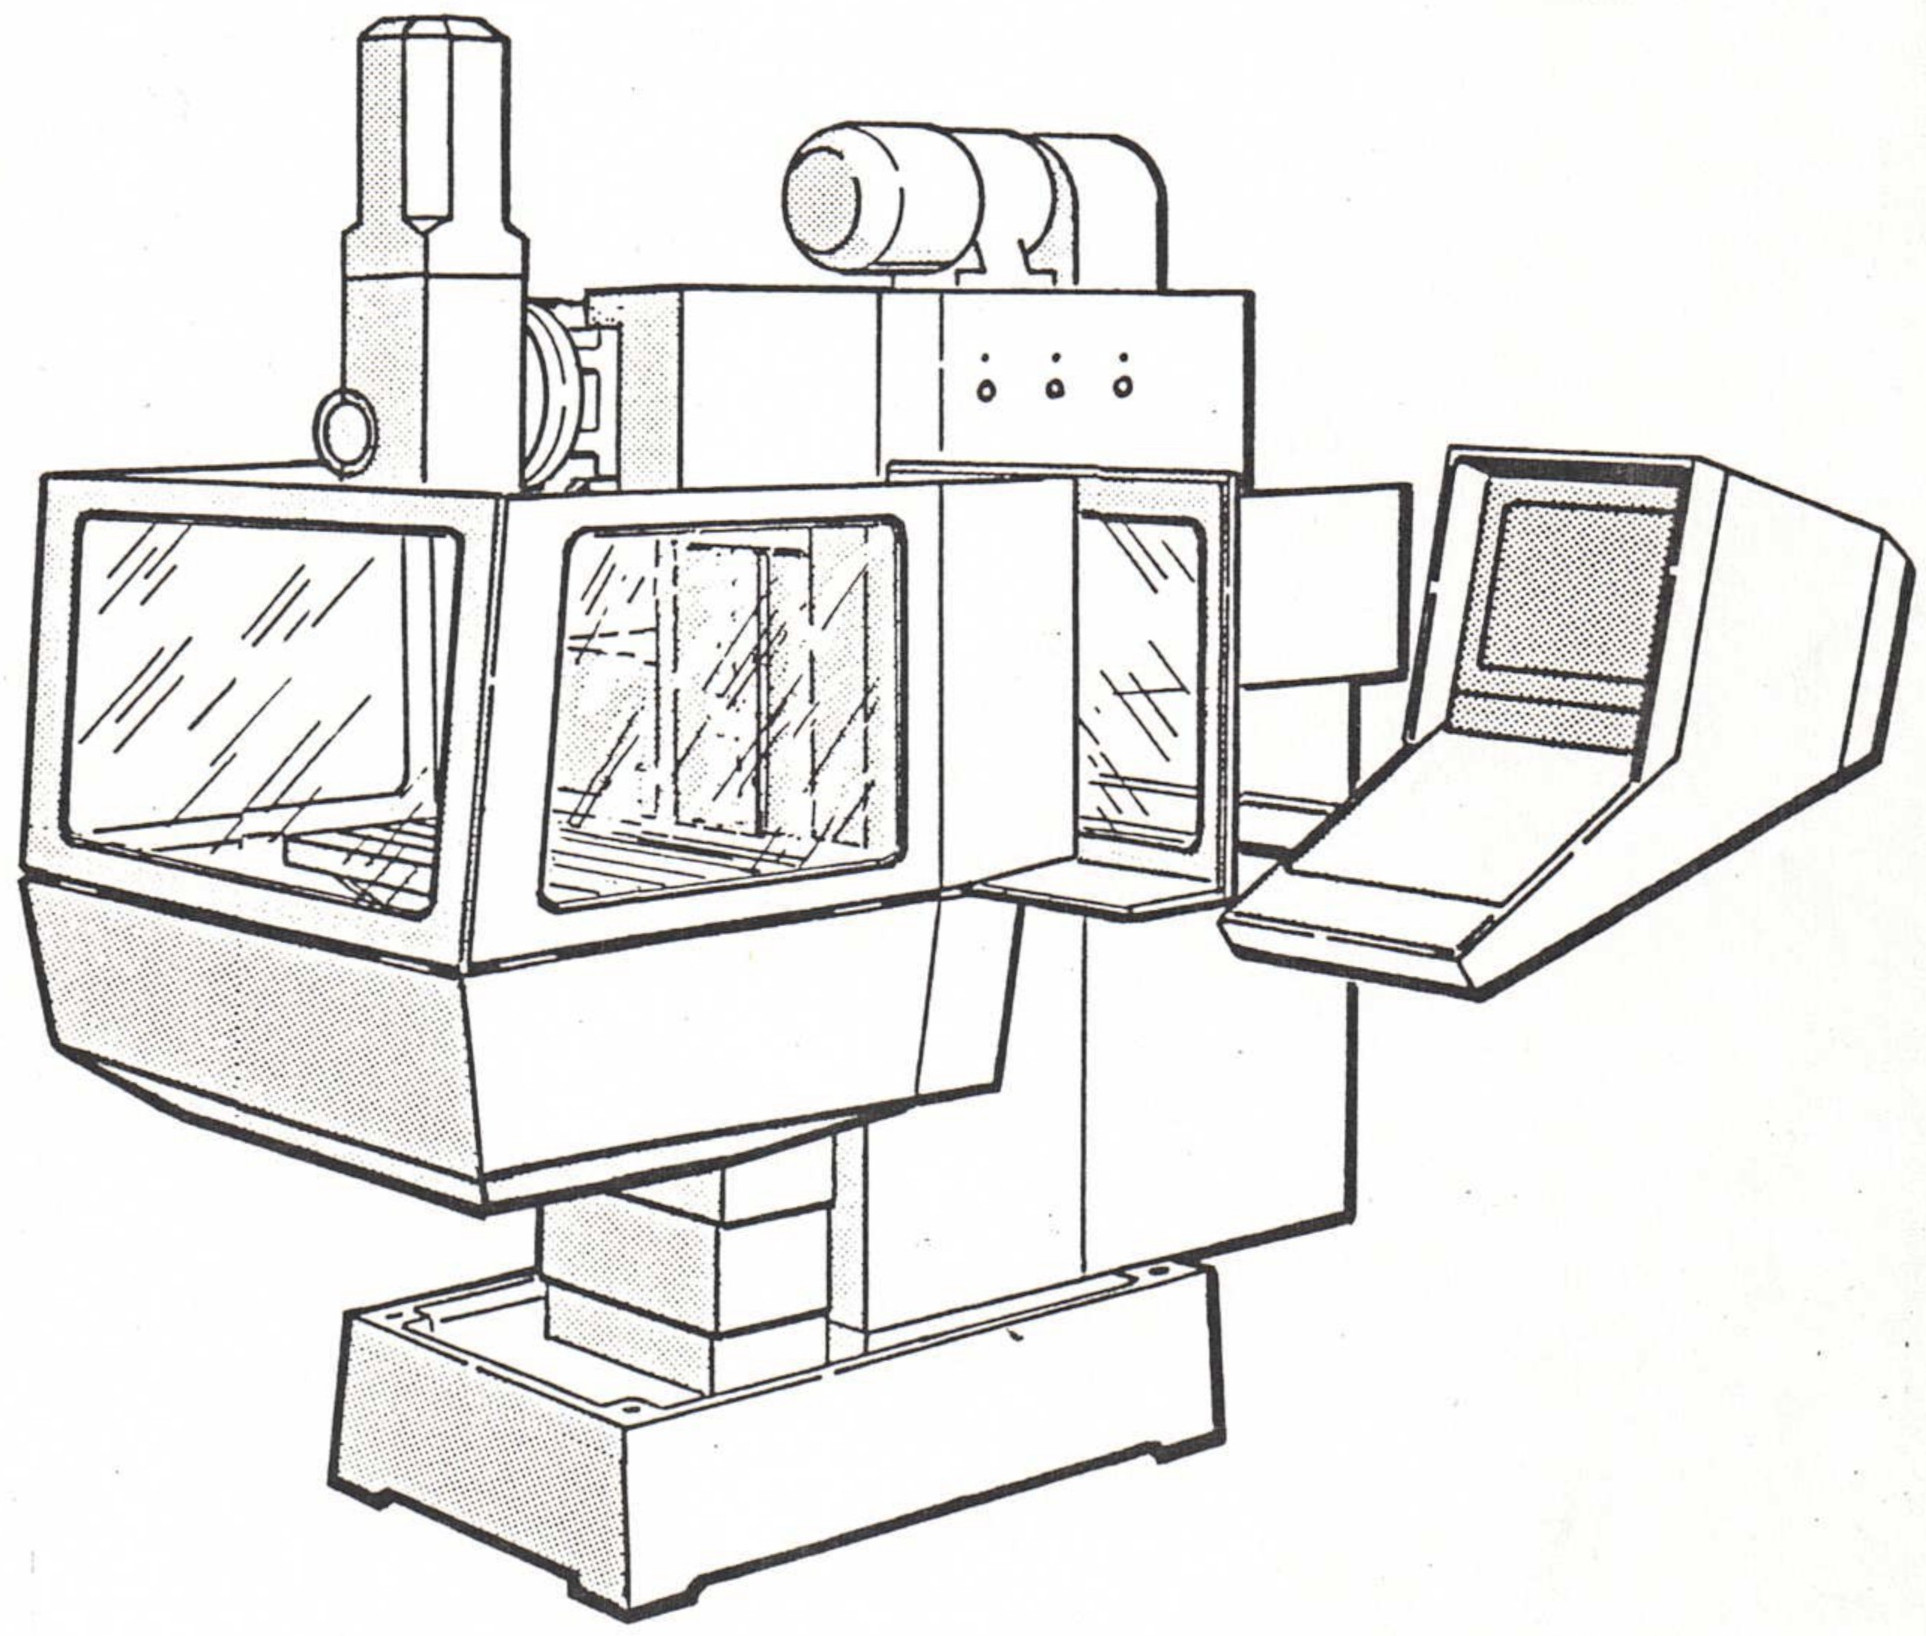
\includegraphics[width=0.9\textwidth]{chapter0/cover-image.jpg} 

        \vfill

         \noindent
         \begin{center}
             \parbox{\textwidth}{\centering {\Huge \textbf{Operation - Maintenance - Repair}}}
         \end{center}
    }
\end{titlepage}

\clearpage % Move to the next page and resume normal styling
\pagestyle{fancy} % Re-enable the default layout

\setsectiontitle{To our customers}
\setcounter{chapter}{0}
\setcounter{section}{0}

This operator's manual contains the essential information required for the proper operation and maintenance of your MAHO machine tool. It belongs in the hands of the operating and maintenance personnel.

The present operator's manual includes the separate operating instructions for CNC 432/10 graphics, the programming instructions for CNC 432 of the control unit, the programming manual for the \enquote{Geometry Package}, and the folder \enquote{Assembly Drawings and Parts Lists}.

Tax-specific details are listed \textbf{only} in the operating manual for CNC 432/10 graphics and should be referenced there.

The machine may only be put into operation after the operating and maintenance personnel have carefully read the operator's manual and have thoroughly\\ familiarized themselves with all details.

Operation and maintenance of the machine must be carried out in accordance with the instructions provided in this operator's manual.

\notebox{NOTE}{\textbf{We assume no liability for damages resulting from failure to follow these instructions or from improper handling.}}

If malfunctions occur that cannot be resolved independently, the cause of the malfunction should be determined using the operator's manual before \\contacting the appropriate MAHO representative or the MAHO company.

This operator's manual is designed to help you complete your machining tasks efficiently. We are confident that the delivered MAHO machine tool will fully meet your expectations. \\[1cm]

\noindent
\textbf{\textcopyright\ Copyright} \\[0.2cm]

This technical manual may \textbf{not}, even in part, be reproduced or made accessible to third parties without the express permission of the publisher.

\newpage

\subsection{Page Numbering}

The pages of this manual are numbered sequentially within each chapter \\according to sections. The page numbers are displayed in the upper right corner and are structured so that the page number follows the section number.

\textbf{EXAMPLE}: \texttt{3.20-3}, means Chapter 3, Section 20, Page 3.

If expansions occur within a section, these are numbered using the page number of the previous page followed by the numbers 1, 2, 3, etc., separated by a period.

\textbf{EXAMPLE}: \texttt{3.20-3.1}, means Chapter 3, Section 20, Page 3, Supplementary Page 1.

Figures and tables are not separately numbered.

The position numbers in the figures refer to the content of the section and can span 2-3 figures.

If positions of a figure are referenced in the text, they are placed within parentheses \texttt{()}.

\subsection{Notices in this Manual}

The following notices are used in this manual:

\notebox{NOTICE}{Applies to technical details that the user must observe.}

\notebox{CAUTION}{Applies to work or operational procedures that must be followed precisely to prevent damage or destruction of the system.}

\notebox{WARNING}{Applies to work or operational procedures that must be followed precisely to prevent hazards to personnel. This also includes \textbf{CAUTION}.}

\subsection{Cross-References}

To avoid redundant descriptions, content-related connections are established in this manual using cross-references.

\textbf{EXAMPLE}:
\begin{quote}
\noindent \hspace{-0.25cm} .... according to instructions .... \\
\hspace{1.3cm} .... see Sheet/Page ....
\end{quote}

\subsection{Location Definition}

The designations front, back, left, right, top, and bottom are based on the perspective from the spindle head looking toward the workpiece.

\setsectiontitle{Table of Contents}
\renewcommand{\arraystretch}{1.3} % Adjust row spacing for readability

\begin{tabularx}{\textwidth}{X r}
    \textbf{\underline{Commissioning the Machine}} & \\ % Main Section (No page number)
    Important Notes \dotfill & 1.01-1 \\
    Transport of the Machine \dotfill & 1.02-1 \\
     & 1.02-2 \\ % No extra &
    Setting Up the Machine \dotfill & 1.03-1 \\
     & 1.03-2 \\
     & 1.03-3 \\
    Setup Plan and Workspace Layout \dotfill & 1.04-1 \\
    Dimensional Drawing of the Machine \dotfill & 1.05-1 \\
    Removal of Rust Protection Agent \dotfill & 1.08-1 \\
    Spindle head oil fill \dotfill & 1.09-1 \\
    Connecting to the Electrical Network \dotfill & 1.10-1 \\
    Commissioning Checklist \dotfill & 1.11-1 \\[0.5cm]

    \textbf{\underline{General Description of the Machine}} & \\ % Main Section
    Technical Data \dotfill & 2.01-1 \\
     & 2.01-2 \\
    Machine Overview \dotfill & 2.02-1 \\
    Component Identification \dotfill & 2.02-2 \\
     & 2.02-3 \\
     & 2.02-4 \\
     & 2.02-5 \\
     & 2.02-6 \\
     & 2.02-7 \\
     & 2.02-8 \\
    Motion Directions \dotfill & 2.03-1 \\
    Control Station \dotfill & 2.04-1 \\
     & 2.04-2 \\
    Hand Control Panel \dotfill & 2.04-5 \\
    Gear Train Schematic \dotfill & 2.10-1 \\
    Main Gearbox \dotfill & 2.10-2 \\[0.5cm]

    \textbf{\underline{Machine Operation}} & \\
    Functional Testing - Trial Run \dotfill & 3.01-1 \\
     & 3.01-2 \\[0.5cm]
\end{tabularx}

\newpage

\begin{tabularx}{\textwidth}{X r}
    Manual Spindle Speed Selection \dotfill & 3.03-2 \\
    Horizontal Working Spindle \dotfill & 3.04-1 \\
    Horizontal Milling with Counter Holder \dotfill & 3.05-1 \\
    Horizontal to Vertical Conversion \dotfill & 3.07-1 \\
    Vertical to Horizontal Conversion \dotfill & 3.08-1 \\
    Vertical Milling Head without Quill Feed \dotfill & 3.09-1 \\
    Automatic Tool Clamping \dotfill & 3.12-1 \\
    Reworking of Standard Tool Shafts \dotfill & 3.13-1 \\
    Tool Shaft According to DIN 69871 \dotfill & 3.13-3 \\
    Manual Adjustment of the Machine Slide \dotfill & 3.15-2 \\
    Hydraulic Plan and Equipment List \dotfill & 3.18-1 \\
    Hydraulic System \dotfill & 3.18-3 \\
    Automatic Central Lubrication System \dotfill & 3.20-1 \\
    Equipment List - Automatic Central Lubrication \dotfill & 3.20-2 \\
    Automatic Central Lubrication \dotfill & 3.20-3 \\
     & 3.20-4 \\
     & 3.20-5 \\
    Coolant System \dotfill & 3.22-1 \\
    Splash Protection \dotfill & 3.24-1 \\[0.5cm]

    \textbf{\underline{Worktables}} & \\
    Fixed Angle Table \dotfill & 4.01-1 \\
     & 4.01-2 \\
    Universal Rotary Table \dotfill & 4.03-1 \\
     & 4.03-2 \\
     & 4.03-3 \\
     & 4.03-4 \\
     & 4.03-5 \\
     Angle Adjustment Display for B-Axis \dotfill & 4.04-1 \\[0.5cm]
\end{tabularx}

\newpage

\begin{tabularx}{\textwidth}{X r}
    \textbf{\underline{CNC Control}} & \\ % Main Section (No page number)
    Linear Measurement Systems and Display Units \dotfill & 5.01-1 \\
    Machine Constants CNC 432 \dotfill & E3.21741C \\
     & E3.21742C \\
     & E3.21743C \\
     & E3.21744C \\
     & E3.24628C \\
     & E3.24629C \\
     & E3.24630C \\
    Error List CNC 432 \dotfill & E3.22870C \\
     & E3.22871C \\
     & E3.22872C \\
     & E3.25024C \\
    Operating Manual CNC 432/Graphics \dotfill & 76.00471 \\
    Geometry Package for CNC 432/Graphics \dotfill & 76.00461 \\
    Programming Manual CNC 432 \dotfill & 76.00211 \\[0.5cm]

    \textbf{\underline{Accessories}} & \\ % Main Section
    High-Speed Milling Spindle \dotfill & 6.02-1 \\
    Dot-Matrix Printer ZIP 30 (Separate Manual) \\[0.5cm] % No page number

    \textbf{\underline{Maintenance}} & \\ % Main Section
    Important Notes \dotfill & 7.01-1 \\
    Machine Lubrication Plan \dotfill & 7.02-1 \\
    Lubrication Schedule \dotfill & 7.03-1 \\
    Lubricant Recommendations \dotfill & 7.06-1 \\
     & 7.06-2 \\
    Coolants \dotfill & 7.07-1 \\
     & 7.07-2 \\
     & 7.07-3 \\
     & 7.07-4 \\[0.5cm]
\end{tabularx}

\newpage

\begin{tabularx}{\textwidth}{X r}
    Removing the Machine Covers \dotfill & 7.10-1 \\
    Maintenance Plan \dotfill & 7.20-1 \\
    Overview of Maintenance Tasks for Mechanics and Hydraulics \dotfill & 7.21-1 \\
    Overview of Maintenance Tasks for Electrical and Electronics \dotfill & 7.22-1 \\
    Special Tools for Maintenance and Servicing \dotfill & 7.23-1 \\
    Adjusting the Gibs \dotfill & 7.30-1 \\
    Guideway Wiper Maintenance \dotfill & 7.31-1 \\
    Replacing the Feed Drive Timing Belt \dotfill & 7.33-1 \\
     & 7.33-2 \\
     & 7.33-3 \\
     & 7.33-5 \\
    Installation and Maintenance of the Poly-V Belt \dotfill & 7.34-1 \\
     & 7.34-2 \\
    Adjusting the Collet for Automatic Tool Clamping \dotfill & 7.35-1 \\
     & 7.35-2 \\
    Readjustment Work on the Universal Rotary Table \dotfill & 7.40-1 \\
     & 7.40-2 \\
    Maintenance of DC Motors \dotfill & 7.60-1 \\
     & 7.60-2 \\
     & 7.60-3 \\
    Maintenance of Three-Phase Motors \dotfill & 7.61-1 \\[0.5cm]

    \textbf{\underline{Spare Parts Plans and Lists}} & \\ % Main Section
    Notes on Ordering Spare Parts \dotfill & 8.00-1 \\
    Spare and Wear Parts List \dotfill & 99.34504 \\[0.5cm]

    \textbf{\underline{Disassembly Instructions}} & \\ % Main Section
    Main Motor \dotfill & 9.01-1 \\
    Replacing the Feed Motor \dotfill & 9.08-1 \\
     & 9.08-2 \\
     & 9.08-3 \\
\end{tabularx}

\notebox{NOTE}{The mandatory machine constants for the machine are supplied as punched tape and plaintext. They are located with the electrical circuit diagrams in the control cabinet of the machine.}

\refstepcounter{chapter}
\addcontentsline{toc}{chapter}{Before Starting the Machine}

\section{Important Notes}

\subsection{Factory Number}
\begin{itemize}
    \item The information in this operator's manual applies \uline{\textbf{only}} to the machine whose factory number is stamped on the machine's nameplate.
    \item For all inquiries and spare part orders, the factory number of the machine must be specified.
    \item If inquiries pertain to a specific page of the operator's manual, the page number must also be provided.
\end{itemize}

\subsection{Before Starting the Machine}
\begin{itemize}
    \item Carefully read the operator's manual.
    \item Set up the machine (see Page 1.03-1).
    \item Ensure that the machine has reached room temperature.
    \item Remove rust protection (see Page 1.08-1).
    \item Tighten all terminal screws on the terminal strips, contactors, relays, and fuses in the control cabinet; they may have loosened due to vibrations during transport.
    \item Connect the machine to the electrical network (see Page 1.10-1).
    \item Check oil levels (see Page 7.02-1 and 7.03-1).
    \item Fill the machine with coolant (see Page 3.22-1).
\end{itemize}

\subsection{Interlocks of the Machine}
\begin{itemize}
    \item After switching off the main switch -Q1- in the control cabinet and after every power failure, the machine must be restarted.\footnotemark[1]
    \item The red mushroom button of the EMERGENCY STOP switch must not be pressed during this process.
    \item After each EMERGENCY STOP, the corresponding mushroom button must be \\released by turning it clockwise, and the machine must be restarted.\textsuperscript{\footnotemark[1]}
\end{itemize}

\footnotetext[1]{"Start the machine", see separate CNC 432 operating instructions.}

\section{Transport of the Machine}

The dimensions and weights of the machine with the fixed table and coolant container are as follows:

\begin{table}[h]
\centering
\begin{tabular}{lll}
\textbf{Packaging Type} & \makecell{\textbf{Dimensions}\\\textbf{(L x W x H) [m]}} & \textbf{Weight [kg]} \\ \hline
EURO Packaging (Pallet/Carton) & $1.9 \times 1.8 \times 2$ & 1450 \\
Box (USSR) & $1.9 \times 1.9 \times 2.05$ & 1590 \\
Box (Seaworthy) & $2.35 \times 1.9 \times 2.05$ & 1693 \\
Container Loading (Machine on Pallet) & $1.8 \times 1.8 \times 1.98$ & 1362 \\
\end{tabular}
\end{table}

\begin{figure}[h]
    \centering
    \begin{minipage}[b]{0.35\textwidth} % Align to the bottom with [b]
        \centering
        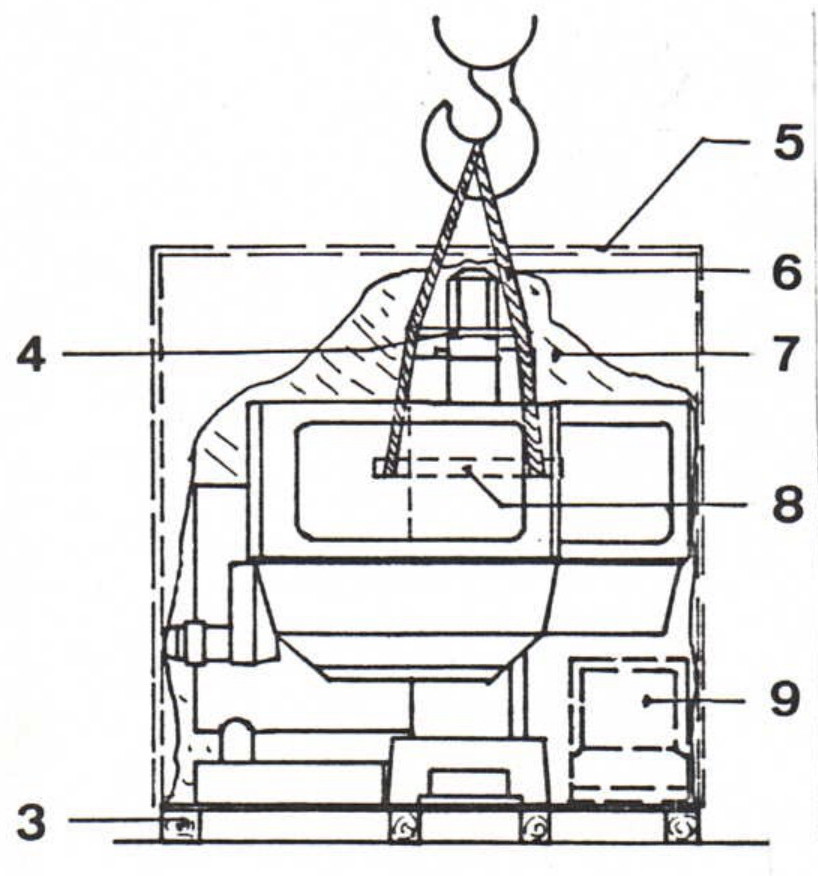
\includegraphics[width=\textwidth]{chapter1/machine_packaging_transport.jpg} % Replace with actual image file
        \caption{}
        \label{fig:packaging}
    \end{minipage}
    \hfill
    \begin{minipage}[b]{0.55\textwidth} % Align to the bottom with [b]
        \centering
        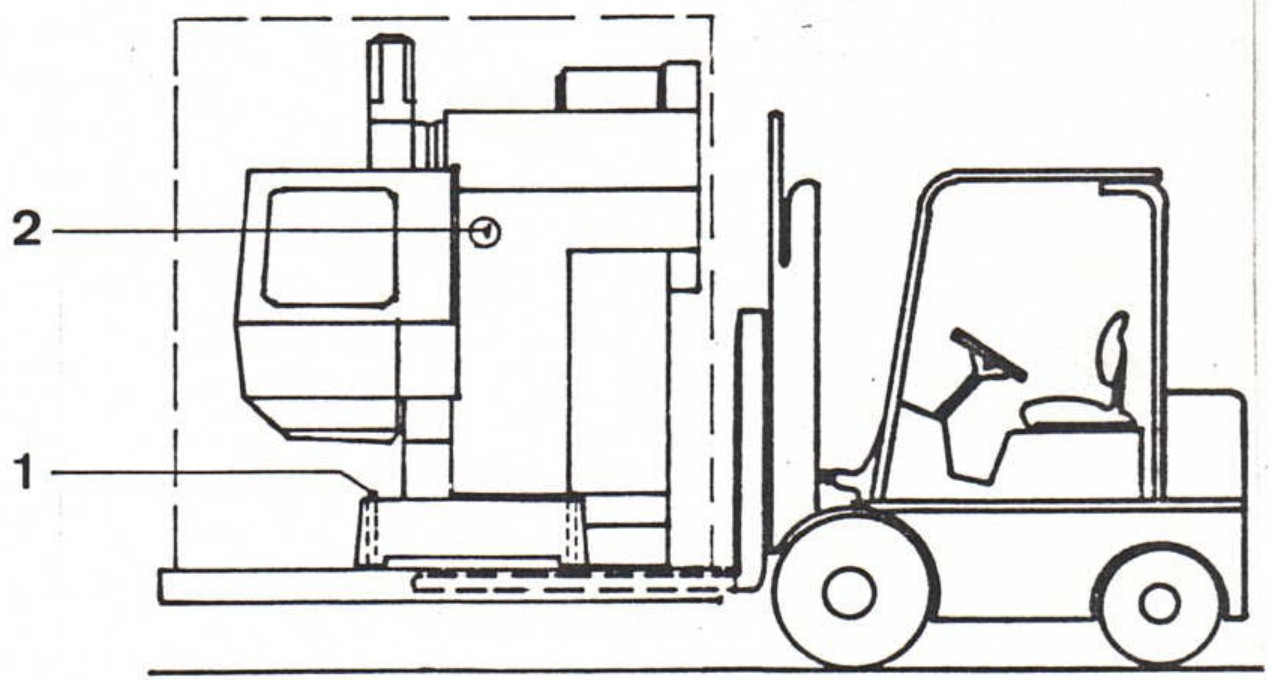
\includegraphics[width=\textwidth]{chapter1/machine_unloading_forklift.jpg} % Replace with actual image file
        \caption{}
        \label{fig:unloading}
    \end{minipage}
\end{figure}

\begin{itemize}
    \item Unload the packaged machine from the transport device using a forklift, hoist, or similar equipment.
    \item Remove the packaging (\textbf{5}) and cut and remove the protective foil (\textbf{7}) from the base of the box. Take off the sealing covers (\textbf{2}) on both sides.
    \item Check the machine and accessories for any transport damage.
\end{itemize}

\notebox{NOTE}{Damages or other defects, such as incompleteness, must be reported immediately in writing to the shipping company or railway, the insurance company, and the company MAHO.} 

\begin{itemize}
    \item Insert the transport rod (\textbf{8}) (maximum 50 mm diameter, 1000 mm length) into the opening in the stand.
    \item Attach the endless sling (\textbf{6}), with a minimum load capacity of 3000 kg and a total length of approximately 6 m, to the crane hook and the transport rod.
\end{itemize}

\notebox{CAUTION}{Place the detached control panel (\textbf{9}) on the work table and secure it against slipping!}

\sectionLikeSubsection{Transport of the Machine}

\begin{itemize}
    \item Perform a hanging test, i.e., align the machine by moving the transport rod (\textbf{8}) in the stand so that it hangs horizontally. Using a spacer (\textbf{4}) prevents the rope from rubbing against the machine.
    
    \item Lower the machine, unscrew the fastening nuts (\textbf{1}), and remove the pallet or box bottom (\textbf{3}) after lifting the machine again.
\end{itemize}

\textbf{When using a forklift:} Place the machine on wooden boards laid on the forks of the forklift (Fig. \ref{fig:unloading}) or hang it on the forks using a rope (Fig. \ref{fig:machine_placement_forklift}).
    
In unfavorable space conditions, use the "Transport Mule" (Fig. \ref{fig:machine_placement_mule}).

\begin{itemize}
    \item Transport the machine to the prepared location according to Page 1.03-1 and carefully place it on the damping plates provided.
\end{itemize}

\begin{figure}[h]
\centering
\begin{minipage}[t]{0.45\textwidth}
    \centering
    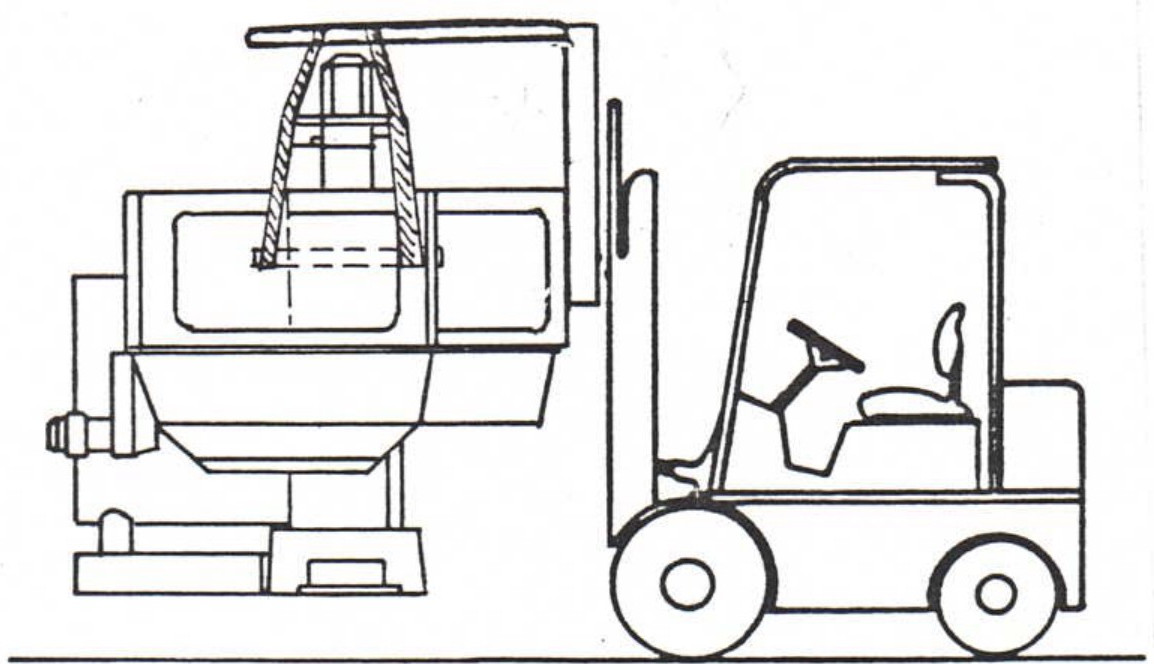
\includegraphics[width=\textwidth]{chapter1/machine_placement_forklift.jpg} % Replace with actual image file
    \caption{}
    \label{fig:machine_placement_forklift}
\end{minipage}
\hfill
\begin{minipage}[t]{0.45\textwidth}
    \centering
    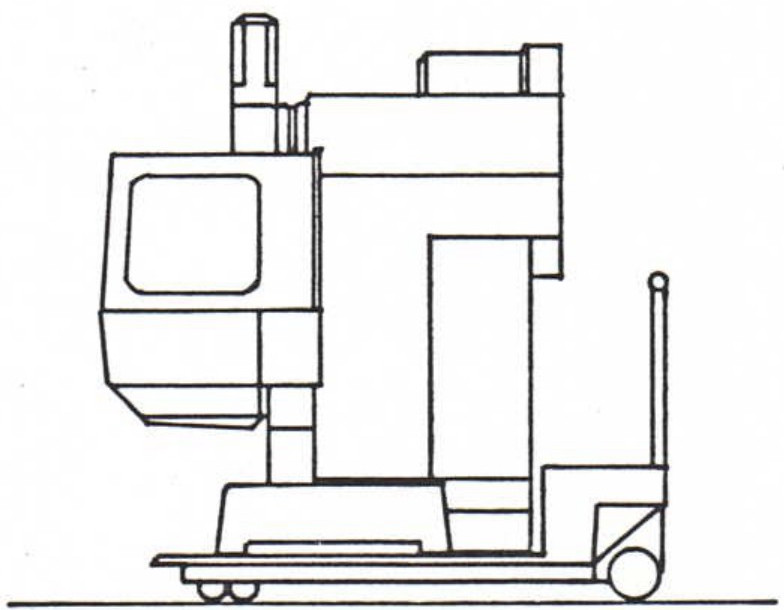
\includegraphics[width=\textwidth]{chapter1/machine_placement_mule.jpg} % Replace with actual image file
    \caption{}
    \label{fig:machine_placement_mule}
\end{minipage}
\end{figure}

\vspace{1em}

\infoBullet{Setup plan and workspace layout}{1.04-1}

\section{Installation of the Machine}

\subsection{Installation Site}
To ensure proper functionality of the machine, the following points regarding the installation site must be observed:
\begin{itemize}
    \item It must be free from vibrations.
    \item It must be free from local, one-sided heating or cooling of the machine, e.g., sunlight, radiators, drafts, etc.
    \item It must be free from interfering electrical installations (high-frequency).
    \item The total floor area requirement ($A_\text{WMP}$) is $3.2 \times 3.4 \, \text{m}$ ($10.88 \, \text{m}^2$).
    \item Within this total area, the machine covers an area of $3.5 \, \text{m}^2$, for which a minimum load-bearing capacity of $400 \, \text{daN/m}^2 \, (0.40 \, \text{t/m}^2)$ must be ensured.
    \item Ideally, the floor should be concrete or wood block.
\end{itemize}

\notebox{CAUTION}{
Mixed floors, i.e., machine standing on both concrete and wood block, are not permissible.
}

\begin{itemize}
    \item The unevenness of the floor must not exceed $3 \, \text{mm/m}^2$.
    \item A constant room temperature of max. $30^\circ \text{C}$ ($303 \, \text{K}$) must not be exceeded.
    \item The relative humidity must not exceed $80\%$.
\end{itemize}

\notebox{NOTE}{
Higher humidity or room temperatures up to $55^\circ \text{C}$ ($328 \, \text{K}$) are permissible when using MAHO cooling units in the command station and control cabinet.
}

\infoBullet{Setup plan and workspace layout}{1.04-1}\\
\infoBullet{Dimensions of the machine}{1.05-1}

\newpage
\sectionLikeSubsection{Setup of the Machine}

\begin{itemize}
    \item Lay out the supplied \enquote{Airlock damping plates} (1) according to the following sketch.
    \item Carefully place the machine on the damping plates.
    \item Leveling in the Z-direction (using shims) is necessary to ensure the oil level in the spindle head is maintained accurately!
    \item Position the coolant tank (2) accordingly, and screw the coolant pump (3) and return line (5) into the tank lid (4).
\end{itemize}

\vspace{1cm}

\begin{figure}[h!]
    \centering
    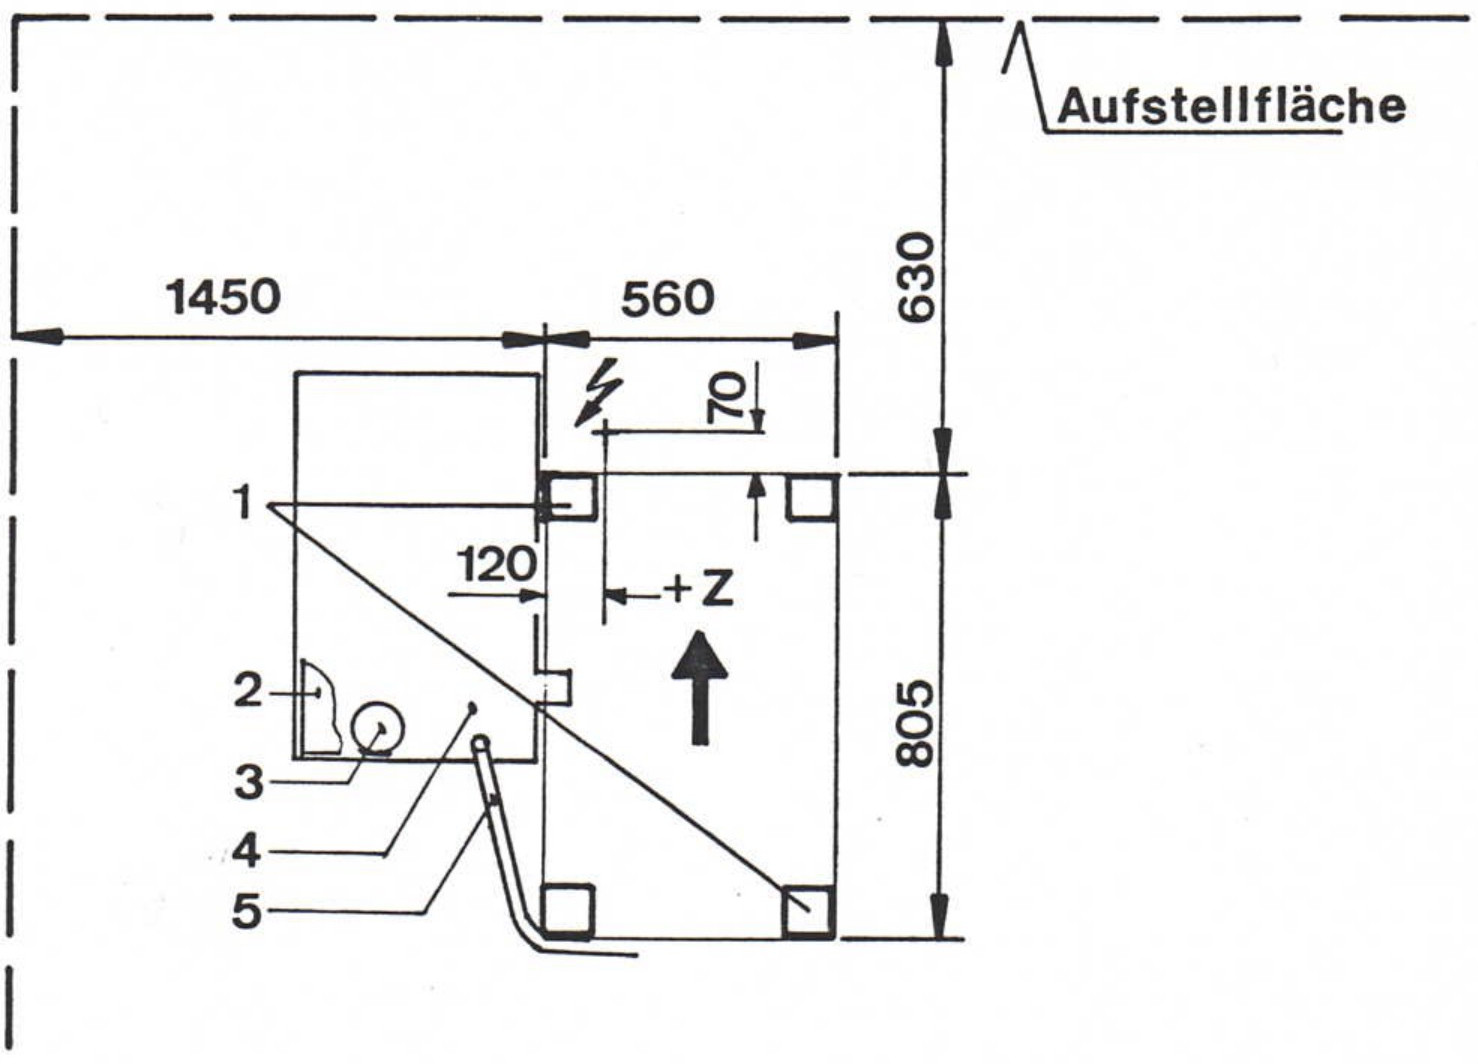
\includegraphics[width=\textwidth]{chapter1/machine_setup_sketch.jpg}
    \caption{Sketch for machine setup, including leveling and coolant system placement.}
    \label{fig:machine_setup_sketch}
\end{figure}

\sectionLikeSubsection{Mounting the Control Panel}

\begin{itemize}
    \item Remove the cover (7) and, if necessary, (9).
    \item Pull the pivot pin (8) out of the support (14).
    \item Place the extension arm (11) onto the support (14), slide the fork end \\(11.1) over the stop screw (12), and insert the cable bundle (13) into the bottom opening of the extension arm (11).
    \item Insert the pivot pin (8) into the extension arm (11) and the support (14). Tighten the mounting bracket of the cable hose (15) \\onto the extension arm.
    \item Insert the control panel (5) into the extension arm (11).
\end{itemize}

\begin{figure}[h!]
    \centering
    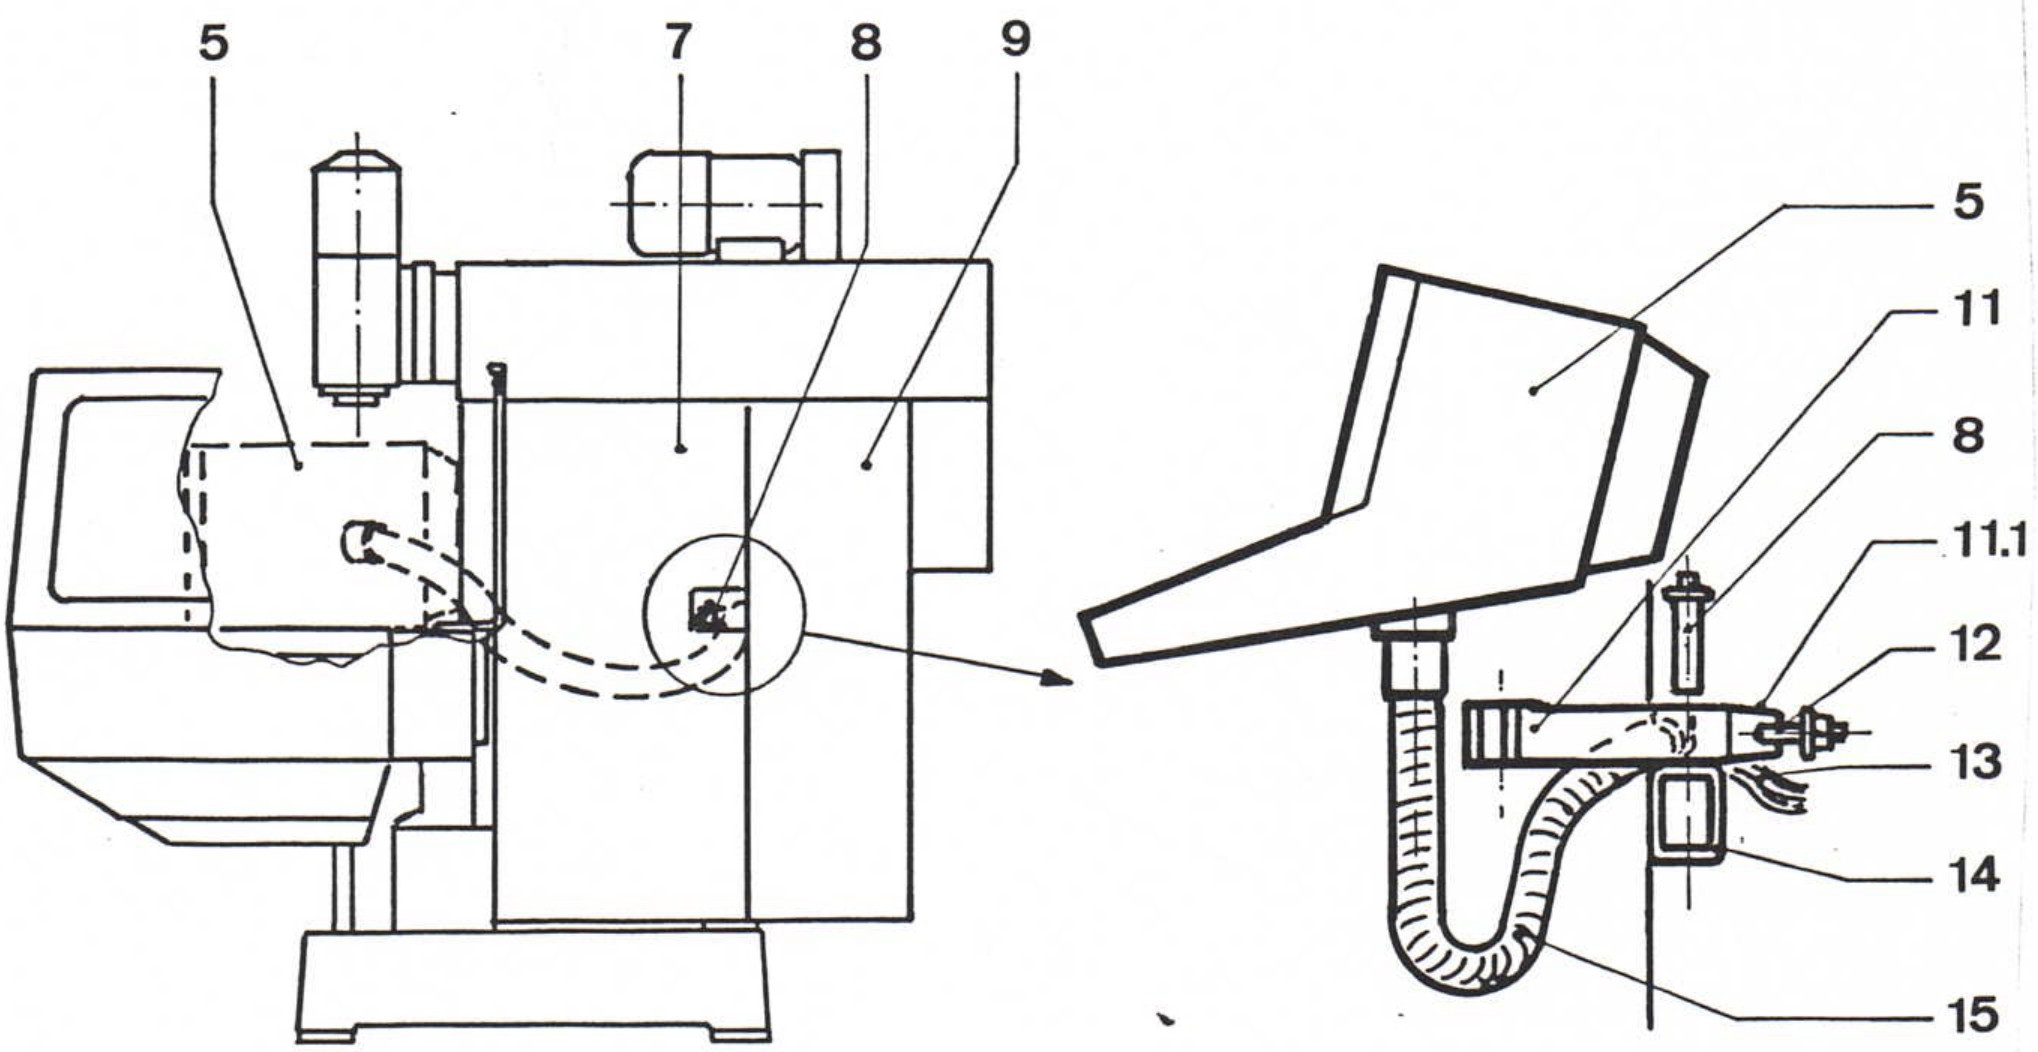
\includegraphics[width=\textwidth]{chapter1/control_panel_mounting_diagram.jpg}
    \caption{}
    \label{fig:control_panel_mounting}
\end{figure}

\section{Setup Plan and Workspace Layout}

\begin{description}[labelwidth=4cm, labelindent=0cm, leftmargin=0cm, rightmargin=2cm]
    \item[Total space requirement:] \dotfill 10.5 m\textsuperscript{2}
    \begin{itemize}
        \item Area for maintenance and disassembly \dotfill 5.06 m\textsuperscript{2}
        \item Machine footprint \dotfill 0.42 m\textsuperscript{2}
        \item Operator space \dotfill 3.8 m\textsuperscript{2}
        \item Setup area \dotfill 1.6 m\textsuperscript{2}
        \item Coverage area (F) \dotfill 3.25 m\textsuperscript{2}
    \end{itemize}
    \item[Height of the machine:] \dotfill 1.83 m
    \item[Weight of the machine (total):] \dotfill approx. 1,250 kg
    \item[Floor load on area (F):] \dotfill approx. 400 kg/m\textsuperscript{2}
\end{description}

\begin{figure}[H]
    \centering
    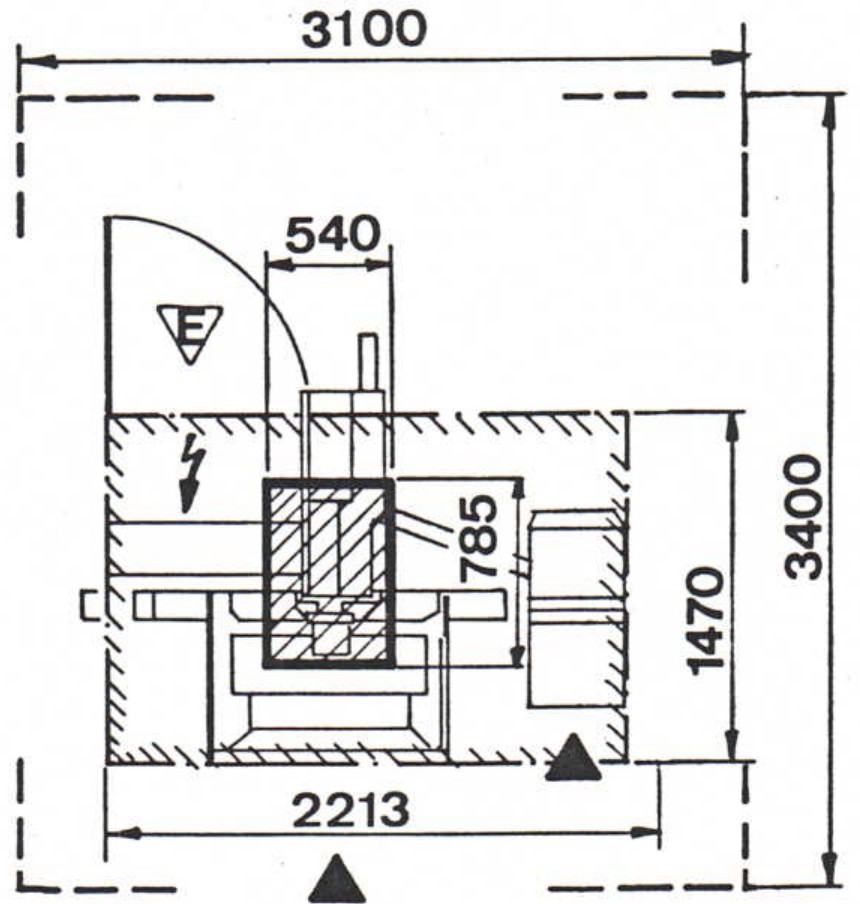
\includegraphics[width=0.45\textwidth]{chapter1/setup_plan_workspace_layout_diagram.jpg}
    \caption{}
    \label{fig:setup_plan_workspace_layout}
\end{figure}

\begin{description}[labelwidth=0cm, labelindent=0cm, leftmargin=0cm]
    \item \adjustbox{valign=c}{
\includegraphics[height=1cm]{chapter1/icon_electrician_access.jpg}} \hspace{0.5cm} Electrician access
    \item \adjustbox{valign=c}{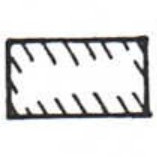
\includegraphics[height=1cm]{chapter1/icon_coverage_area.jpg}} \hspace{0.5cm} Coverage area (F)
    \item \adjustbox{valign=c}{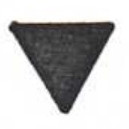
\includegraphics[height=1cm]{chapter1/icon_operator_position.jpg}} \hspace{0.5cm} Operator position
\end{description}

\vspace{-\topsep} % Suppress extra vertical space above the block
\begin{minipage}{\textwidth}
    \begin{minipage}[t]{1.5cm} % Adjust the width for the icon
        \raggedright
        \raisebox{-0.5\height}{% Adjust vertical alignment of the icon
            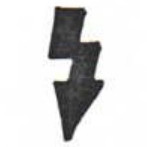
\includegraphics[height=1cm]{chapter1/icon_electrical_connection.jpg}
        }
    \end{minipage}%
    \begin{minipage}[t]{\dimexpr\textwidth-1.5cm\relax} % Remaining space for text
        \begin{description}[labelwidth=6cm, labelindent=0cm, leftmargin=7cm, itemsep=0pt]
            \item[Power connection:] \dotfill 11 kVA
            \item[Free cable length across the floor:] \dotfill 0.5 m
            \item[Maximum fuse rating:] 
            \begin{itemize}[itemsep=0pt, topsep=0pt]
                \item 200-220 V \dotfill 35 A
                \item 380-500 V \dotfill 25 A
            \end{itemize}
        \end{description}
    \end{minipage}
\end{minipage}

\section{Dimensional Drawing of the Machine}

\begin{figure}[H]
    \centering
    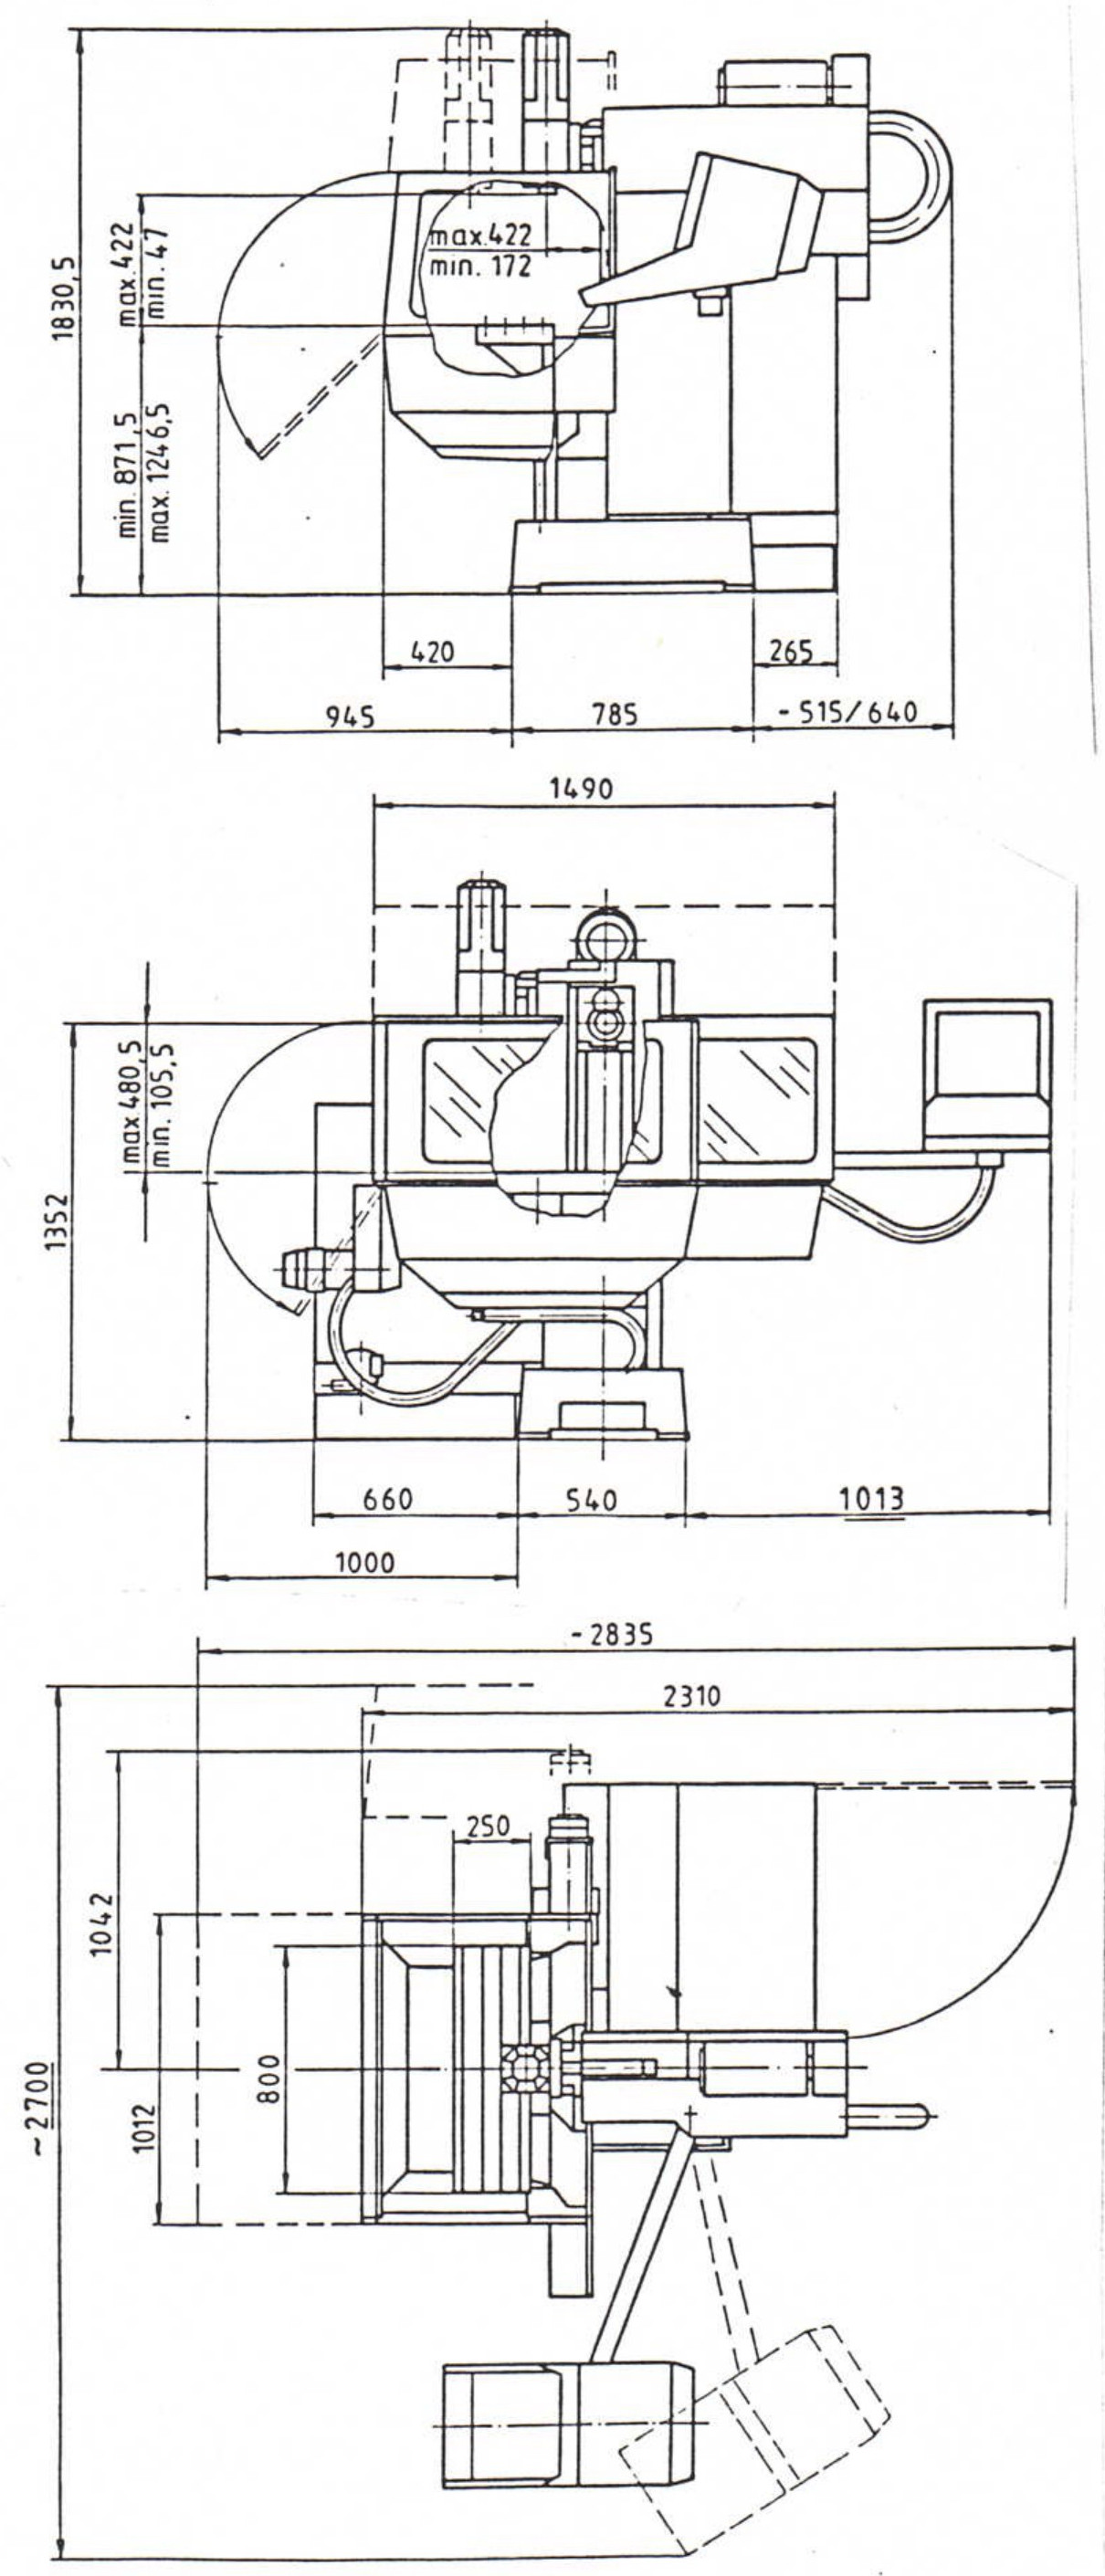
\includegraphics[width=.55\textwidth]{chapter1/machine_dimensions.jpg}
    \caption{}
    \label{fig:setup_plan_workspace_layout}
\end{figure}


\section{Removal of the Rust Protection Agent}

\setcounter{section}{8}

\notebox{WARNING}{Before removing the rust protection agent from the machine, no adjustments to the slides must be made.}

\begin{figure}[h]
    \centering
    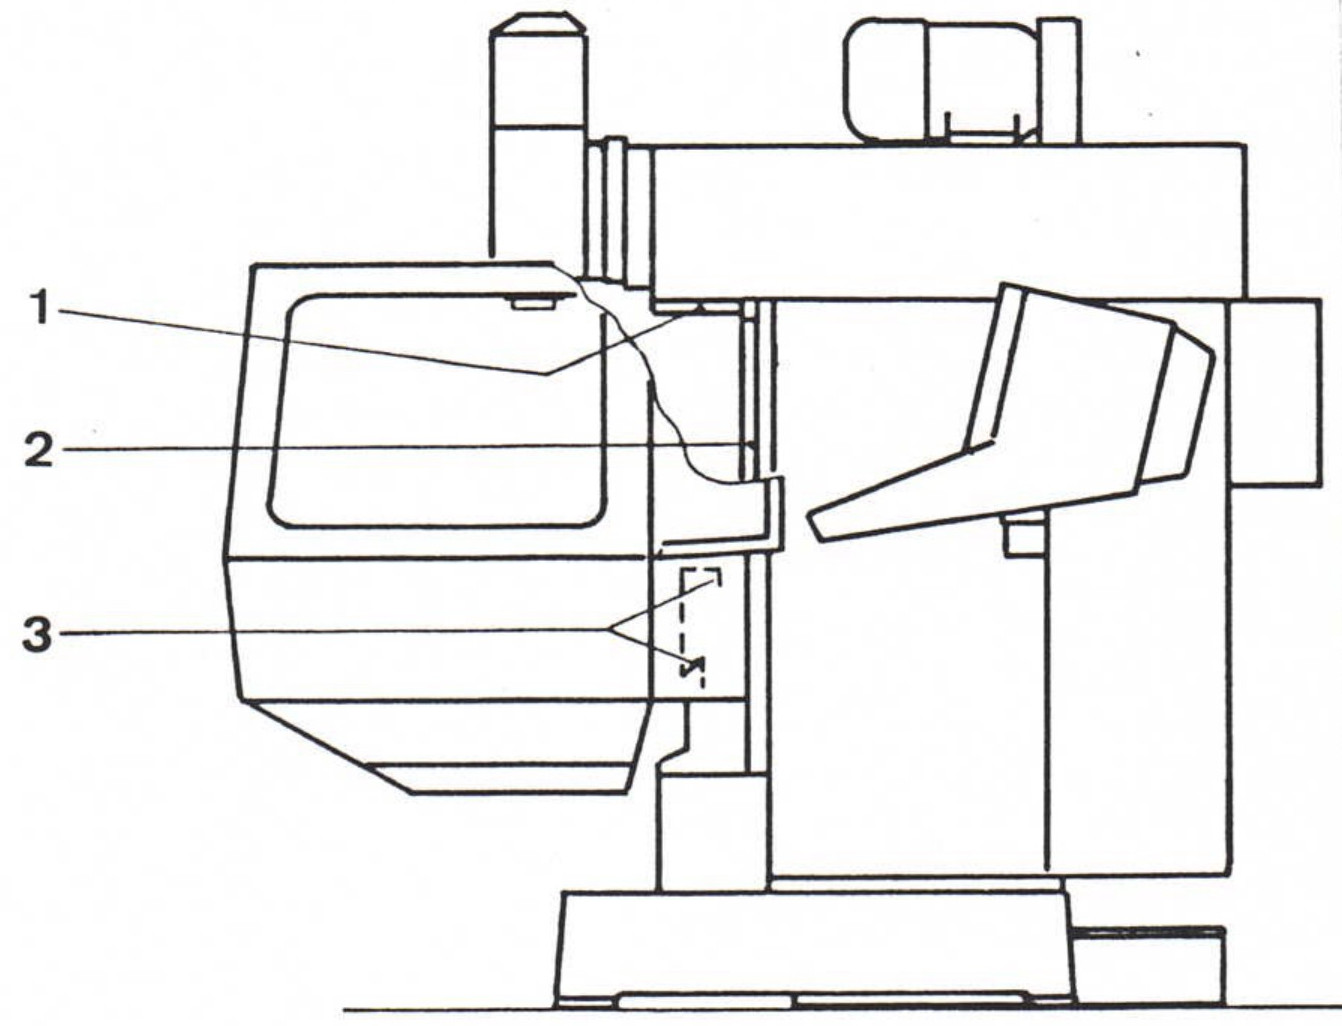
\includegraphics[width=0.7\textwidth]{chapter1/diagram_removal_of_rust_protection_agent.jpg}
    \caption{}
\end{figure}

\begin{itemize}
    \item Carefully remove the rust protection agent from the bare external surfaces and the receptacle cones of the work spindles using a soft cloth soaked with petroleum, gasoline, tetra, or another solvent for hydrocarbons.
    \item \textbf{Do not under any circumstances use scrapers or other sharp tools for this task.}
    \item Clean the sliding surfaces of the dovetail guides of the headstock (1) and the cross slide (2) with a soft cloth to remove the rust protection grease and apply oil with a brush.\footnotemark[2]
    \item Clean accessible sliding surfaces of the combined dovetail flat guides (3) of the vertical clamping table with a soft cloth to remove the rust\\ protection grease and apply oil.
\end{itemize}

\footnotetext[2]{The oil used in the central lubrication system must be applied (see page 7.06-1 \enquote{Lubricant Recommendations}).}

\notebox{WARNING}{Mixing of oils must be strictly avoided.}

\section{Filling the Drive Gear Oil Reservoir in the Spindle Head}

To prepare the machine for operation, the oil in the work spindle drive must be drained during transport and refilled before commissioning.

\vspace{.5cm}

\notebox{CAUTION}{Verify that the machine is level in the Z-axis using a spirit level, and adjust if necessary.\footnotemark[3]}

\footnotetext[3]{See Sheet 1.03-1.}

\begin{itemize}[itemsep=0.5em]
    \item Unscrew the front fill screw (1).
    \item Using the supplied container labeled "CLP 46/HLP 46" (Aral Sumorol CM 46), pour 0.2 liters into a measuring container and fill it into the fill opening (2) on the spindle head.
    \item Wait approximately 10 minutes, then read the oil level in the sight glass. If necessary, refill the remaining quantity in steps of 0.1 liters using the measuring container until the oil level reaches the corresponding mark (3).
    \item Reattach the fill screw (1).
\end{itemize}

\begin{figure}[h!]
    \centering
    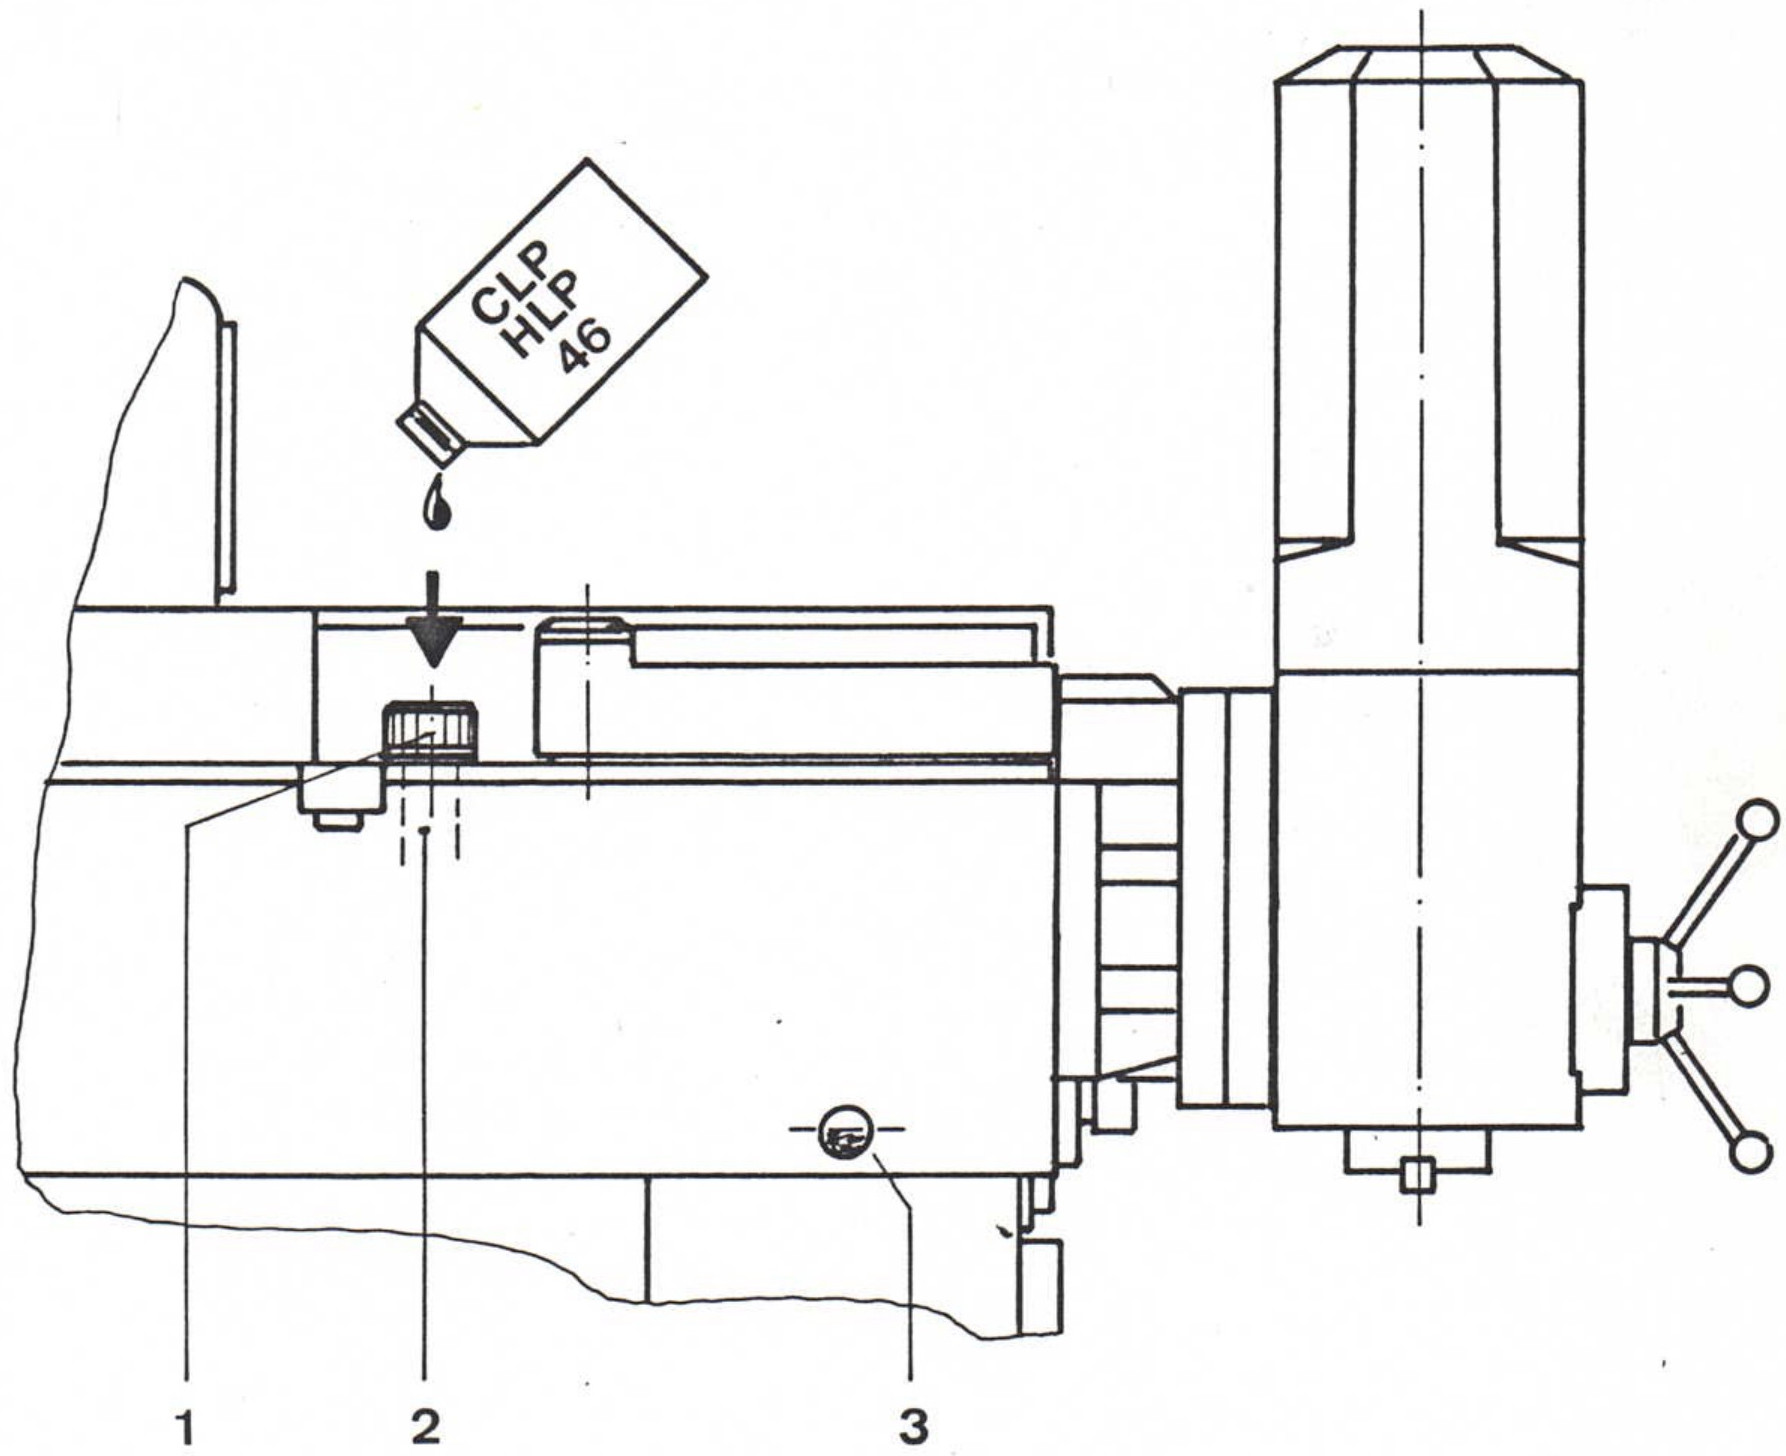
\includegraphics[width=0.8\textwidth]{chapter1/spindle_oil_fill_diagram.jpg} % Replace with your image filename
    \caption{}
\end{figure}


\section{Connecting to the Electrical Network}

Connection regulations from the responsible power supply company must be observed.

\begin{figure}[htp] % Top alignment for the figure
    \centering
    \begin{minipage}[t]{.4\linewidth} % Adjust the width for the image
        \centering
        \raisebox{-\height}{% Top-align the image
            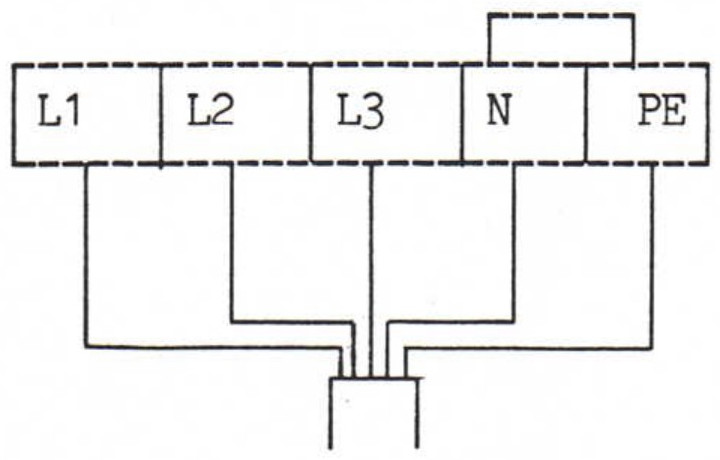
\includegraphics[width=\linewidth]{chapter1/electrical_connection_diagram.jpg}
        }
        \caption{Electrical connection diagram.} % Caption below the image
        \label{fig:electrical_connection} % Optional: add label for referencing
    \end{minipage}%
    \hfill % Add space between image and text
    \begin{minipage}[t]{\dimexpr\textwidth-8cm\relax} % Remaining width for the text
        \vspace{0pt} % Ensures top alignment of this minipage
        Total connection power: \dotfill 11 kVA \\\\
        Fuse, max.: \\
        200-220 V \dotfill 35 A \\
        380-500 V \dotfill 25 A
    \end{minipage}
\end{figure}

\begin{itemize}
    \item Switch off the main switch \textbf{-Q1-} on the control cabinet.
    \item Open the control cabinet door. Feed the connection cable through the \\provided opening and connect it to the input terminals L1, L2, L3, N, PE.
    \item For 4-pole connections, terminals N and PE must be bridged.
    \item Check the phase sequence using a phase sequence indicator on terminals L1, L2, L3. If necessary, swap two phases at the input terminals.
    \item Check all terminal screws on the terminal strips, contactors, relays, and fuses in the control cabinet for tightness.
    \item Only after establishing the correct phase sequence, switch on the main \\switch \textbf{-Q1-} on the control cabinet and perform a function test following the instructions on Page 3.01-1.
\end{itemize}

\notebox{NOTE}{The electrical documentation is located in a pocket on the inside of the control cabinet door and must remain in the machine!}

\notebox{CAUTION}{When connecting peripheral devices (reader-puncher, corner milling head, grinding head), check the voltage of the socket.}

Fuses must only be replaced with equivalent types.

Adjustment values on potentiometers, adjustment switches, machine parameters, etc., must only be changed by service personnel.

\section*{Commissioning Checklist}

Before starting the working spindles and axis movements, the following points must be completed:

\begin{enumerate}
    \item Proper setup, see page 1.03-1.
    \item Rust protection removed, see page 1.08-1.
    \item Oil bath filled, see page 1.09-1.
    \item Electrical connection, see page 1.10-1.
\end{enumerate}
\refstepcounter{chapter}
\addcontentsline{toc}{chapter}{General Description of the Machine}

\section{Technical Data}

\subsection{Work Area}
Adjustment of the cross support:
\begin{itemize}
    \item in the horizontal longitudinal axis (X-axis): \dotfill 400 mm
    \item in the vertical axis (Y-axis): \dotfill 375 mm
\end{itemize}

\noindent Adjustment of the spindle head:
\begin{itemize}
    \item in the horizontal transverse axis (Z-axis): \dotfill 250 mm
\end{itemize}

\subsection{Workspace}
Vertical mounting table \footnotemark[4]
\begin{itemize}
    \item Clamping surface: \dotfill 510 x 800 mm
    \item Number of guide grooves: \dotfill 1
\end{itemize}

\footnotetext[4]{Worktables, see Section 4 of the technical documentation.}

\subsection{Working Spindles}
\begin{itemize}
    \item Tool holder:\footnotemark[5] \dotfill ISO 40
    \item Quill stroke of the vertical working spindle: \dotfill 50 mm
    \item Clamping force of the tool clamp ISO-Type B Clamping pin: \dotfill N \footnotemark[6]
    \item MAHO-OTT Clamping groove: \dotfill N \footnotemark[6]
\end{itemize}

\footnotetext[5]{For tool holding according to DIN 69871, with pull studs ISO 7388, Type B.}
\footnotetext[6]{Tool clamping, see sheet 3.12-1; tool holders, see sheets 3.13-1 and 3.13-3.}

\subsection{Speeds and Feeds}
Working spindle speeds,\footnotemark[7] \\Directly programmable: \dotfill 80 - 4000 rpm

\footnotetext[7]{Transmission with 18 speed levels and a manual shifting step of 1.25, controlled by CNC and manually switchable.}

\vspace{.5cm}
\noindent Feeds, directly programmable: \footnotemark[8]
\begin{itemize}
    \item In the X, Y, Z axes: \dotfill 0.1 - 1500 mm/min
\end{itemize}

\footnotetext[8]{Minimum feed rate in axes X, Y, Z: 1 mm/min.}

\vspace{.2cm}
\noindent Rapid traverse:
\begin{itemize}
    \item In the X, Y, Z axes: \dotfill 2.5 m/min
\end{itemize}

\newpage
\subsection{Electrical Equipment}
\begin{itemize}
    \item Voltage: \dotfill 220/380 V \footnotemark[9]
    \item Frequency: \dotfill 50/60 Hz \footnotemark[9]
    \item Total connected load of the machine: \dotfill 11 kVA \footnotemark[9]
\end{itemize}

\footnotetext[9]{Standard configuration.}

\subsection{CNC Control\textsuperscript{\ref{fn:control}}}
\begin{itemize}
    \item Resolution of the linear measurement systems: \dotfill 0.001 mm
    \item Display of measured values: \dotfill Screen
    \item Number of simultaneously controlled axes: \dotfill 2
    \item Number of sequentially controlled axes: \dotfill 3
\end{itemize}

\footnotetext[10]{The CNC control is described in a separate manual.\label{fn:control}}

\subsection{Weight and Space Requirements}
Weight of the machine (with vertical milling head, \\
fixed table, and control cabinet), approx.:\dotfill 1,250 kg

\vspace{0.5cm}
\noindent Space requirements (without expansion dimensions):
\begin{itemize}
    \item Length: \dotfill 2,310 mm
    \item Width: \dotfill 2,475 mm
    \item Height: \dotfill 1,830 mm
\end{itemize}

\section{Machine Overview - Main Component Designation}

\begin{figure}[h]
    \centering
    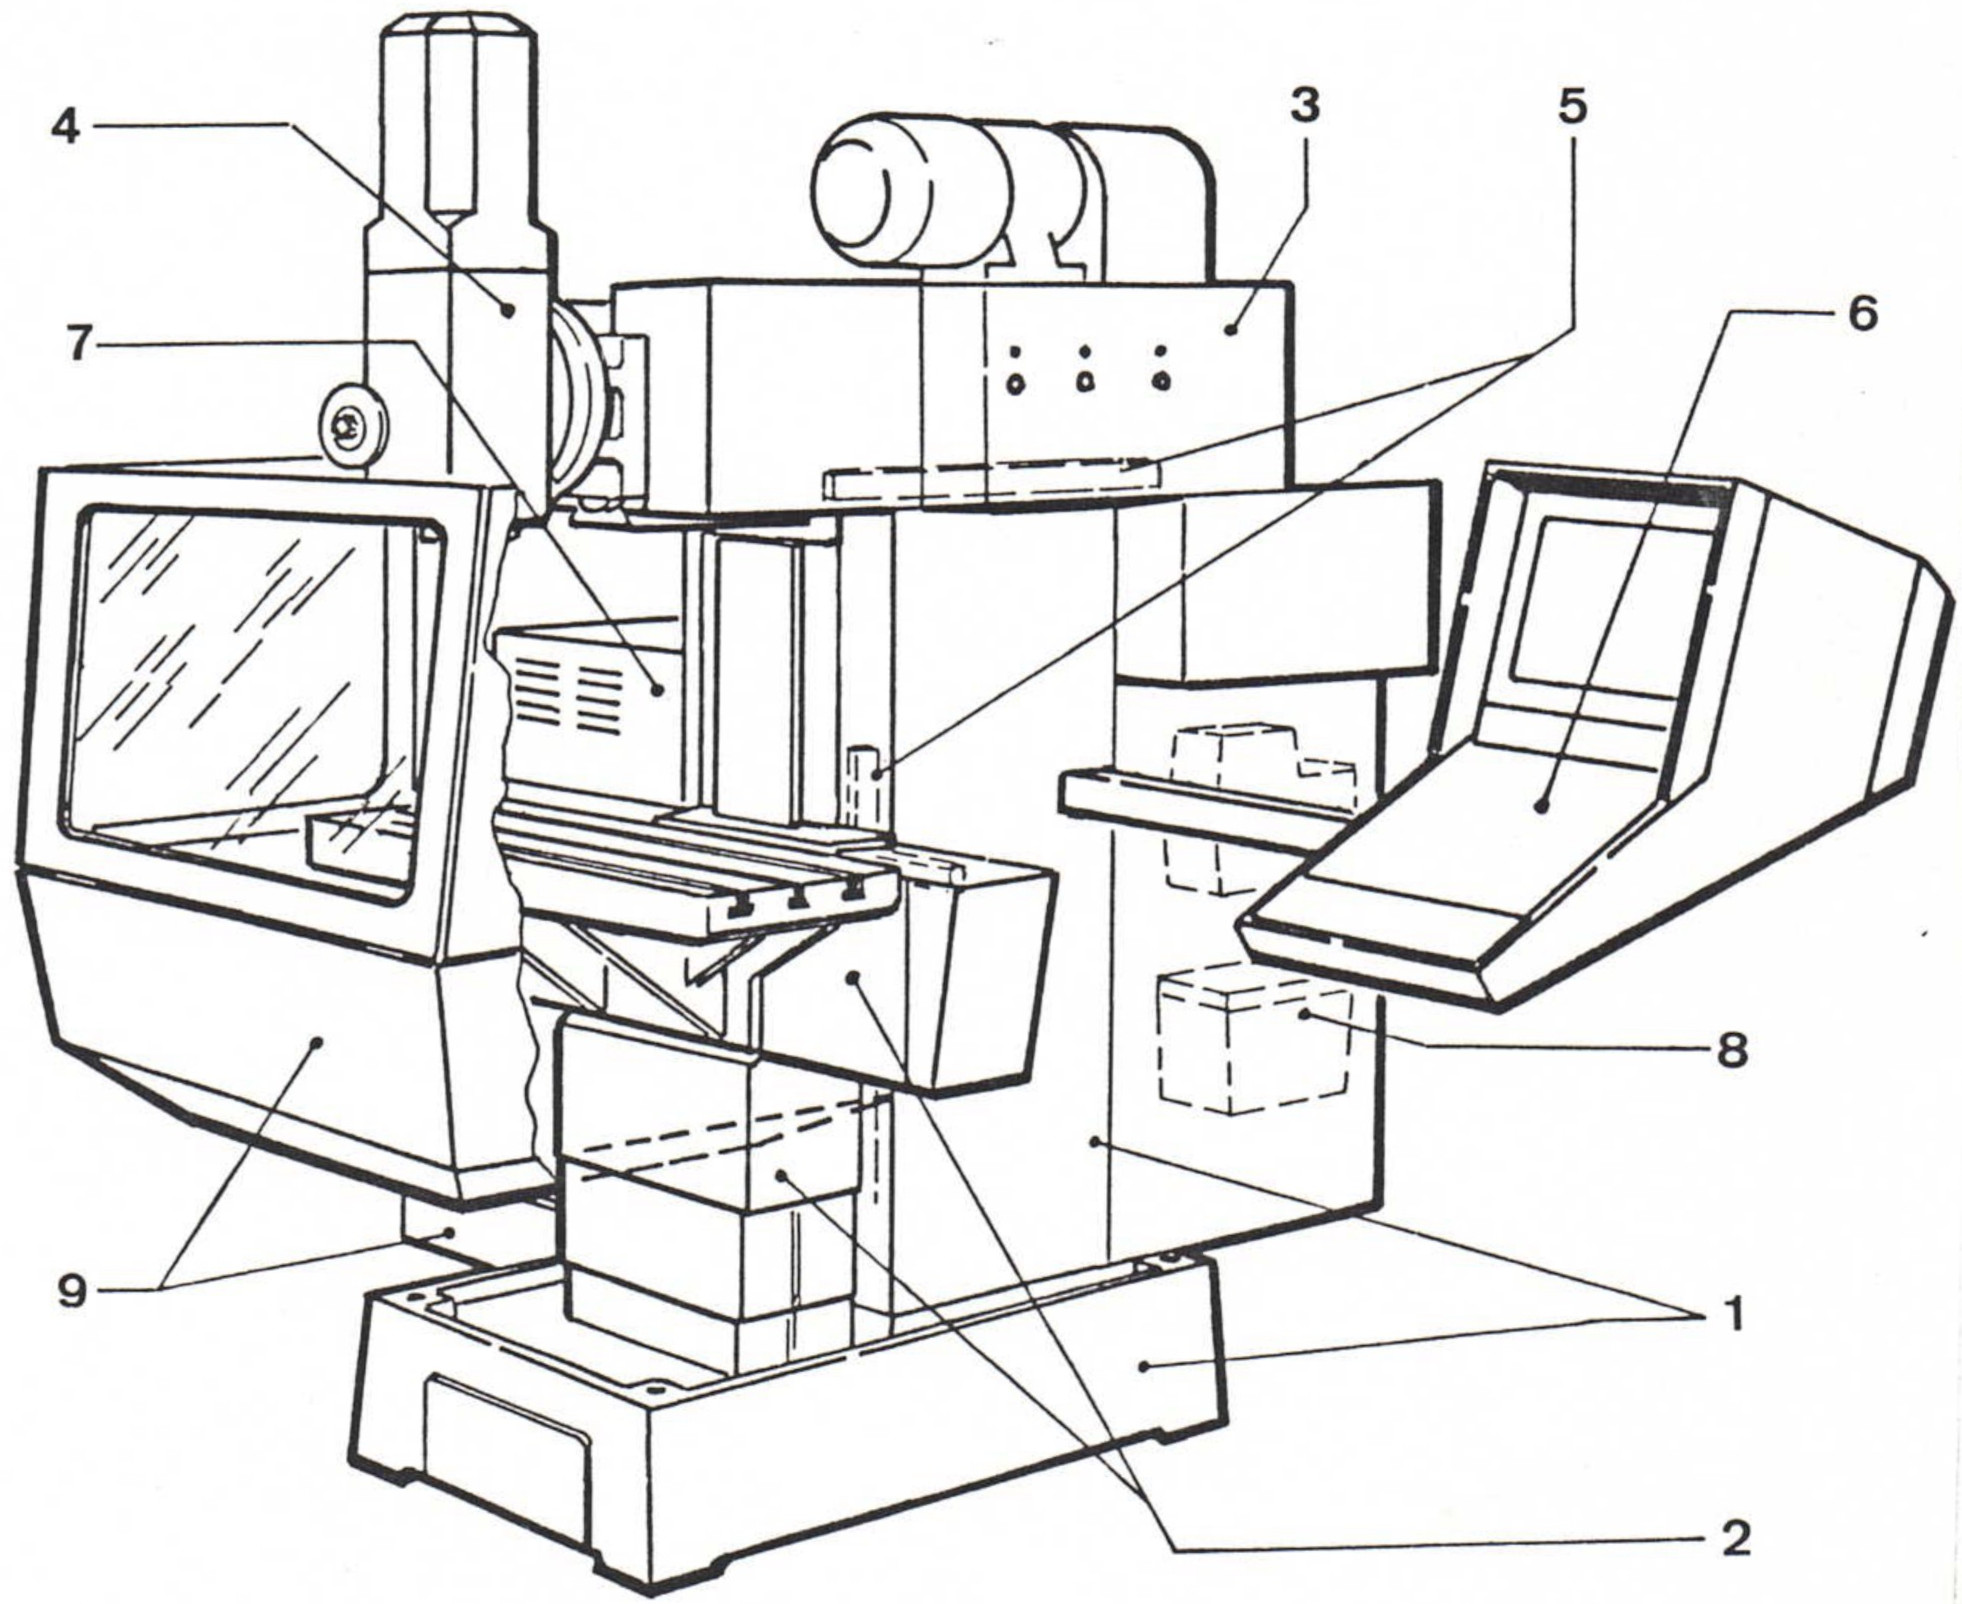
\includegraphics[width=0.8\textwidth]{chapter2/machine_overview.jpg}
    \caption{}
    \label{fig:machine_overview}
\end{figure}

\vspace{3cm}

\begin{enumerate}[itemsep=1pt,parsep=0pt]
    \item Machine stand with base and Y-axis feed drive
    \item Cross support with vertical mounting table and X-axis feed drive
    \item Spindle head with horizontal working spindle and Z-axis feed drive
    \item Vertical milling head with vertical working spindle
    \item Measuring systems
    \item CNC control
    \item Electrical system
    \item Central lubrication system / hydraulic system
    \item Coolant system / splash guard
\end{enumerate}

\notebox{NOTE}{Description of the operating elements for the worktables can be found in Section 4 of the operator's manual.}

\sectionLikeSubsection{Description of Machine Components}

\subsection{Machine Stand with Base}

\begin{figure}[h]
    \centering
    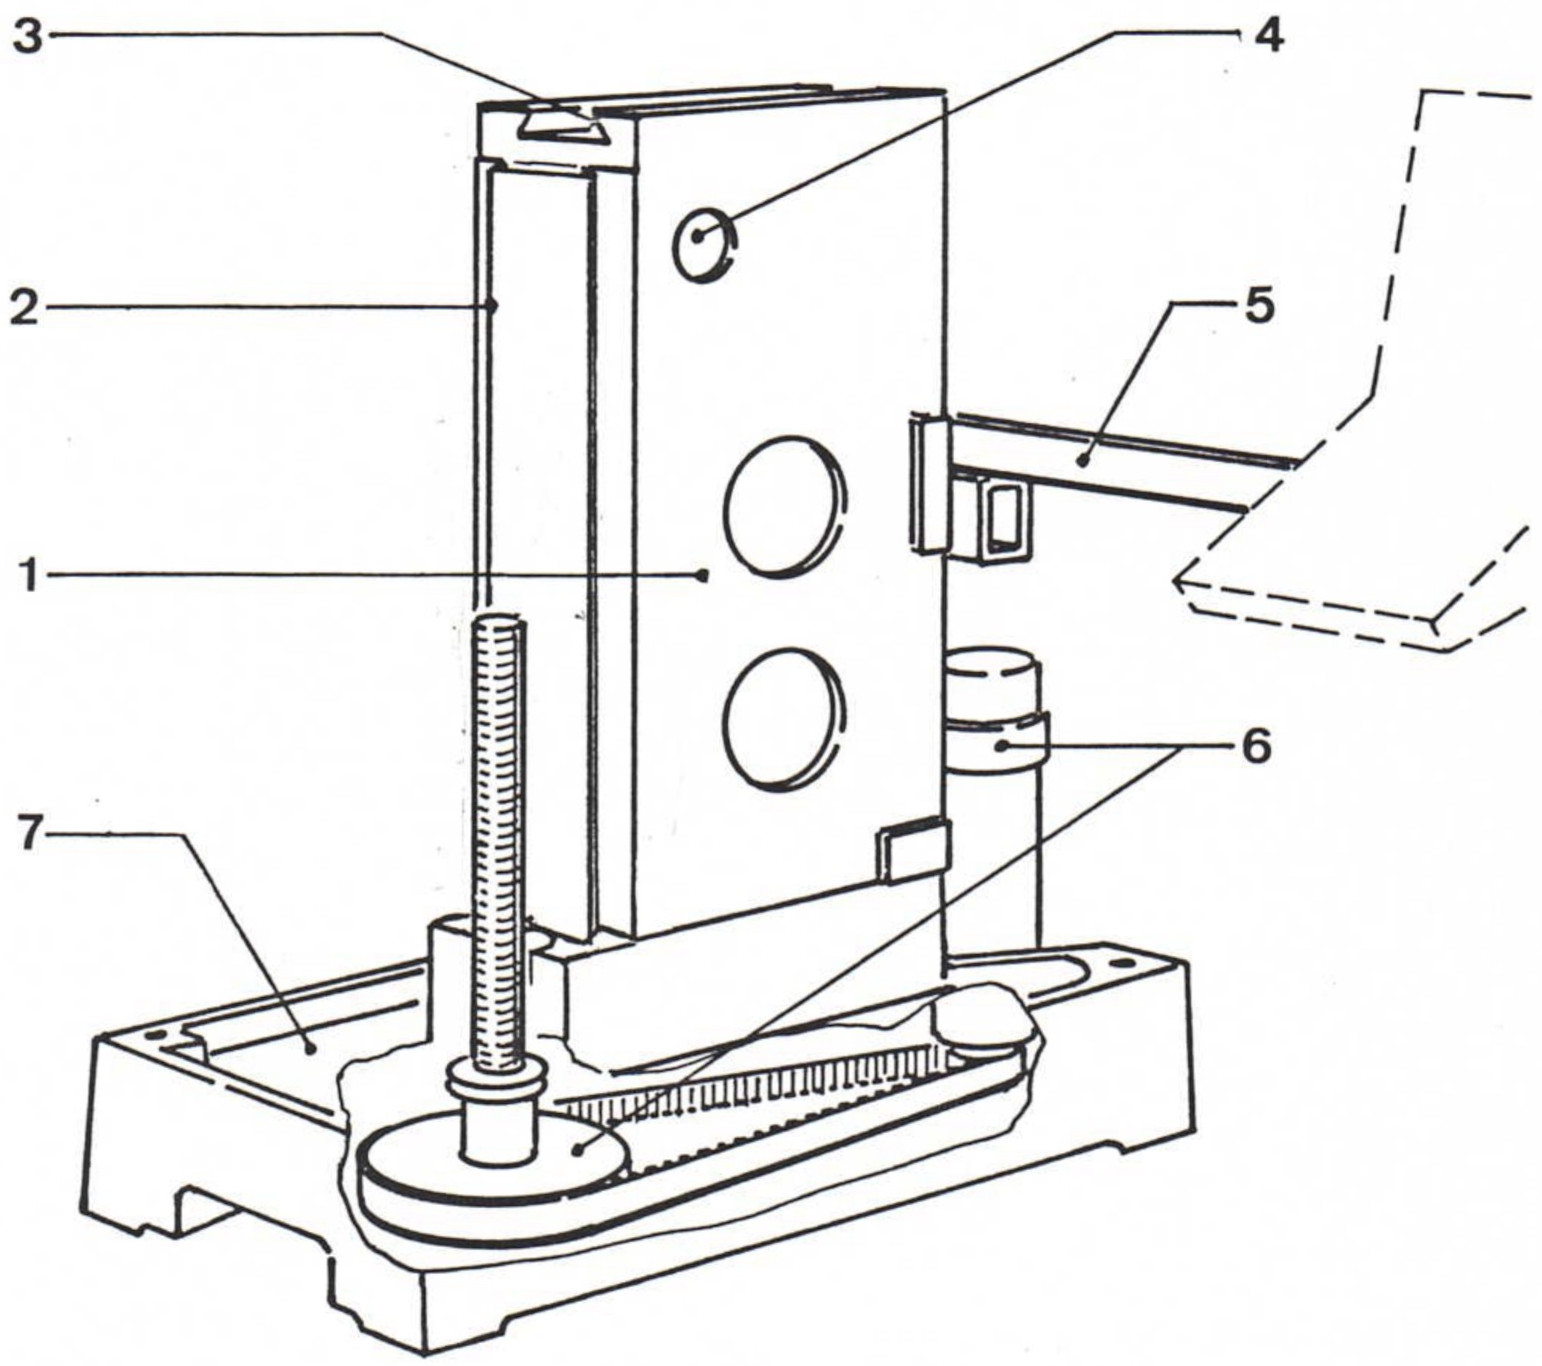
\includegraphics[width=0.6\textwidth]{chapter2/machine_stand.jpg}
    \caption{Diagram of the machine stand and its components.}
    \label{fig:machine_stand}
\end{figure}

\noindent The numbered components in the diagram are:
\begin{enumerate}[itemsep=1pt,parsep=0pt]
    \item Machine stand
    \item Dovetail guide for cross support
    \item Spindle head guide
    \item Opening for transporting the machine
    \item Swivel arm for control panel
    \item Y-axis feed drive
    \item Stand base
\end{enumerate}

\noindent The machine stand (1) with stand base (7) serves as the structural support for the other assemblies.

\vspace{.3cm}

\noindent The dovetail guide (2) on the front allows the vertical slide of the cross support to move smoothly.

\vspace{.3cm}

\noindent The mating surfaces of the spindle head (3) on the upper section of the \\machine stand are coated with the same plastic sliding material as the mating surface of the cross support.

\vspace{.3cm}

\noindent In the upper half of the stand, there is a continuous opening (4) designed to accommodate the transport rod.

\vspace{.3cm}

\noindent The Y-axis feed drive (6) is housed within the stand base (7).

\vfill
\clearpage

\subsection{Cross Support}

\begin{minipage}{0.5\textwidth}
    \begin{enumerate}[itemsep=1pt,parsep=0pt]
        \item Longitudinal slide
        \item Vertical slide, Y-axis
        \item DC motor, Y-axis
        \item Timing belt, Y-axis
        \item Ball screw, Y-axis
        \item Dovetail guide, Y-axis
        \item Ball screw, X-axis
        \item Timing belt, X-axis
        \item DC motor, X-axis
        \item Dovetail flat guide, X-axis
    \end{enumerate}
\end{minipage}%
\begin{minipage}{0.5\textwidth}
    \centering
    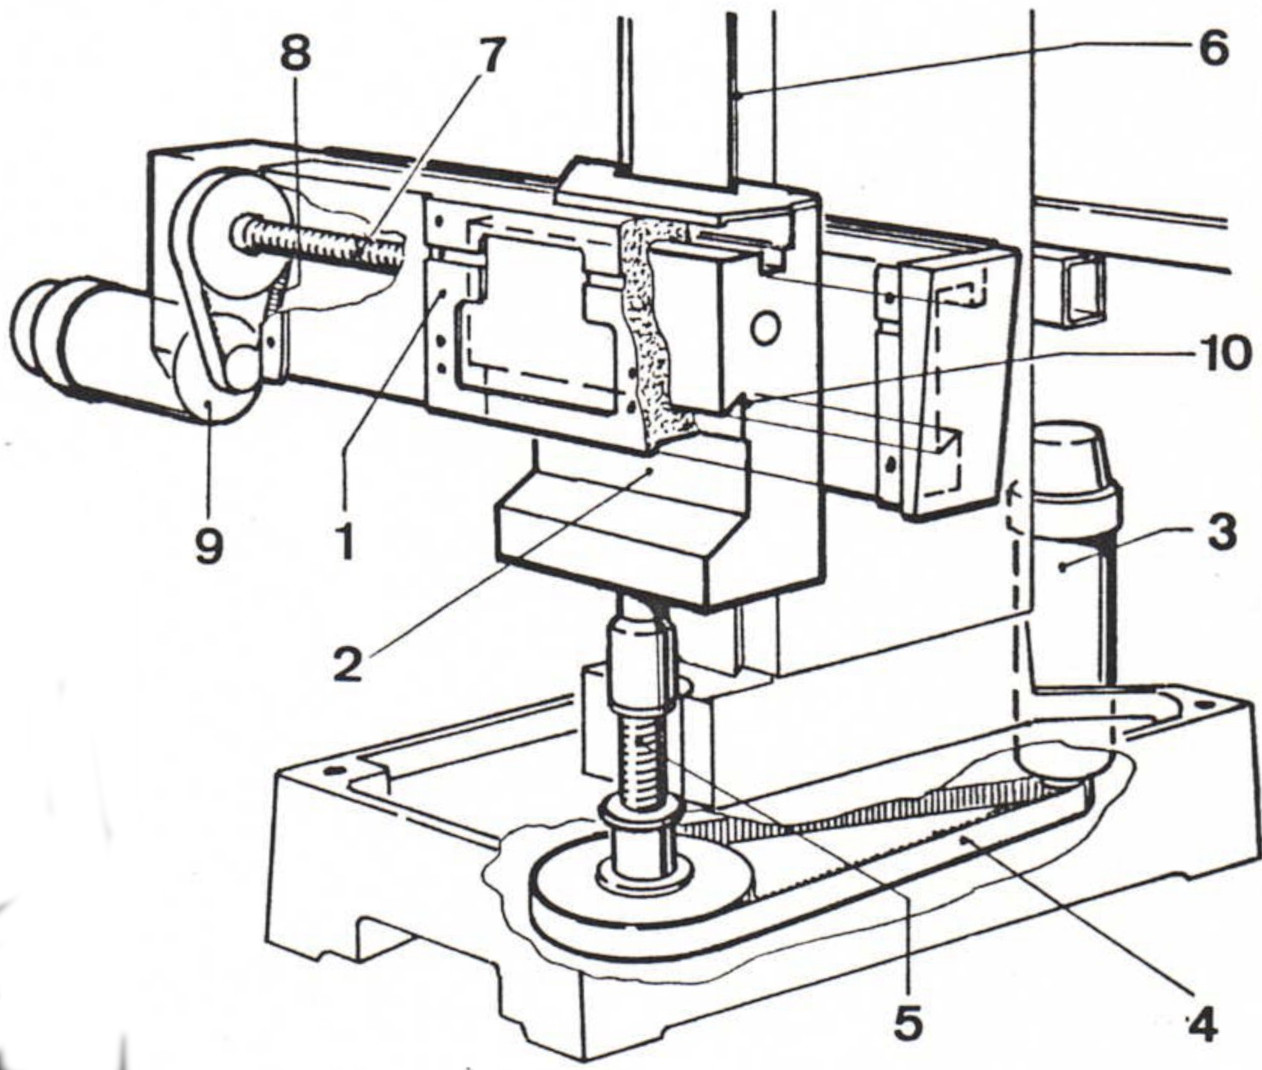
\includegraphics[width=0.9\textwidth]{chapter2/cross_support.jpg}
    \captionof{figure}{}
    \label{fig:cross_support}
\end{minipage}

\vspace{1cm}

\noindent The cross support carries out the necessary longitudinal and vertical\\ movements for workpiece machining.

\vspace{.3cm}

\noindent It consists of the longitudinal slide "vertical mounting table" (X-axis) (1) and the vertical slide (Y-axis) (2).

\vspace{.3cm}

\noindent The worktables are mounted on the vertical mounting table; see Chapter 4.

\vspace{.3cm}

\noindent A DC motor (3), along with timing belts (4) and a ball screw (5), provides the feed drive for the Y-axis.

\vspace{.3cm}

\noindent The vertical slide moves along the dovetail guide (10) on the machine stand. The mating surfaces on the support are coated with a plastic sliding material that has excellent wear resistance, emergency running properties, damping characteristics, and friction performance, allowing smooth sliding \\(eliminating the stick-slip effect).

\vspace{.3cm}

\noindent The longitudinal slide is guided by the vertical slide using a dovetail guide (6). Its mating surfaces are also coated with the specialized sliding \\material.

\vspace{.3cm}

\noindent All guides are equipped with wipers to protect against chips, dirt, and \\coolant contamination and are automatically lubricated via a central \\lubrication system.

\vspace{.3cm}

\noindent The longitudinal slide (X-axis) is driven by a DC motor (9) through a timing belt (8) and a ball screw (7).

\vfill
\clearpage

\subsection{Spindle Head}

\begin{minipage}{0.5\textwidth}
    \begin{enumerate}[itemsep=1pt,parsep=0pt]
        \item Spindle head housing
        \item Main motor
        \item Gearbox
        \item Poly V-belt
        \item Timing belt
        \item DC motor, Z-axis
        \item Ball screw
        \item Horizontal working spindle
        \item Vertical milling head drive shaft
    \end{enumerate}
\end{minipage}%
\begin{minipage}{0.5\textwidth}
    \centering
    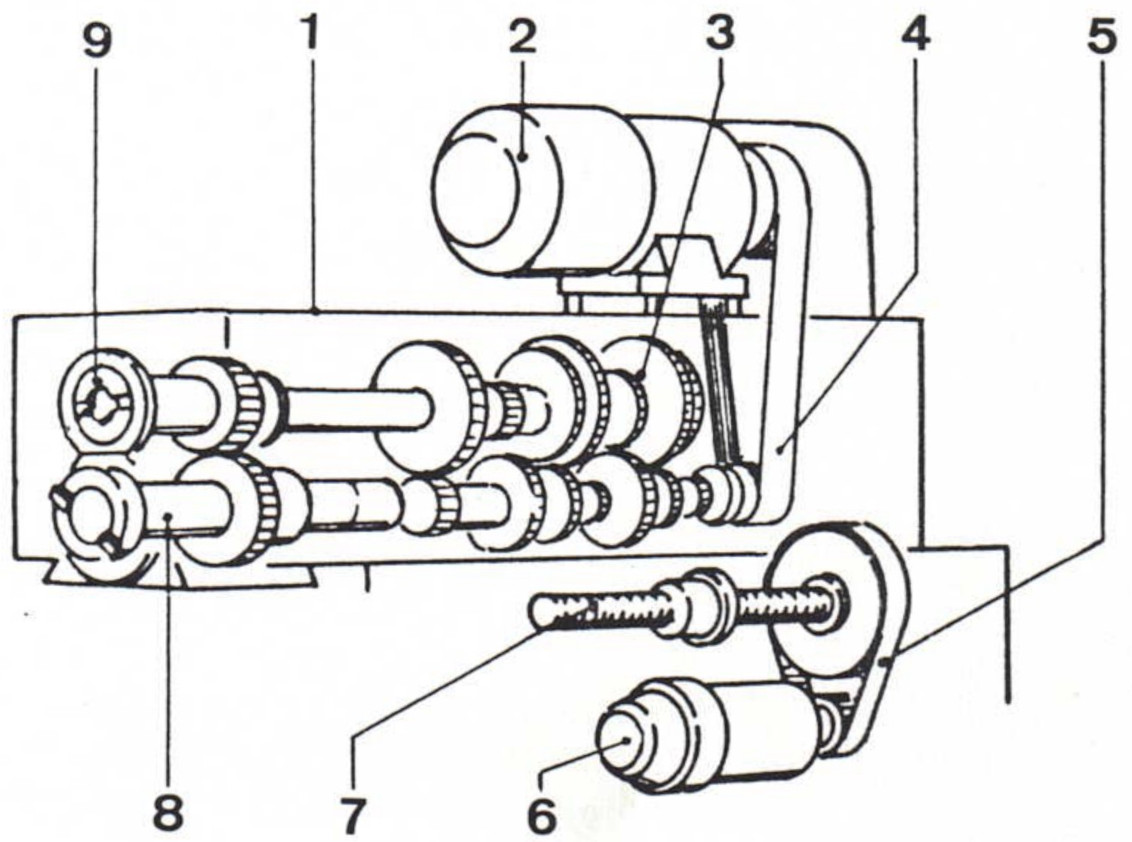
\includegraphics[width=0.9\textwidth]{chapter2/spindle_head.jpg}
    \captionof{figure}{}
    \label{fig:spindle_head}
\end{minipage}

\vspace{1cm}

\noindent The spindle head (1) is equipped with a dovetail guide and is mounted on the upper side of the machine stand.

\vspace{.3cm}

\noindent Its front side accommodates either the vertical milling head or the \\counterholder for horizontal milling (see also pages 3.05-1, 3.07-1 to \\3.09-1).

\vspace{.3cm}

\noindent The dovetail guide is fitted with wipers to prevent the ingress of chips, dirt, and coolant.

\vspace{.3cm}

\noindent The mating surfaces on the machine stand are coated with the same specialized sliding material as those on the cross support.

\vspace{.3cm}

\noindent The three-phase main motor (2) is mounted on top of the spindle head.

\vspace{.3cm}

\noindent The main motor's torque is transmitted via a poly V-belt (4) and an integrated 18-speed gearbox (3) within the spindle head to the working spindle (8).

\vspace{.3cm}

\noindent The working spindle (8) runs in five preloaded precision spindle bearings, which are permanently lubricated for maintenance-free operation.

\vspace{.3cm}

\noindent A DC motor (6) mounted beneath the spindle head, together with the timing belt (5) and ball screw (7), drives the Z-axis feed motion.

\vfill
\clearpage

\subsection{Vertical Milling Head}

\begin{minipage}{0.5\textwidth}
    \begin{enumerate}[itemsep=1pt,parsep=0pt]
        \item Spindle head
        \item Milling head extension arm
        \item Intermediate flange
        \item Milling head housing
        \item Vertical working spindle
        \item Quill adjustment mechanism
    \end{enumerate}
\end{minipage}%
\begin{minipage}{0.5\textwidth}
    \centering
    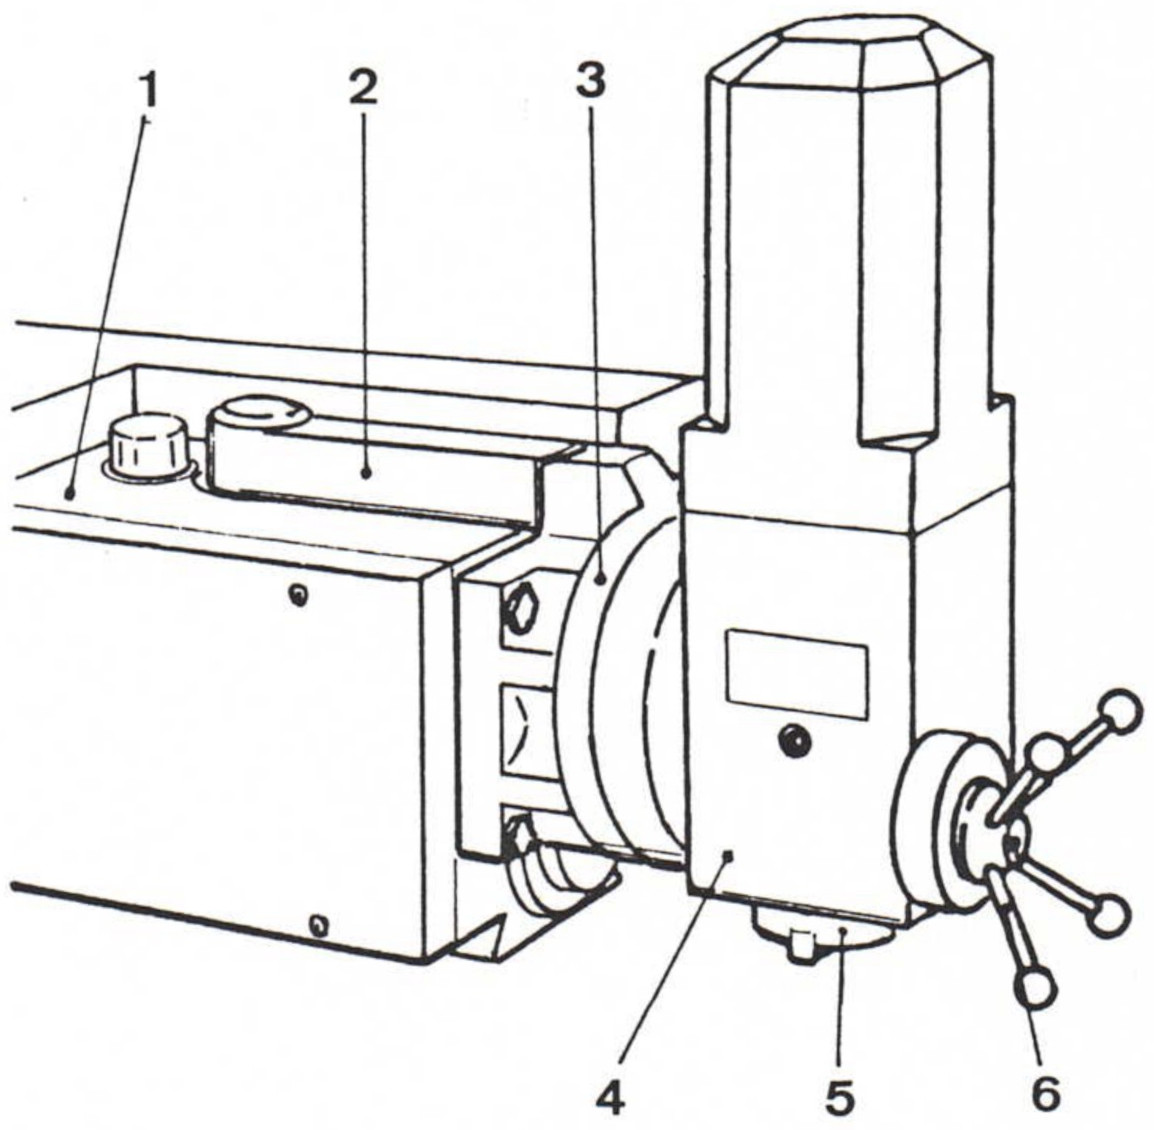
\includegraphics[width=0.9\textwidth]{chapter2/vertical_milling_head.jpg}
    \captionof{figure}{}
    \label{fig:vertical_milling_head}
\end{minipage}

\vspace{1cm}

\noindent The vertical milling head is mounted on top of the spindle head (1) with a pivotable extension arm. This allows it to be swung out of the working area when not in use.

\vspace{.3cm}

\noindent The milling head housing (4) is mounted on the intermediate flange (3) and can be swiveled 90° in both directions.

\vspace{.3cm}

\noindent The vertical working spindle (5) is supported by four preloaded precision spindle bearings within a quill. Due to its lifetime lubrication, these bearings are maintenance-free.

\vspace{.3cm}

\noindent The quill can be extended using the quill adjustment mechanism (6).

\vspace{.3cm}

\noindent Detailed instructions on operation and handling can be found on pages 3.07-1 to 3.09-1.

\newpage
\subsection{Measuring Systems}

The measuring systems operate contact-free and maintenance-free, with a \\resolution of 0.001 mm. Protective covers shield them from the ingress of chips and coolant.

\vspace{0.3cm}

\noindent A detailed functional description of the measuring systems can be found in Chapter 5.

\vspace{0.3cm}

\noindent The X-axis measuring system is installed at the top of the cross support.

\vspace{0.3cm}

\noindent The Y-axis measuring system is located on the left side of the machine stand.

\vspace{0.3cm}

\noindent The Z-axis measuring system is mounted on the left side of the spindle head.

\vspace{0.3cm}

\noindent Thermal expansion of the spindle head, caused by the working spindle heating up, is compensated by the Z-axis measuring system.

\vspace{0.3cm}

\noindent To ensure high measurement accuracy, an invar rod (2) fixed to the spindle head compensates for thermal expansion by adjusting the scale bar (4), \\maintaining precise measurements throughout the machine's operational life.

\vspace{0.5cm}

\noindent\textbf{\uline{Z-Axis Measuring System}}

\begin{figure}[h]
    \centering
    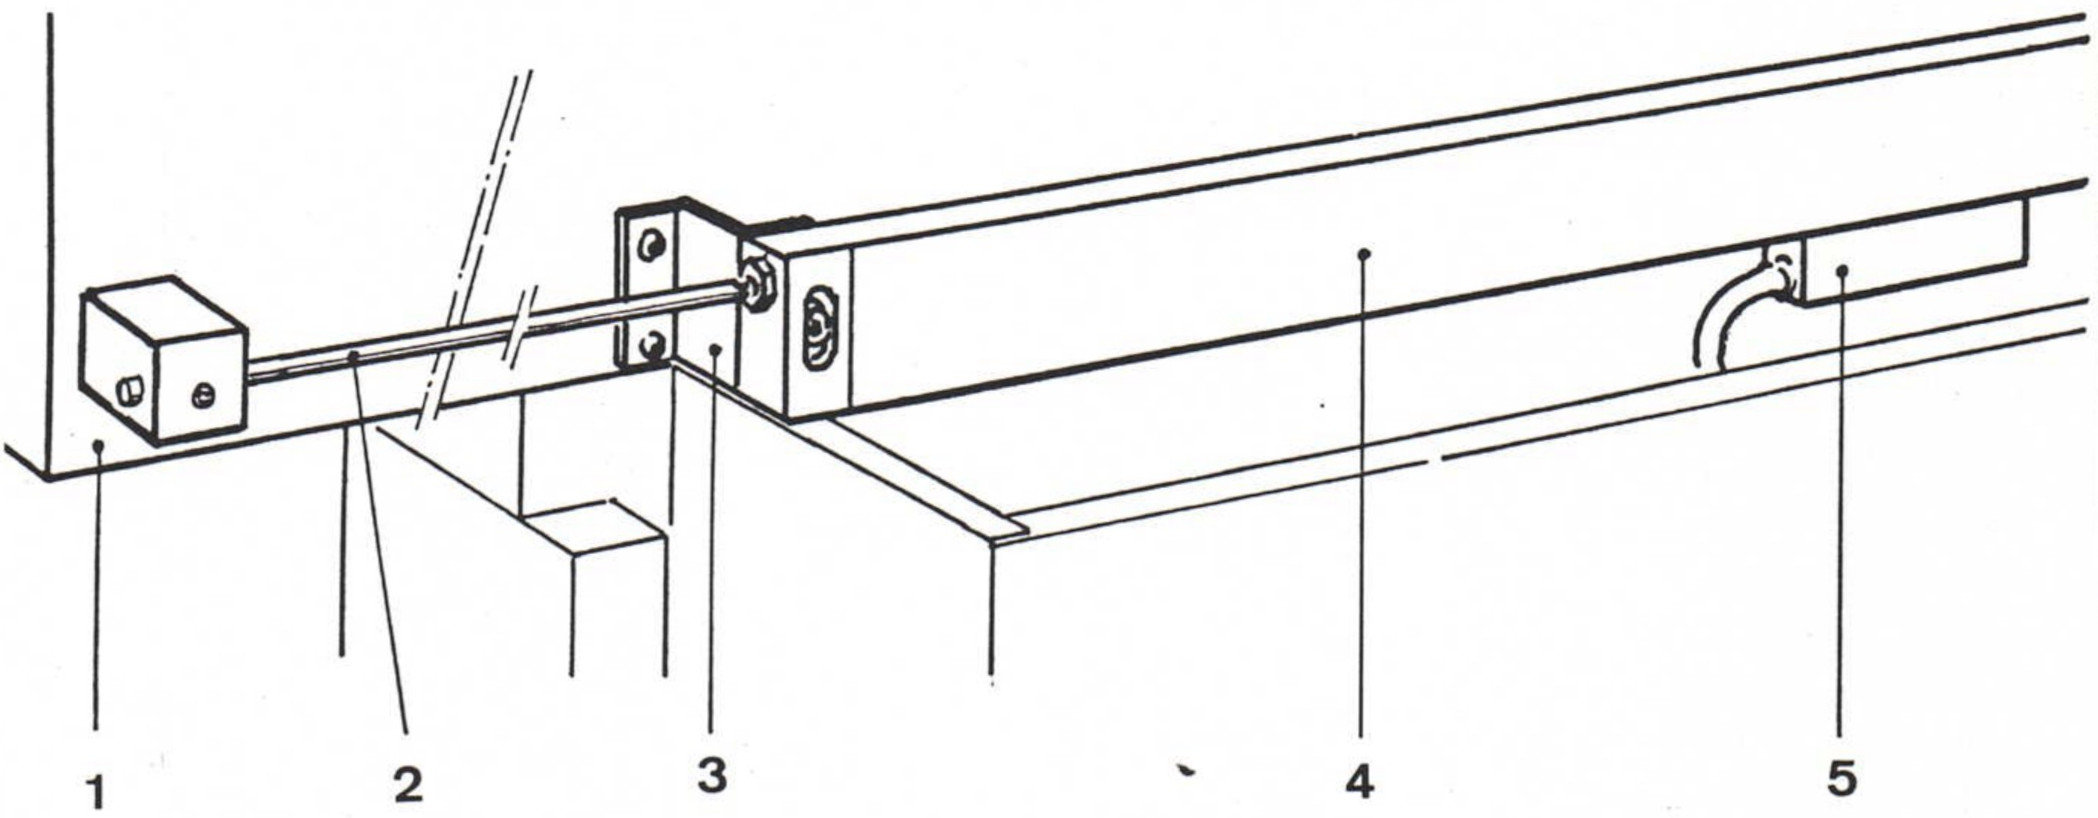
\includegraphics[width=0.9\textwidth]{chapter2/measuring_system_z_axis.jpg}
    \caption{}
    \label{fig:measuring_system_z}
\end{figure}

\begin{enumerate}[itemsep=1pt,parsep=0pt]
    \item Spindle head
    \item Invar rod
    \item Suspension strips
    \item Scale bar, Z-axis
    \item Measuring head
\end{enumerate}

\newpage

\subsection{CNC Control 432 E/Graphics}

The CNC control unit is housed in the control cabinet (5), while the control panel (2) and screen (3) are mounted in a control console. This console (4) is rotatable and is attached to a swivel arm (1) on the left side of the machine.

\vspace{0.3cm}

\noindent The construction, function, and programming of the control system are \\described in the CNC 432/10-Graphics manual.

\vspace{-.3cm}


\begin{minipage}[b]{0.5\textwidth}
    \textbf{\uline{CNC Control 432 E/Graphics}}
    \begin{enumerate}[itemsep=1pt,parsep=0pt]
        \item Swivel arm
        \item Control panel
        \item Screen
        \item Control console
    \end{enumerate}
\end{minipage}%
\begin{minipage}{0.5\textwidth}
    \centering
    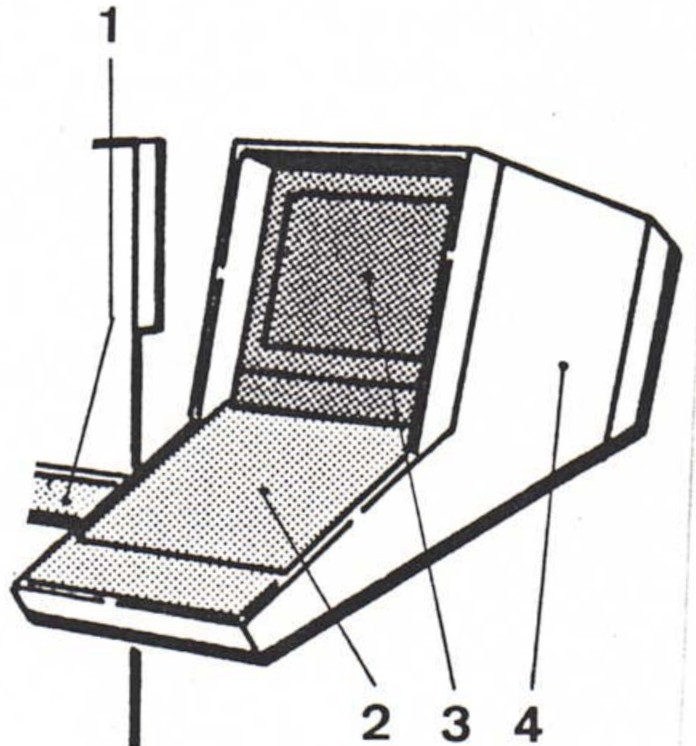
\includegraphics[width=0.6\textwidth]{chapter2/cnc_control.jpg}
    \captionof{figure}{}
    \label{fig:cnc_control}
\end{minipage}

\vspace{-1cm}

\subsection{Electrical System}

The control cabinet (5), located at the rear of the machine, contains the power module, which supplies energy to the machine’s drives.

\vspace{0.3cm}

\noindent It processes signals from the CNC 432 E control, regulates the drives, and protects against overcurrent.

\vspace{0.3cm}
\noindent Inside the control cabinet door (8) are the main switch (9) and the adjustment module (10).

\begin{minipage}[c]{0.45\textwidth}
    \begin{enumerate}[itemsep=1pt,parsep=0pt]
        \setcounter{enumi}{4}
        \item Control cabinet
        \item Transformer room
        \item Heat exchanger
        \item Control cabinet door
        \item Main switch
        \item Adjustment module
        \item CNC Control 432 E/Graphics
    \end{enumerate}

    \noindent The adjustment module contains the following switches:
\end{minipage}%
\begin{minipage}{0.6\textwidth}
    \centering
    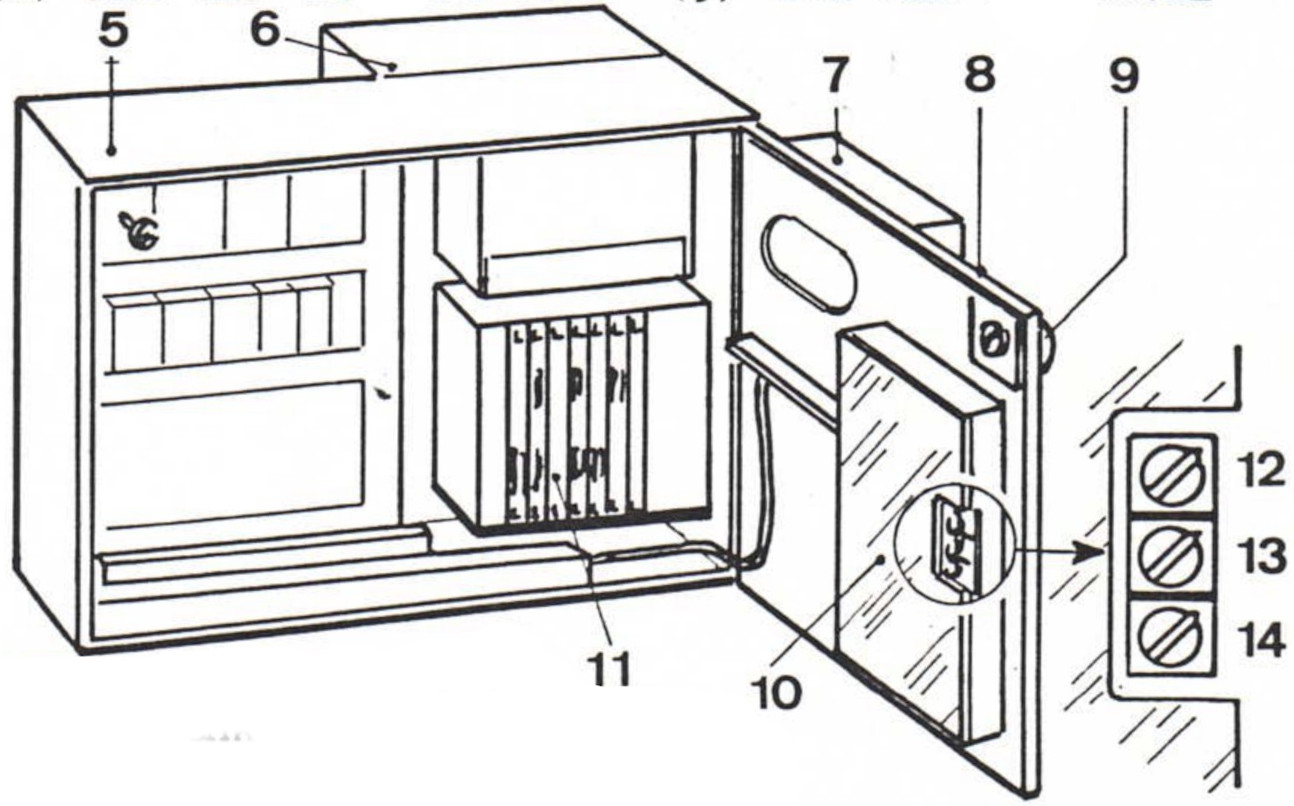
\includegraphics[width=\textwidth]{chapter2/electrical_system.jpg}
    % \captionof{figure}{}
    \label{fig:electrical_system}
\end{minipage}

\begin{textblock*}{\textwidth}(3cm, 21cm)  % Adjust coordinates as needed
    \begin{enumerate}[itemsep=1pt,parsep=0pt]
        \setcounter{enumi}{11}
        \item \textbf{Rotary switch (7S1):} "Brake Y-axis engaged/disengaged"
        \item \textbf{Rotary switch (19S1):} "Read machine constants"
        \item \textbf{Rotary switch (19S2):} "Test operation"
    \end{enumerate}
\end{textblock*}

\vspace{2cm}

\notebox{NOTE}{The numbers in parentheses correspond to circuit diagram labels.}

\section{Movement Directions}

\begin{figure}[h]
    \centering
    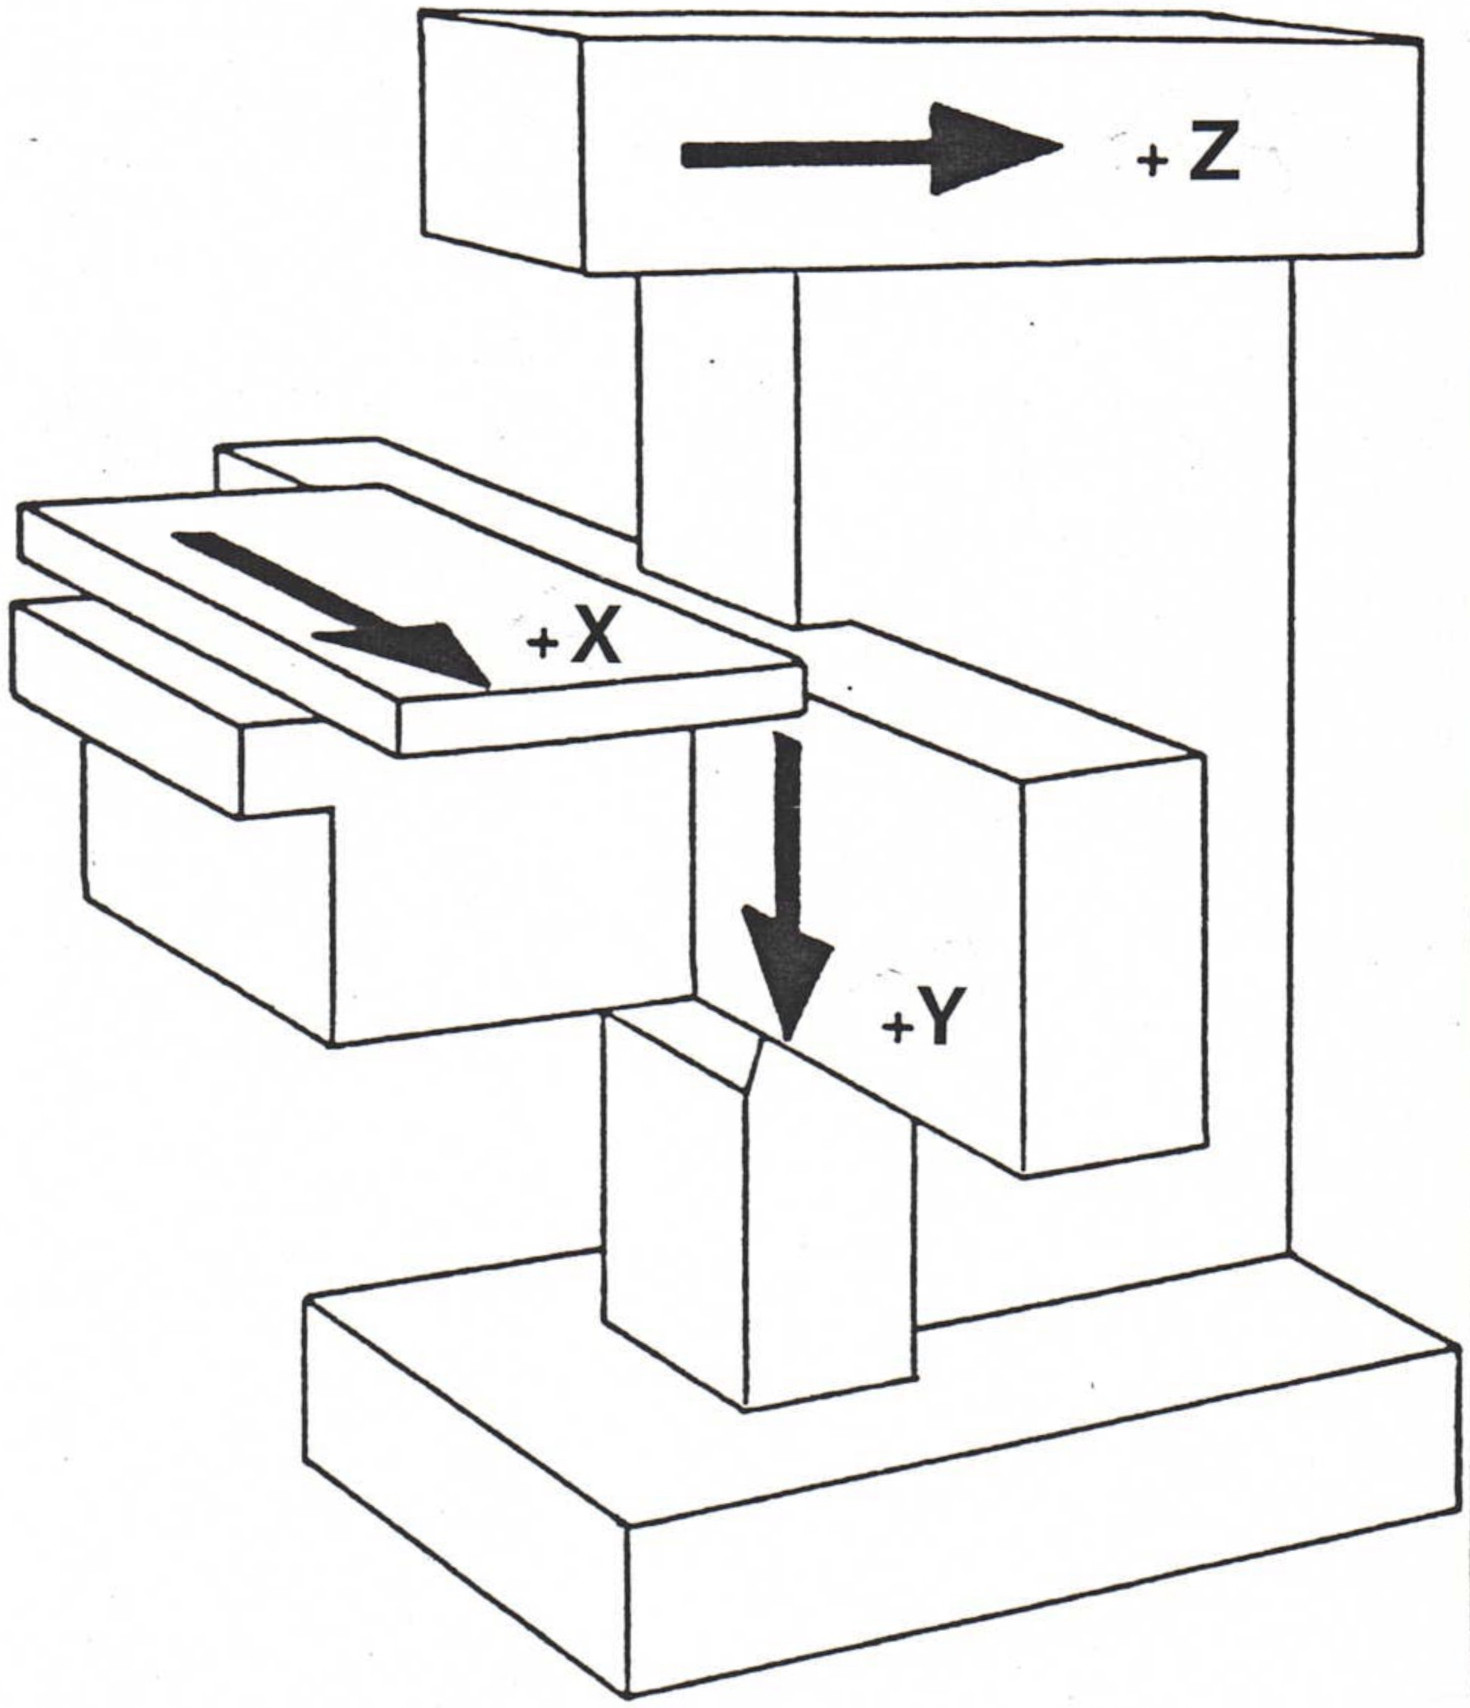
\includegraphics[width=0.8\textwidth]{chapter2/movement_directions.jpg}
\end{figure}

\vspace{0.5cm}

\noindent \textbf{Axis Definitions:}

\vspace{0.3cm}

\noindent \begin{tabular}{ l l }
\textbf{X-Axis} & Horizontal longitudinal movement of the vertical mounting table: \\
                & Left \enquote{-} or Right \enquote{+}. \\
\textbf{Y-Axis} & Vertical movement of the cross support: \\
                & Up \enquote{-} or Down \enquote{+}. \\
\textbf{Z-Axis} & Horizontal transverse movement of the spindle head: \\
                & Forward \enquote{-} or Backward \enquote{+}. \\
\end{tabular}

\section{Control Station (Machine)}

\begin{figure}[h]
    \centering
    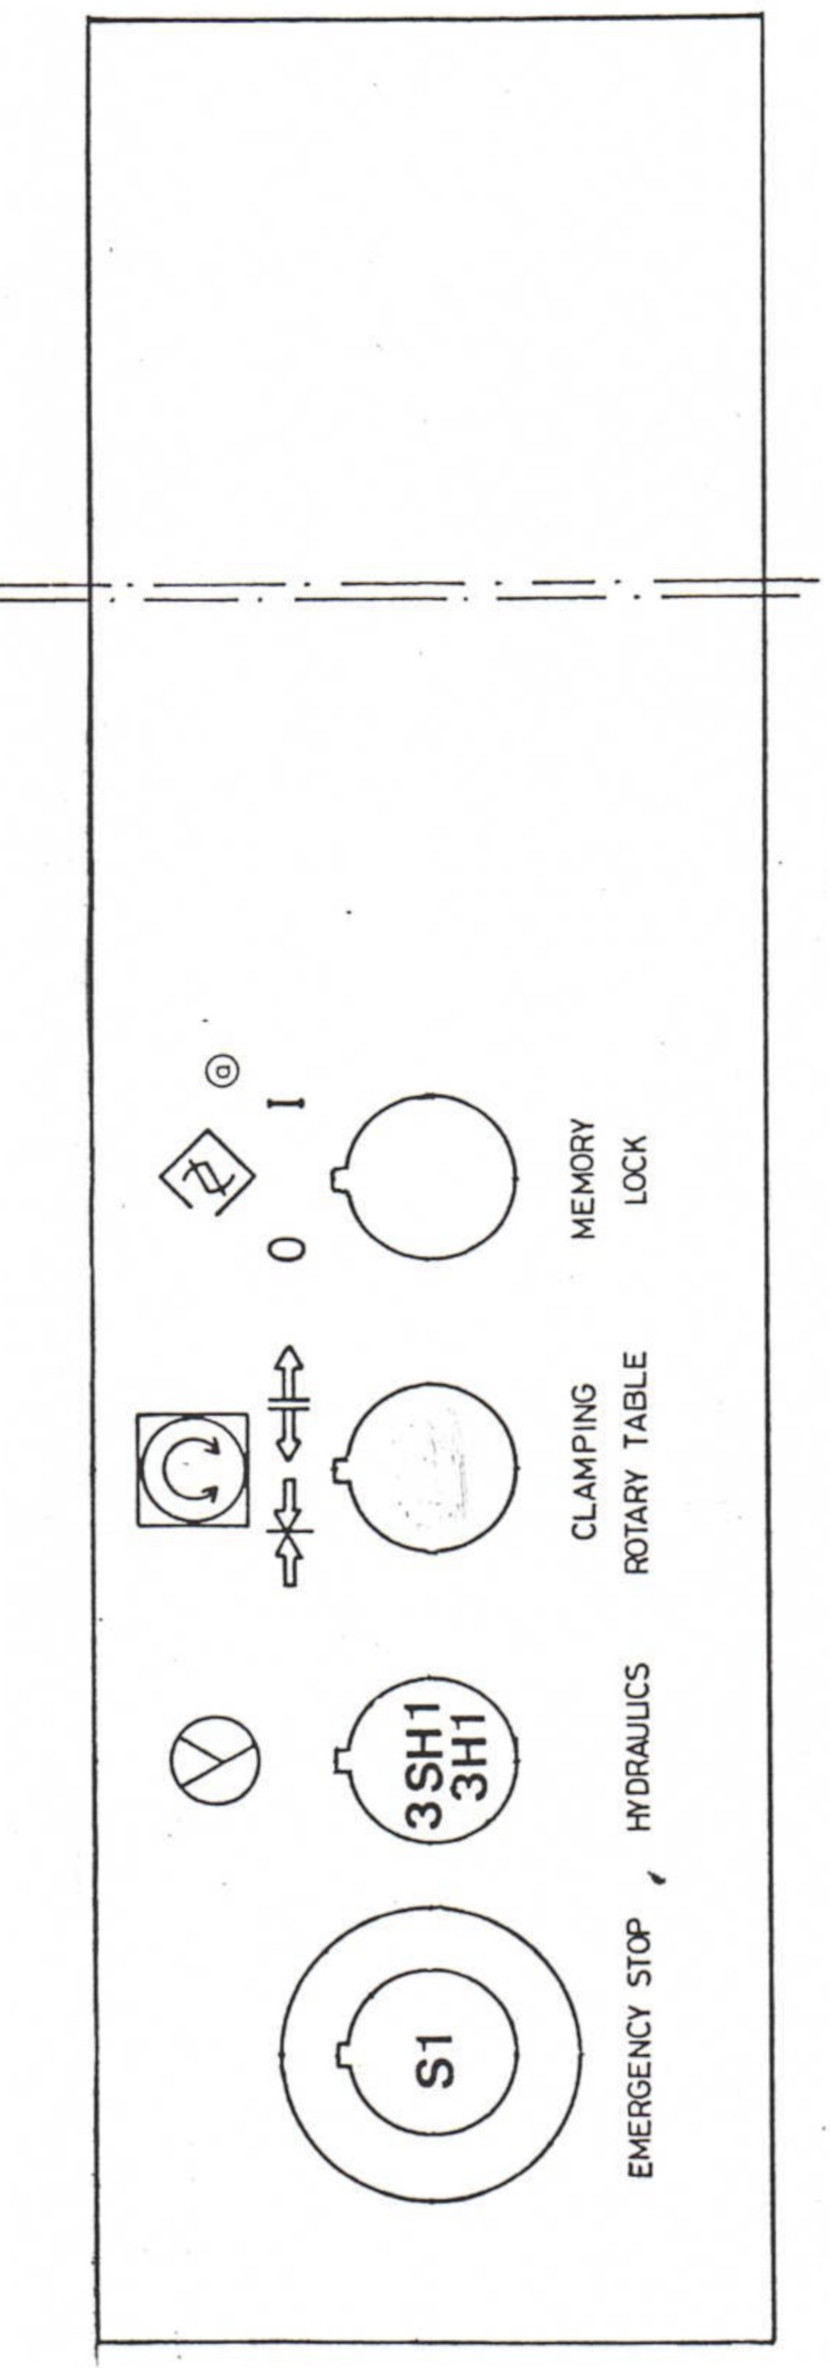
\includegraphics[width=0.38\textwidth]{chapter2/control_station.jpg} % Replace with actual filename
\end{figure}

\sectionLikeSubsection{Control Station - Function of the Operating Elements (Machine)}

\vspace{0.3cm}

\noindent % Remove paragraph indentation
\begin{tabular}{|c|l|p{10cm}|}
    \hline\hline
    \textbf{Nr.} & \textbf{Operating Element} & \textbf{Function} \\
    \hline\hline
    -S1-   & Emergency stop button & Emergency stop. All machine motors are immediately shut down.\footnotemark[11] \\
    \hline
    -3SH1- & Illuminated push button & Hydraulics, central lubrication, and control ON. \\
    -3H1-  & Indicator light & ON. \\
    \hline\hline
\end{tabular}

\vspace{0.5cm}

\footnotetext[11]{After activation, the red emergency stop button remains locked. Before restarting the machine, the locking mechanism must be released by turning the emergency stop button to the right.}

\setcounter{page}{4}

\sectionLikeSubsection{Handheld Control Unit}

\noindent
For ease of setup when machining a workpiece, the CNC 432 control system is also equipped with a handheld control unit. It enables the operation of the following functions:

\begin{itemize}[itemsep=1pt,parsep=0pt]
    \item Axis selection in positive or negative direction for each axis. Operating modes: SINGLE, AUTOMATIC, MANUAL
    \item Program creation via PLAY-BACK
    \item Machine status
    \item Feed rate control (potentiometer)
    \item Spindle feed HOLD
    \item Feed START
    \item Coolant ON/OFF
    \item Tool clamp RELEASE/CLAMP
    \item EMERGENCY STOP
\end{itemize}

\noindent
Safety activation is required for enabling the keyboard from the handheld control unit for safety reasons.

\vspace{0.3cm}

\notebox{NOTE}{For operation with the handheld control unit, see the separate CNC 432/Graphics operating manual.}

\vspace{0.3cm}

\notebox{WARNING}{On \enquote{E}-machines, the following keys are \uline{not activated}:}

\vspace{-0.6cm}

\begin{center}
    \fbox{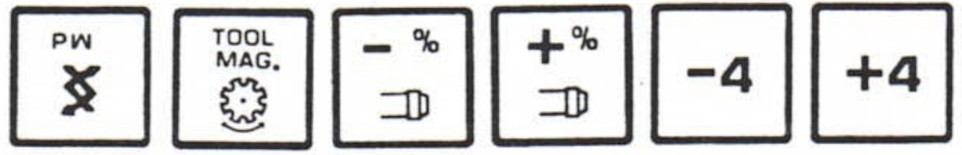
\includegraphics[width=0.4\textwidth]{chapter2/deactivated_keys.jpg}}
\end{center}

\vspace{-0.5cm}

\begin{figure}[h]
    \centering
    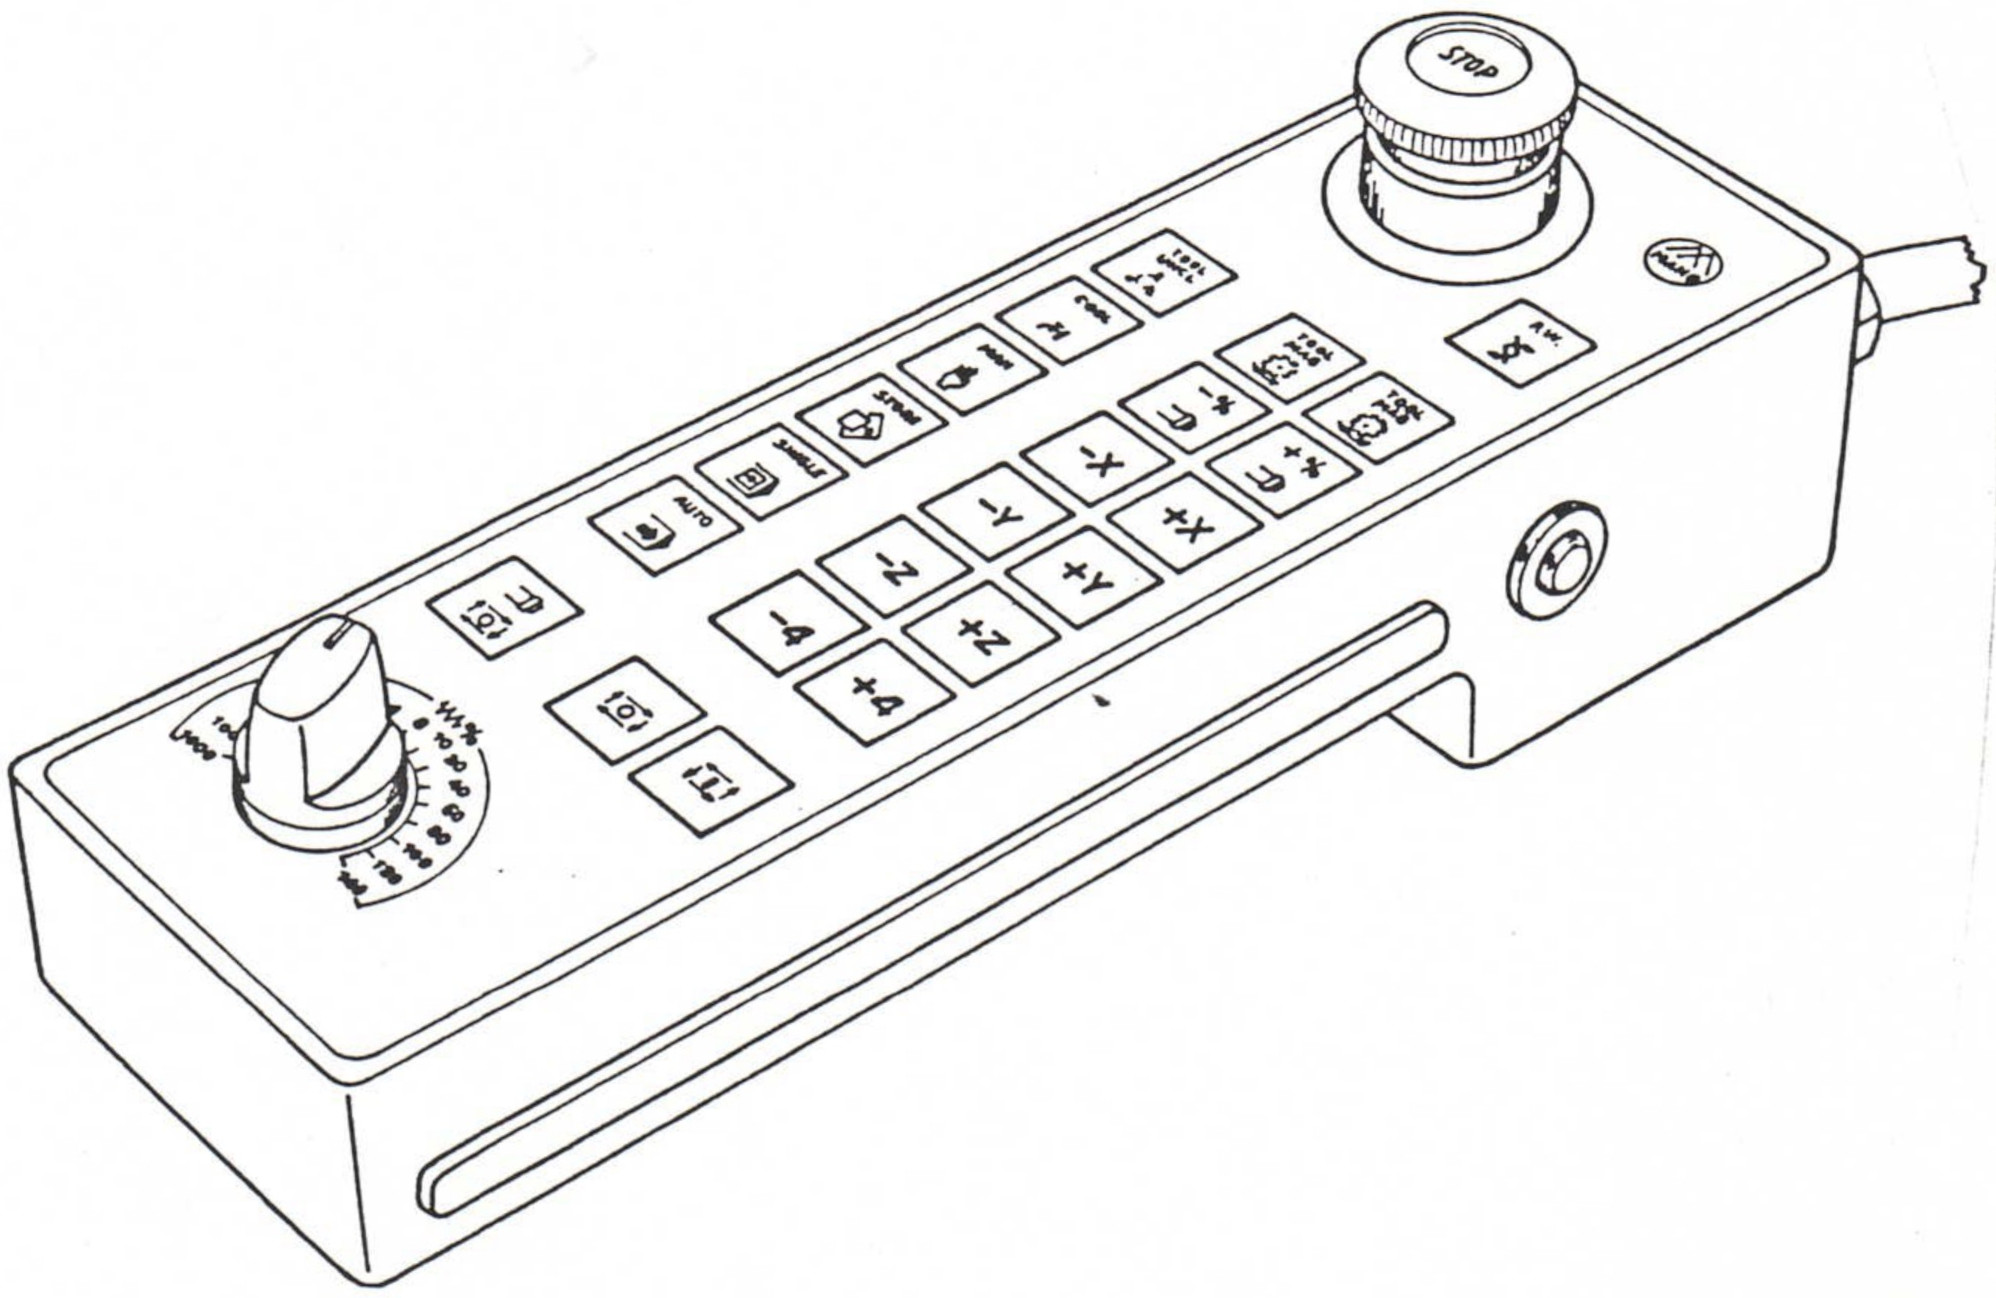
\includegraphics[width=0.9\textwidth]{chapter2/handheld_control.jpg}
\end{figure}

\section{Gear Train Schematic}
\setcounter{section}{10}
\begin{minipage}{\textwidth}
    \begin{adjustwidth}{-2cm}{-3cm}
        \centering
        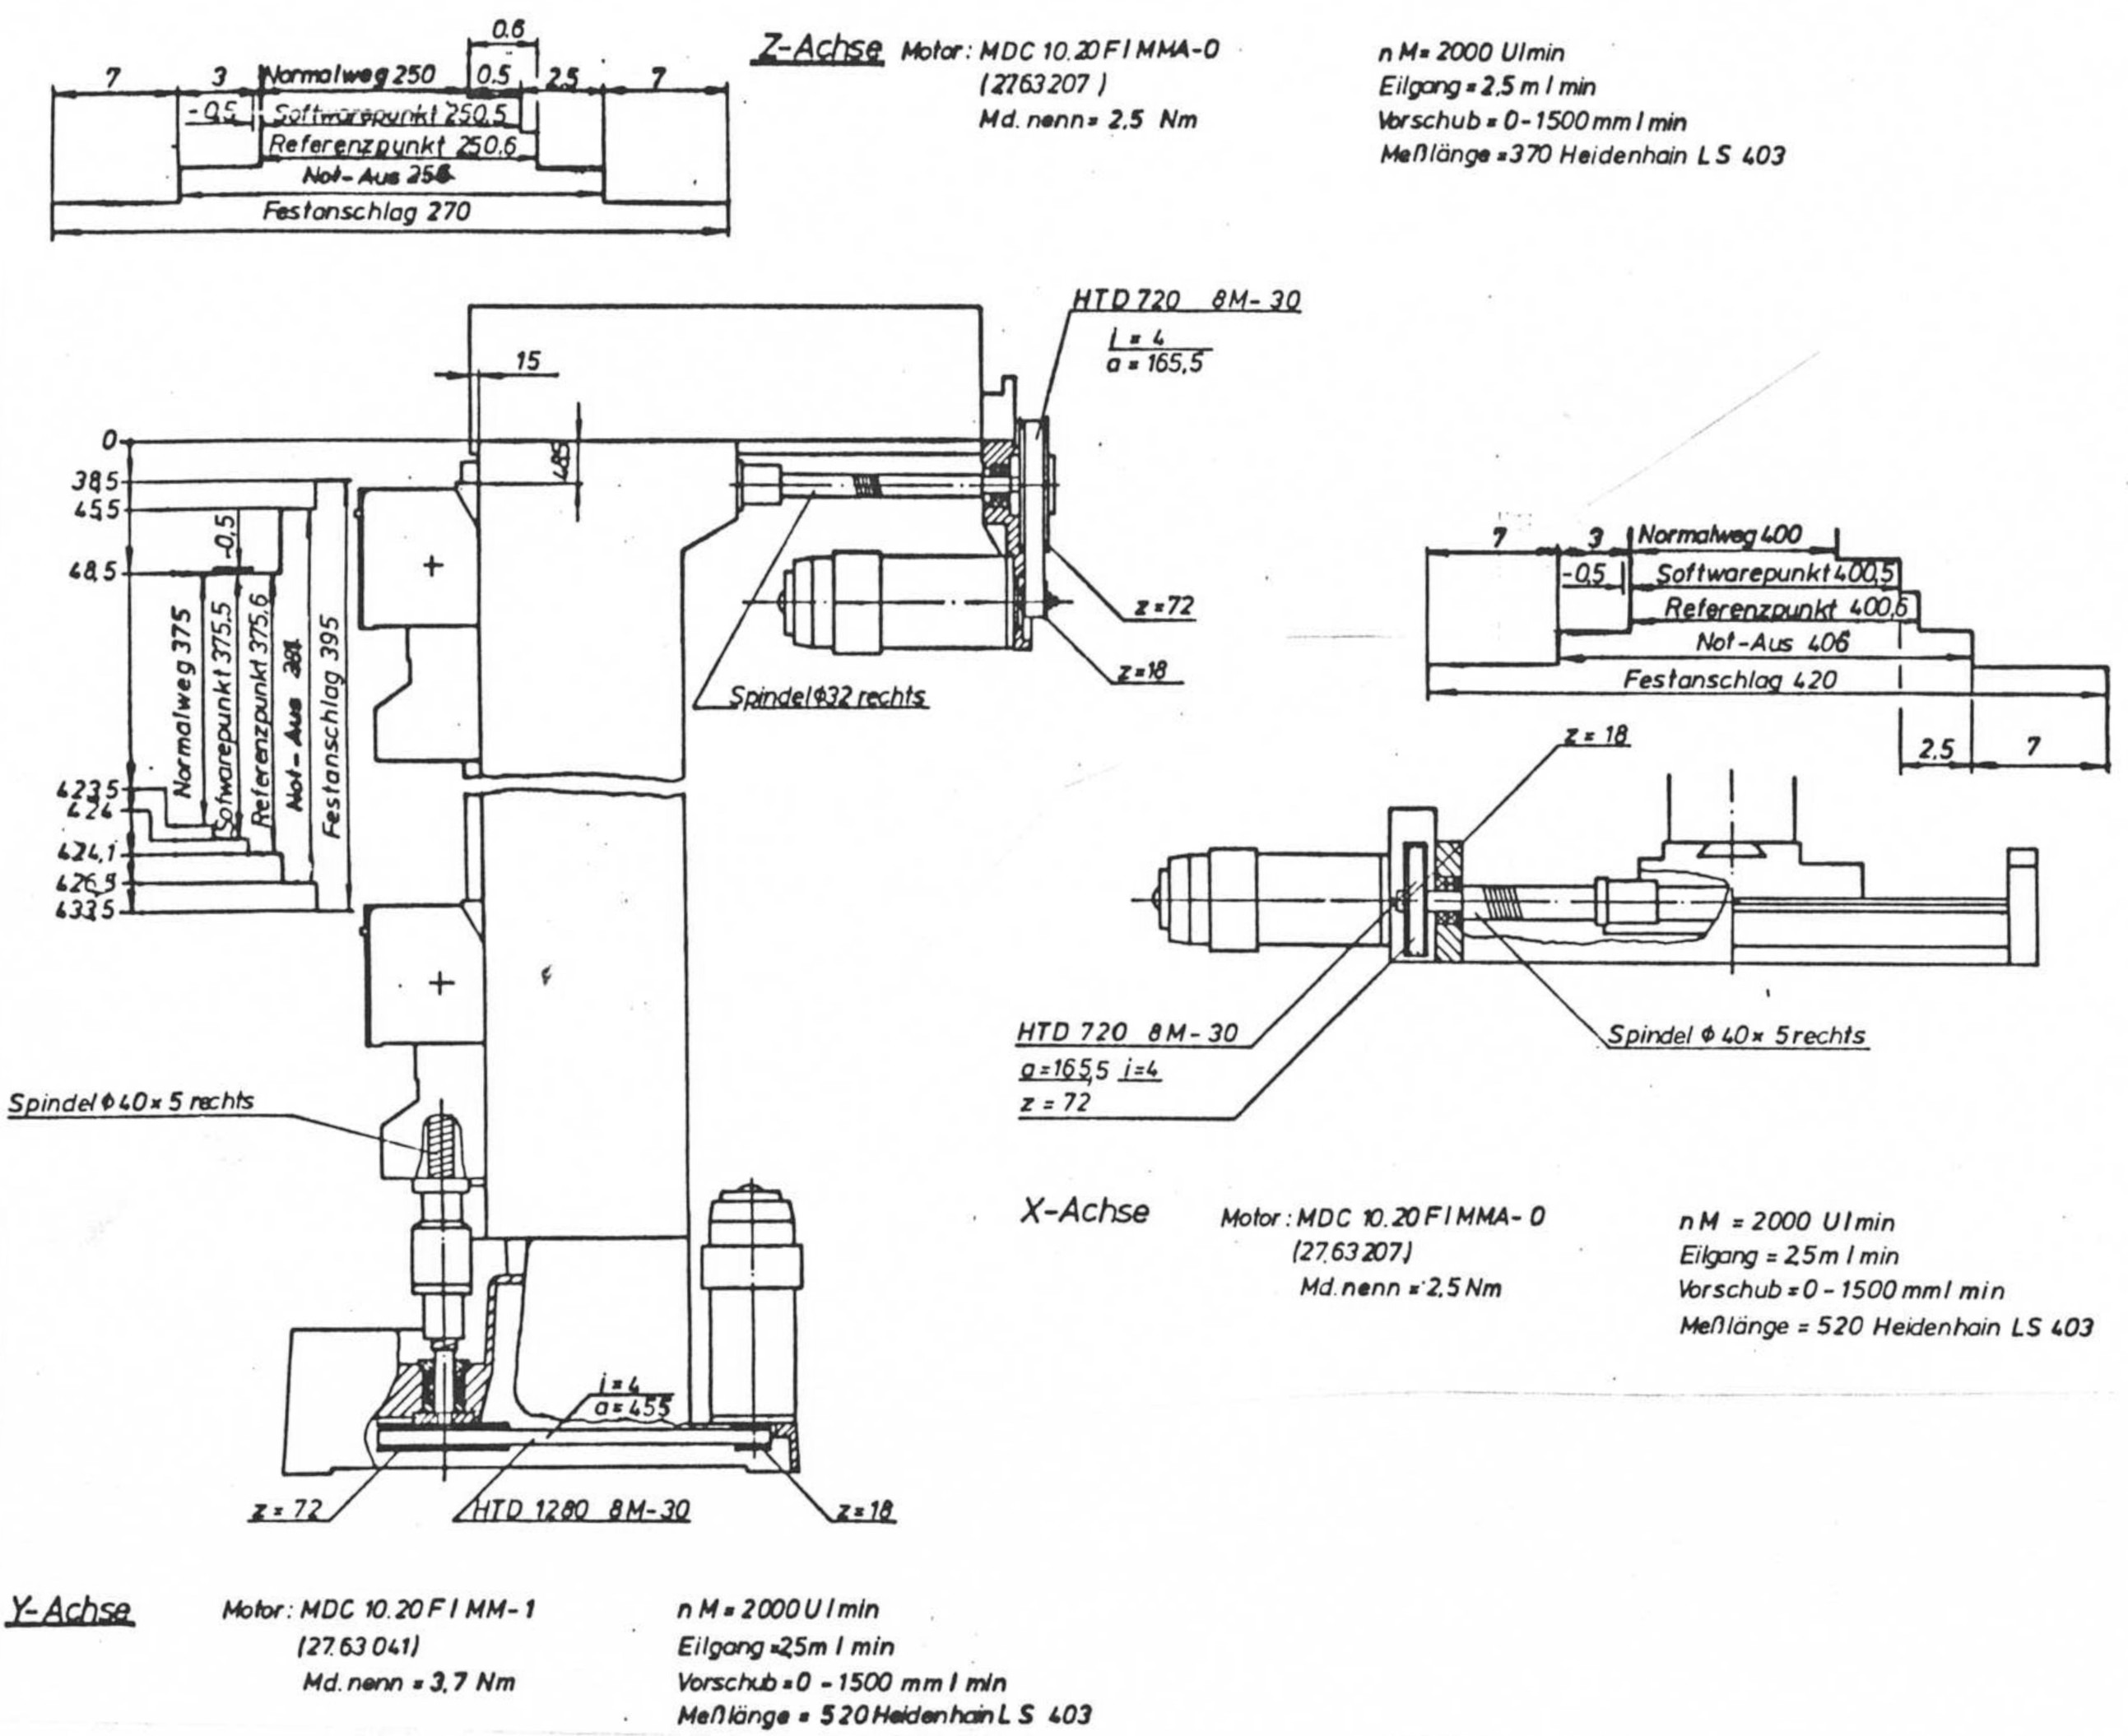
\includegraphics[angle=90,height=.9\textheight]{chapter2/gear_train_schematic.jpg}
    \end{adjustwidth}
    \label{fig:gear_train}
\end{minipage}

\sectionLikeSubsection[\texorpdfstring{14.48805/14.488111 (50/60Hz)}{14.48805-14.488111}]%
{Gear Train Schematic - Main Gearbox}

\vspace{-.5cm}

\begin{figure}[h]
    \centering
    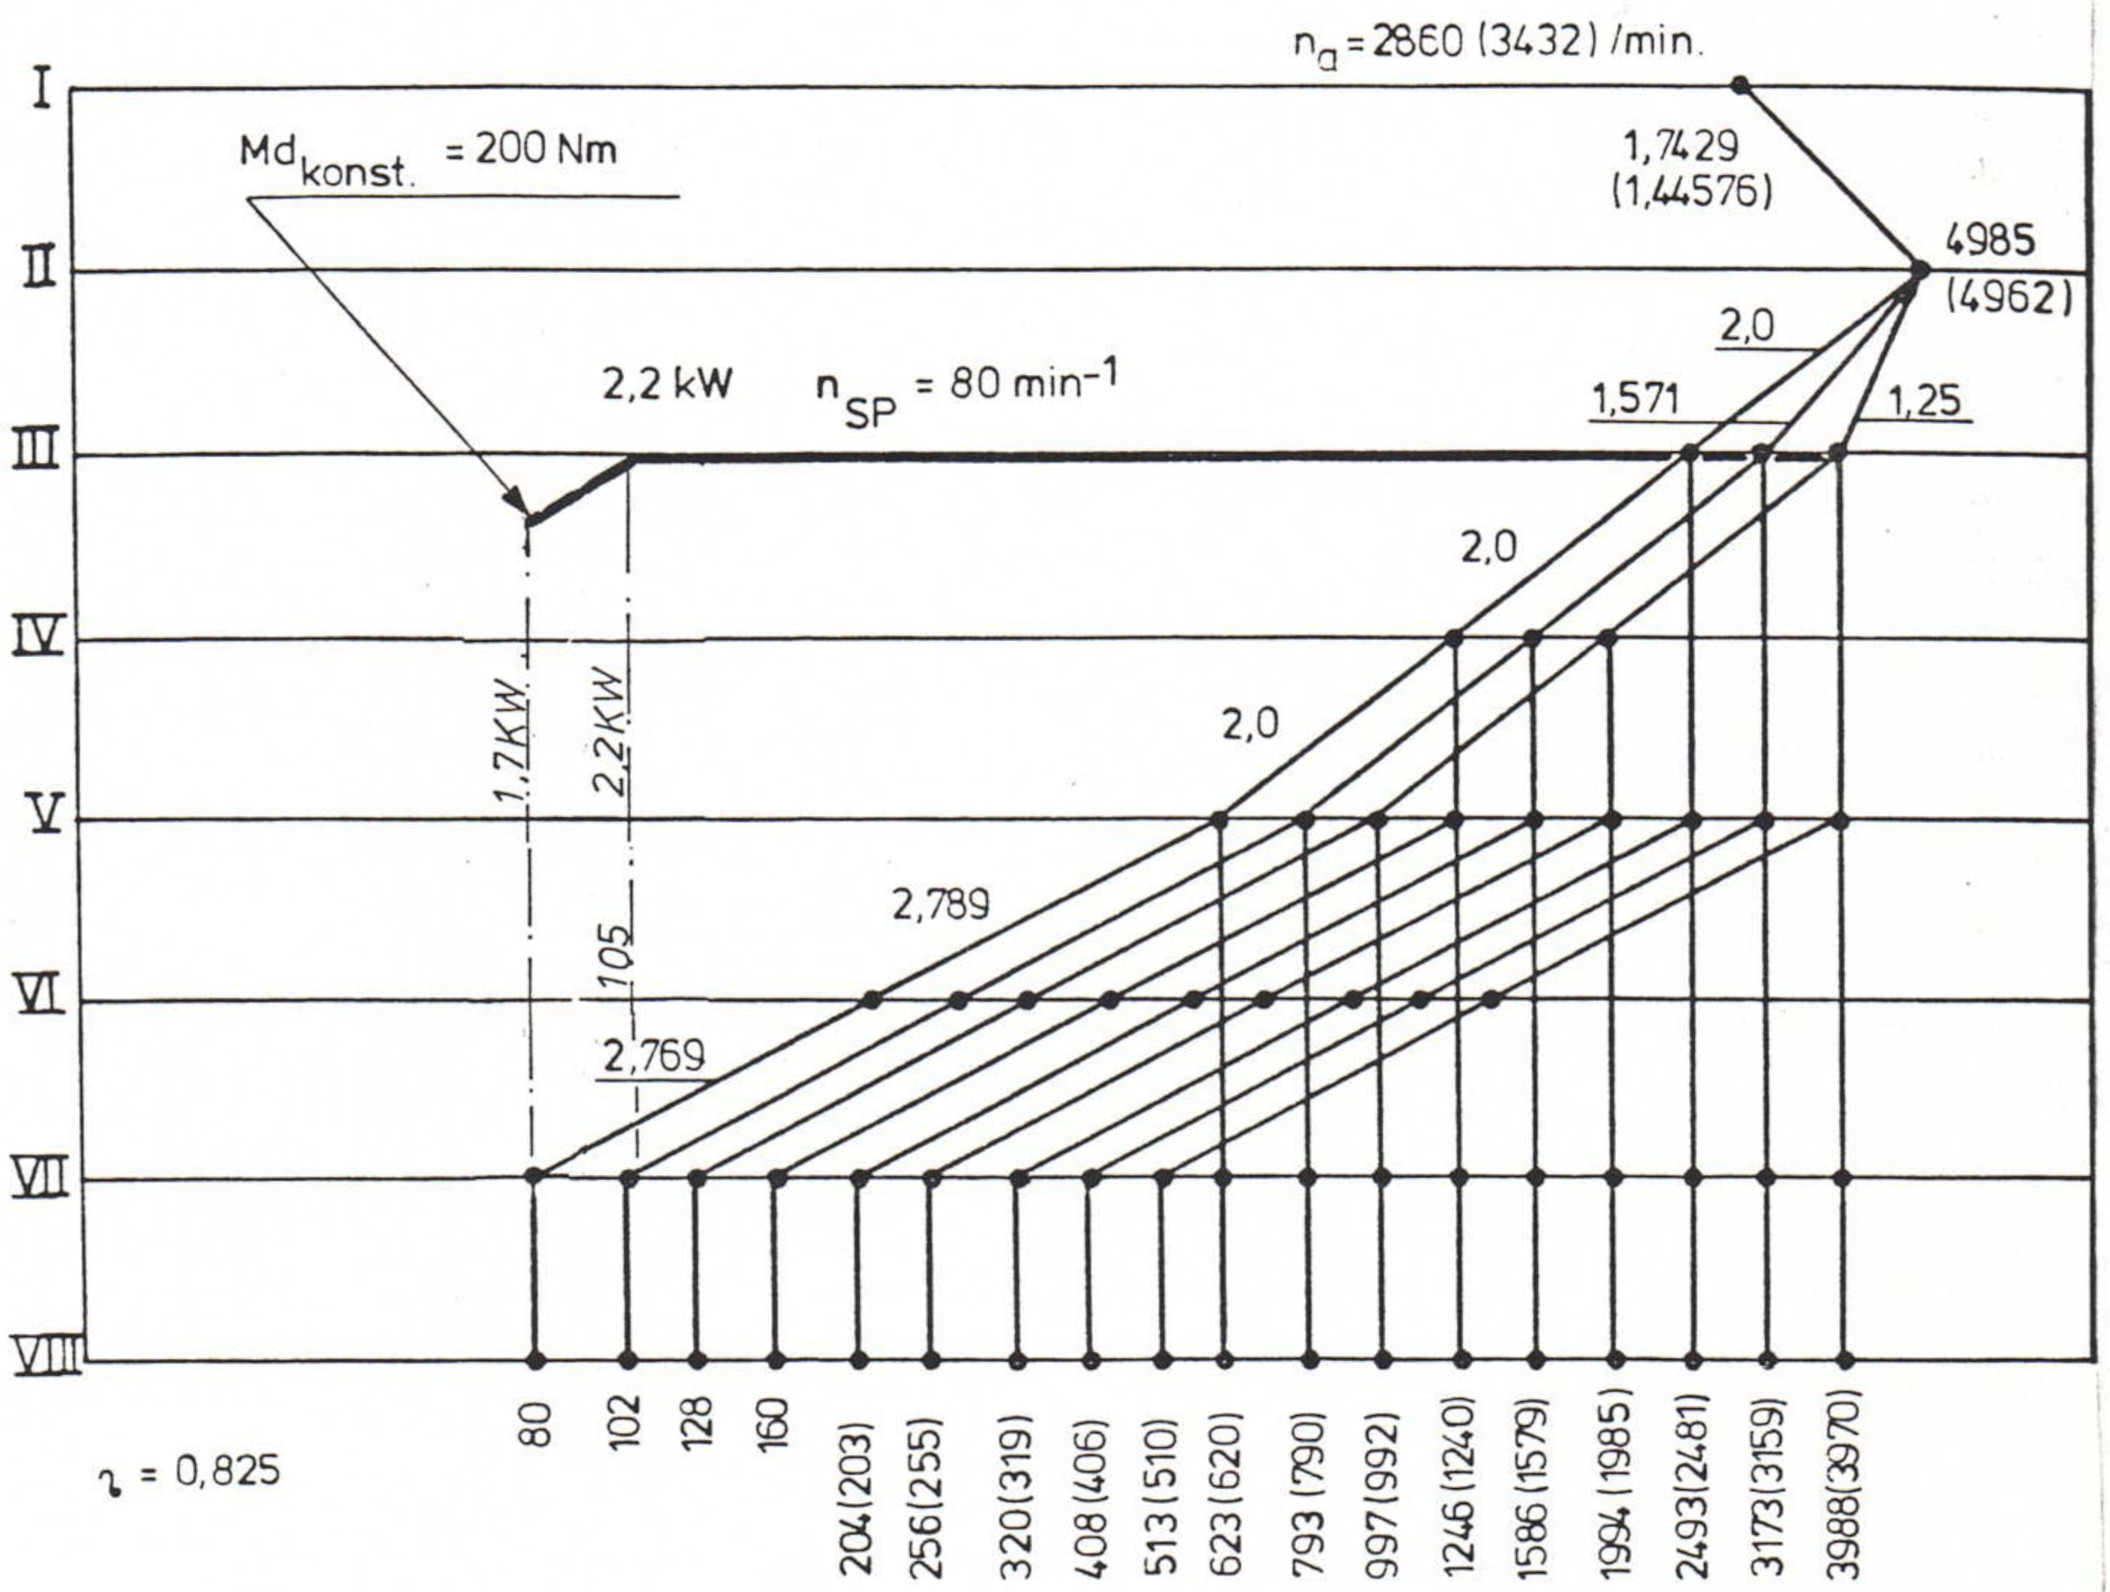
\includegraphics[width=1.05\textwidth]{chapter2/gear_train_speeds.jpg}
\end{figure}

\noindent \rule{1.08\textwidth}{0.5pt}
\footnotesize Standard Speeds: 80,100,125,160,200,250,315,400,500,630,800,1000,1250,1600,2000,2500,3150,4000
\rule{1.08\textwidth}{0.5pt}

\vspace{.5cm}

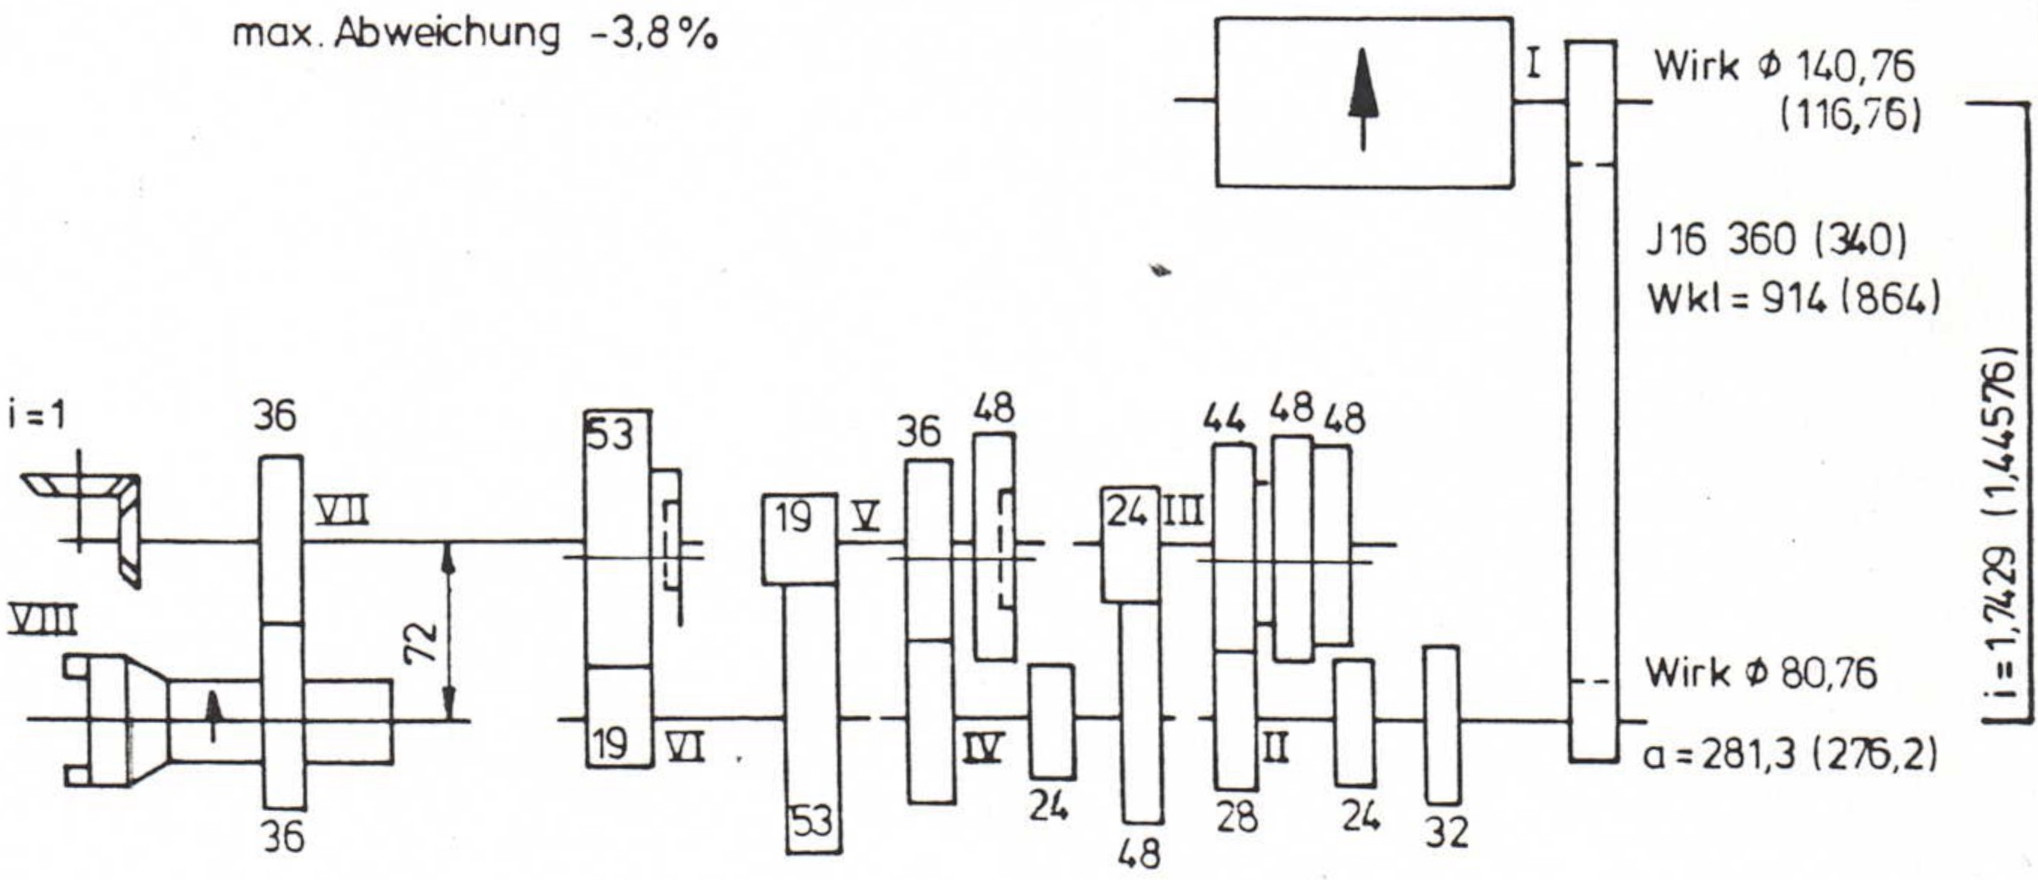
\includegraphics[width=1.02\textwidth]{chapter2/gear_train_layout.jpg}

\refstepcounter{chapter}
\addcontentsline{toc}{chapter}{Operation of the Machine}

\setsectiontitle{Function Testing / Trial Run}
\setrevision{7631}

After setting up the machine and connecting it to the power supply, a function test must be performed.

This section describes machine-specific manual operations. The operation of the control is only explained \textbf{briefly}; detailed instructions can be found in the CNC 432/10-Graphics operating manual.

\begin{itemize}
    \item Turn on the main switch on the control cabinet and wait until the \textbf{Power-On Diagnosis} appears on the screen to identify hardware errors. If no error is found, the screen displays the \textbf{Manual Mode} screen.
    
    \item Unlock all \textbf{Emergency Stop} buttons by turning them to the right.
    
    \item Press the \textbf{Hydraulics} button \raisebox{-0.4\height}{
\includegraphics[height=20pt]{chapter3/hydraulics_button.jpg}} and then press the \textbf{CLEAR} button. Repeat within 5 seconds.
    
    \item While holding the \textbf{Hydraulics} button, press the \textbf{CLEAR} button to delete error messages.
    
    \item Move the reference points of the individual axes according to the CNC 432/Graphics manual.
    
    \item Press the \textbf{TEACH IN} button.
    
    \item Enter the spindle speed under address \textbf{"S"}, following the CNC 432/10-Graphics manual (e.g., 160 min\(^{-1}\) → \texttt{S 160}) and press the \textbf{ENTER} key.
    
    \item Press the \textbf{START} button \raisebox{-0.4\height}{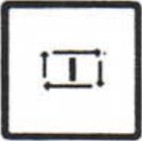
\includegraphics[height=20pt]{chapter3/start_button.jpg}}. The gearbox engages.
\end{itemize}

\notebox{NOTE}{The working spindle will not rotate until the rotation direction is entered. \enquote{M3} = Clockwise, \enquote{M4} = Counterclockwise.}

\subsection{Entering Spindle Rotation Direction}
\begin{itemize}
    \item Press the \textbf{TEACH IN} button.
    \item Enter the rotation direction under address \textbf{"M"} according to the CNC 432/10-Graphics manual.
    \item Press the \textbf{ENTER} key and the \raisebox{-0.4\height}{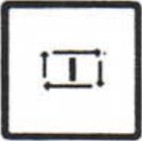
\includegraphics[height=20pt]{chapter3/start_button.jpg}} button.
\end{itemize}

\notebox{NOTE}{The working spindle rotates according to the entered direction. If the command does not execute correctly, contact MAHO service.}

\subsection{Stopping the Working Spindle via Command \textbf{"M5"}}
\begin{itemize}
    \item Press the \textbf{TEACH IN} button.
    \item Enter the stop command \textbf{"M5"} according to the CNC 432/10-Graphics manual.
    \item Press the \textbf{ENTER} key and the \raisebox{-0.4\height}{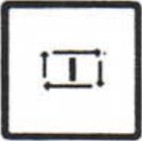
\includegraphics[height=20pt]{chapter3/start_button.jpg}} button. The working spindle stops.
\end{itemize}

\newpage

\subsection{Stopping with Function Key}

\begin{itemize}
    \item Press the \raisebox{-0.4\height}{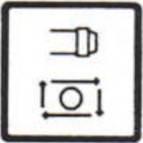
\includegraphics[height=20pt]{chapter3/stop_button.jpg}} button (feed and rotation stop immediately). If the \raisebox{-0.4\height}{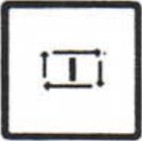
\includegraphics[height=20pt]{chapter3/start_button.jpg}} button is pressed afterward, the working spindle will restart.
\end{itemize}

\subsection{Shutting Down the System}
The entire system is shut down using the \textbf{main switch} on the control cabinet.

\subsection{Shutting Down via Emergency Stop Button}
The machine can be stopped in any operating state by pressing an \textbf{Emergency Stop (NOT-AUS)} button.

Emergency stop buttons are located on the machine control panel,on the right side of the control cabinet and on the handheld control unit.

\subsection{Releasing the Emergency Stop Button}

\notebox{WARNING}{Before unlocking, the cause of the malfunction must be resolved.}

\begin{itemize}
    \item Turn the affected Emergency Stop button to the right to release it.
    \item Restart the machine.
\end{itemize}

\subsection{Emergency Stop Limits on Machine Slides}
If the software limit fails, a mechanical switch with two cams takes over the Emergency Stop function.  
The affected slide will brake, and an alarm will be displayed on the screen.

\subsection{Restarting After an Emergency Stop}
Restarting after an Emergency Stop follows the instructions on Sheet 3.15-2.

\setsectiontitle{Manual Spindle Speed Selection}
\setrevision{859}

\setcounter{section}{3}
\setcounter{page}{2}

In case of a failure of the automatic speed selection, the spindle speed can be manually adjusted as follows:

\begin{itemize}
    \item Insert a \textbf{12 mm hex key} into the gear shift shafts (1), (3), and (5) of the main gearbox and rotate left or right until the corresponding color markers appear in the openings (2), (4), and (6), according to the speed selection table.
\end{itemize}

\begin{figure}[h]
    \centering
    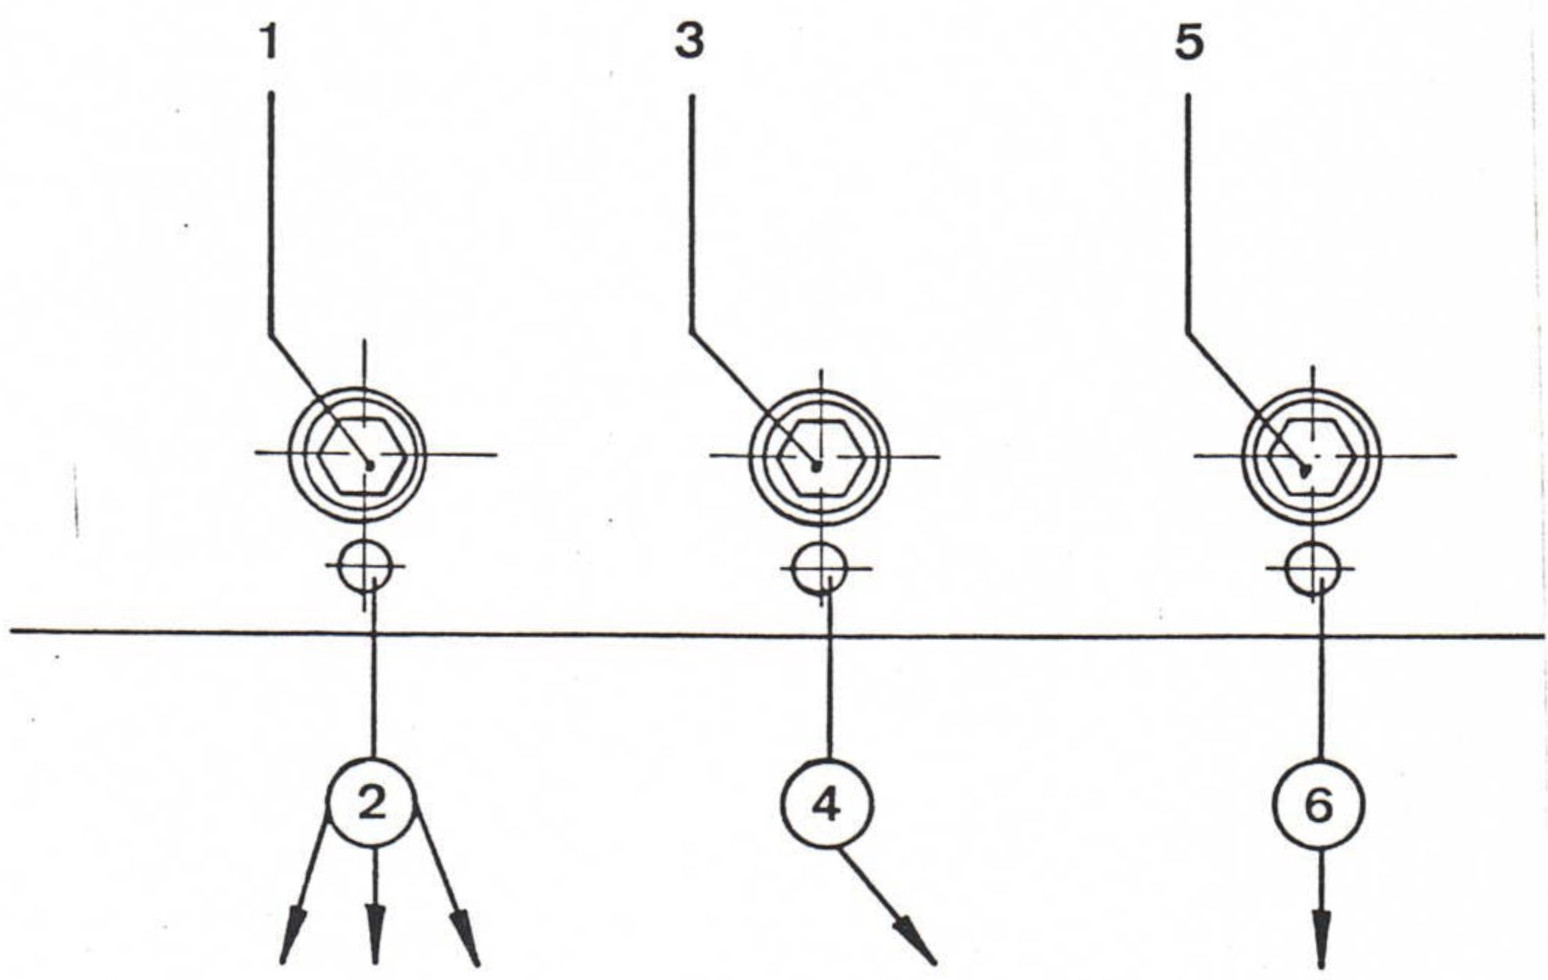
\includegraphics[width=0.8\textwidth]{chapter3/manual_spindle_speed_selection.jpg}
    \label{fig:manual_spindle_speed_selection}
\end{figure}

\begin{table}[h]
    \centering
    \renewcommand{\arraystretch}{1.3}
    \begin{tabular}{|c|c|c|c|c|}
        \hline \hline
        \textbf{} & \textbf{Silver} & \textbf{Blue} & \textbf{Green} & \textbf{Color Combination} \\
        \hline \hline
        Speed   & 80    &   Spindle & 630  & Blue - Blue  \\
        (RPM)   & 100   &   Idle    & 800  & Blue - Red   \\
                & 125   &           & 1000 & Blue - Yellow \\
                &       &           &       &               \\
                & 160   &           & 1250 & Red - Blue  \\
                & 200   &           & 1600 & Red - Red   \\
                & 250   &           & 2000 & Red - Yellow \\
                &       &           &       &               \\
                & 315   &           & 2500 & Yellow - Blue \\
                & 400   &           & 3150 & Yellow - Red  \\
                & 500   &           & 4000 & Yellow - Yellow \\
        \hline \hline
    \end{tabular}
    \label{tab:spindle_speed}
\end{table}

\setsectiontitle{Horizontal Working Spindle}

\begin{figure}[h]
    \centering
    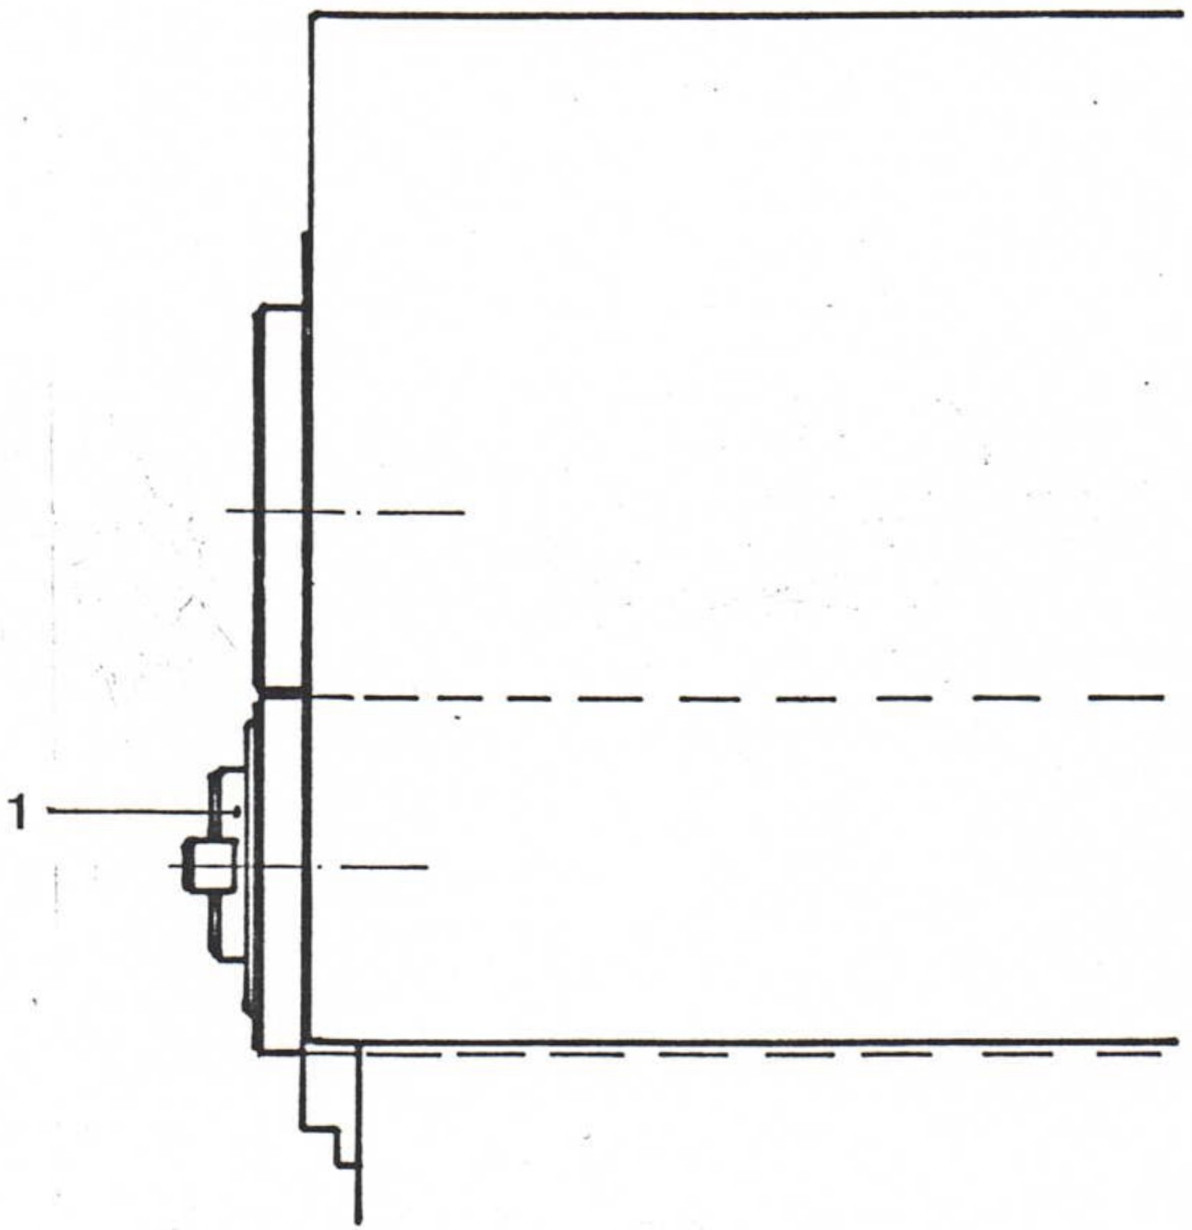
\includegraphics[width=0.7\textwidth]{chapter3/horizontal_working_spindle.jpg}
    \label{fig:horizontal_working_spindle}
\end{figure}

\textbf{1} \quad Horizontal Working Spindle

\vspace{.5cm}

\notebox{NOTE}{The spindle bearings of the working spindle are \textbf{permanently lubricated} and therefore maintenance-free.}

\setsectiontitle{Horizontal Milling with Counter Holder}
\setrevision{7631}

\begin{figure}[h]
    \centering
    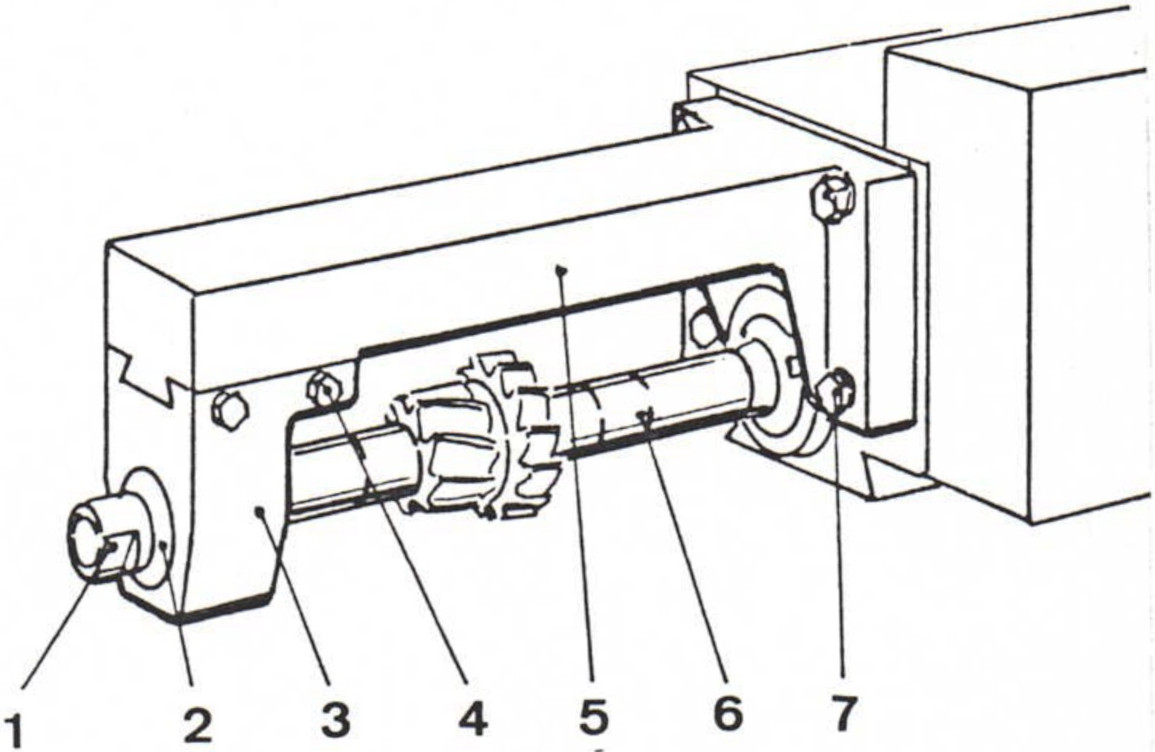
\includegraphics[width=0.8\textwidth]{chapter3/horizontal_milling_counter_holder.jpg}
    \label{fig:horizontal_milling_counter_holder}
\end{figure}

\textbf{1} \quad Clamping Nut \\
\textbf{2} \quad Guide Bushing \\
\textbf{3} \quad Cutter Arbor Bearing \\
\textbf{4} \quad Screws \\
\textbf{5} \quad Counter Holder \\
\textbf{6} \quad Cutter Arbor \\
\textbf{7} \quad Hexagon Screws

\vspace{0.3cm}

\begin{itemize}
    \item Remove the tool from the vertical working spindle (see Sheet 3.12-1).
    \item Move the vertical milling head from the working position to the resting position (see Sheet 3.08-1).
    \item Attach the counter holder (5) to the spindle stock using hexagon screws (7).
    \item Insert the cutter arbor (6), equipped with milling cutters and rings, into the horizontal working spindle and tighten (see Sheet 3.12-1).
\end{itemize}

\notebox{NOTE}{Do not install the guide bushing (2) yet.}

\begin{itemize}
    \item Slide the cutter arbor bearing (3) into the dovetail guide of the counter holder (5).
    \item Insert the guide bushing (2) into the cutter arbor bearing (3) and slide it onto the cutter arbor (6).
    \item Screw on and tighten the clamping nut (1).
    \item Secure the cutter arbor bearing (3) using screws (4).
\end{itemize}

The removal of the counter holder follows the reverse sequence.\footnotemark

\vspace{0.3cm}

\footnotetext{The conversion from horizontal to vertical machining is described on Sheet 3.07-1.}

\setsectiontitle{Horizontal to Vertical Conversion}
\setcounter{section}{7}

\begin{figure}[h]
    \centering
    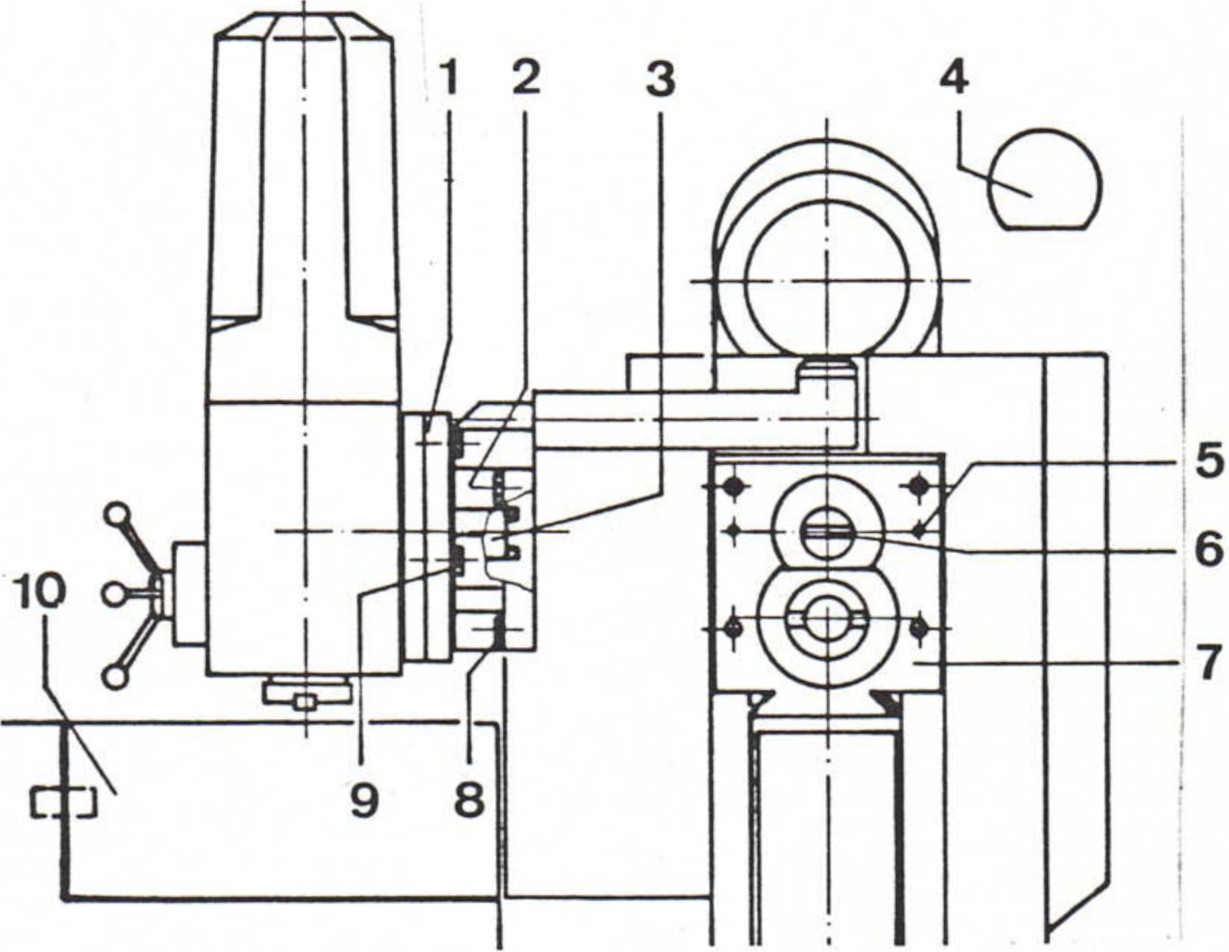
\includegraphics[width=0.8\textwidth]{chapter3/horizontal_to_vertical_conversion.jpg}
    \label{fig:horizontal_to_vertical_conversion}
\end{figure}

\vspace{0.3cm}

\begin{itemize}
    \item Remove the tool from the horizontal working spindle (see Sheet 3.12-1).
    \item Move the table down to \enquote{+Y 370} and to the left to \enquote{-X 75}.\footnotemark
    \item Open the cover flap (10) in the splash guard back panel.
    \item Set the working spindle to idle mode (S0) (see Sheet 3.01-1).
    \item Remove the protective cover (4) from the coupling component (6).
    \item Rotate the coupling components (6) and (3) so that they engage properly, aligning the marks on the spindle stock (7) and intermediate flange (2).
    \item Release the vertical milling head lock and swing it from the rear rest position to the stop at the front of the spindle stock. Press on the centering pins (5) and secure it to the spindle stock using hexagon screws (8).
    \item Close the cover flap (10).
\end{itemize}

\vspace{0.3cm}

\subsection{Swiveling the Vertical Milling Head}

\begin{itemize}
    \item Loosen the hexagon screws (9) on the intermediate flange (2).
    \item Adjust the vertical milling head according to the scale (1) to the required angle.
    \item Tighten the hexagon screws (9).
\end{itemize}

\footnotetext{Coordinates and movement directions, see Sheet 2.03-1.}

\vspace{0.3cm}

\notebox{WARNING}{When the milling head is swiveled and the splash guard cabin is installed, the X-travel is restricted.}

\setsectiontitle{Vertical to Horizontal Conversion}

\begin{figure}[h]
    \centering
    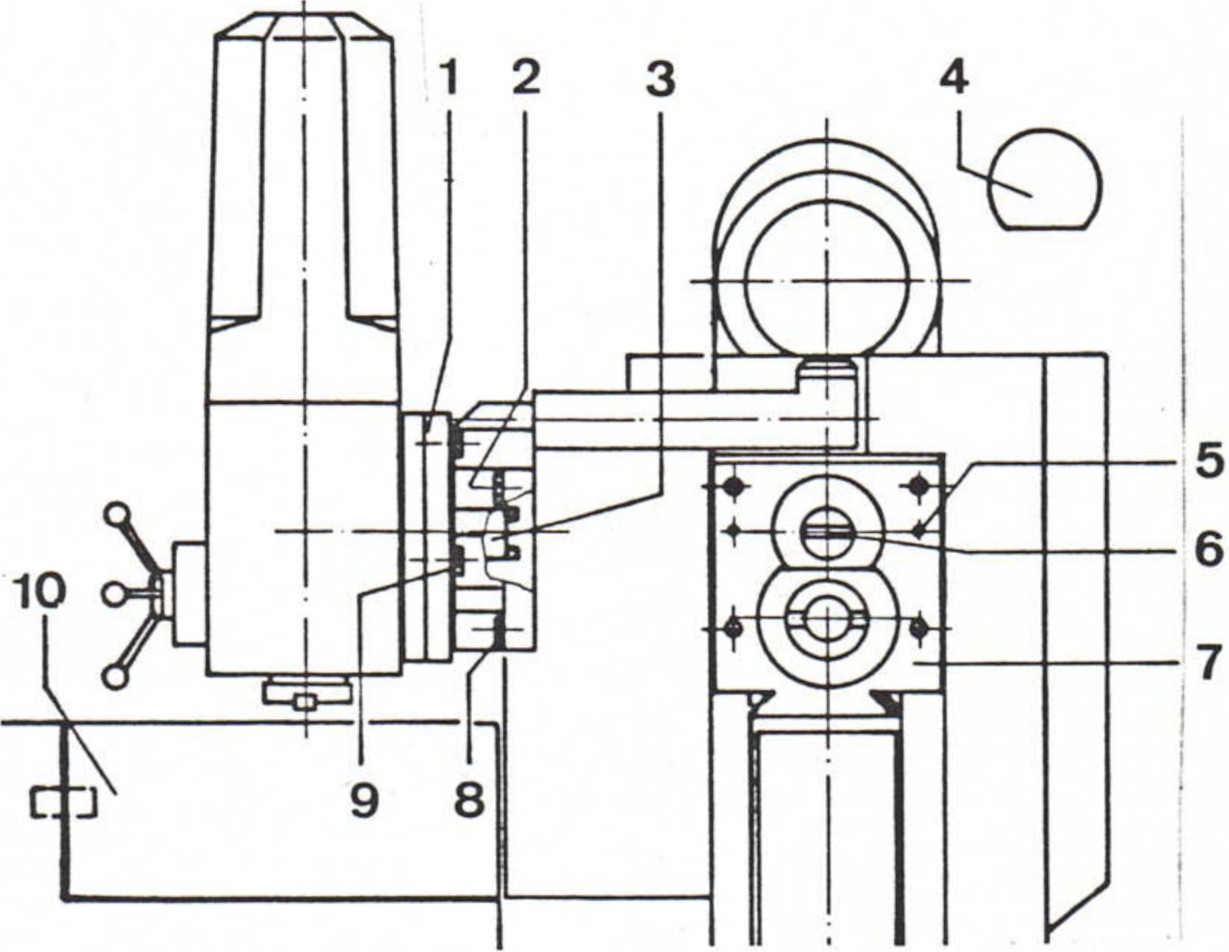
\includegraphics[width=0.8\textwidth]{chapter3/horizontal_to_vertical_conversion.jpg}
    \label{fig:vertical_to_horizontal_conversion}
\end{figure}

\begin{itemize}
    \item Remove the tool from the vertical working spindle (see Sheet 3.12-1).
    \item Move the table down to \enquote{+Y 370} and to the left to \enquote{-X 75}.\footnotemark
    \item Open the cover flap (10) in the splash guard back panel.
    \item Remove the hexagon screws (8).
    \item Push the vertical milling head away from the spindle stock (7).
    \item Swing the vertical milling head sideways into its rear resting position and lock it.
    \item Close the cover flap (10).
\end{itemize}

\footnotetext{Coordinates and movement directions, see Sheet 2.03-1.}

\setsectiontitle{Vertical Milling Head Without PVG}

\begin{minipage}{0.5\textwidth}
    \begin{enumerate}[itemsep=1pt,parsep=0pt]
        \item Quill (maximum travel = 50 mm)
        \item Vertical working spindle
        \item Scale ring for reading quill adjustment (1 tick mark = 1 mm)
        \item Handwheel for adjusting the quill
        \item Locking screw for securing the quill
        \item Clamping screw for quill locking - Allen key: 6 mm SW
    \end{enumerate}
\end{minipage}%
\begin{minipage}{0.5\textwidth}
    \centering
    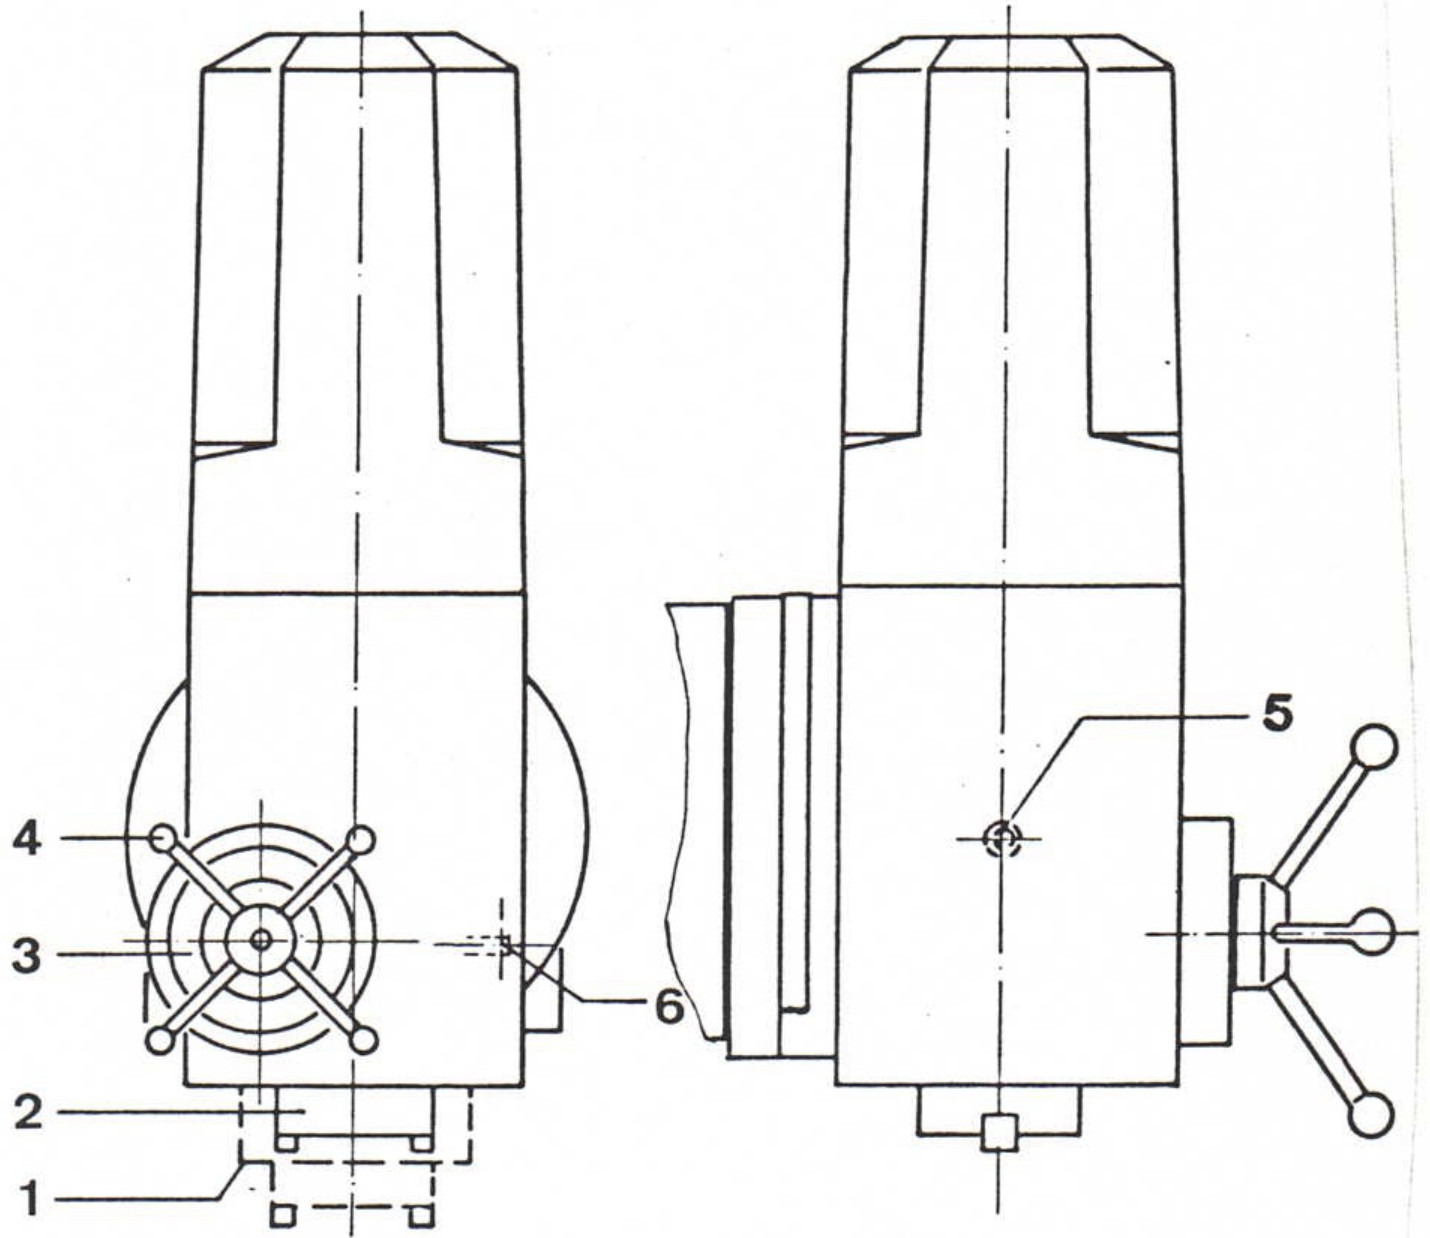
\includegraphics[width=0.9\textwidth]{chapter3/vertical_milling_head_pvg.jpg}
\end{minipage}

\vspace{0.5cm}

The quill can be additionally secured beyond normal clamping.  
This is achieved using a\\ \textbf{toothed clamping block}, which engages with the \textbf{quill rack teeth} (1) when the locking screw (5) is turned clockwise.

\vspace{0.3cm}

\notebox{WARNING}{The quill locking mechanism allows secure positioning only within a range of \textbf{0-18.5 mm travel}, in increments of \textbf{3.125 mm}.}

\vspace{0.3cm}

\notebox{NOTE}{The spindle bearings feature \textbf{lifetime lubrication}, making them \textbf{maintenance-free}.}

\vspace{0.5cm}

\subsection{What is PVG?}

The term \textbf{PVG} in this context likely refers to a \textbf{quill positioning system}, such as a \textbf{fine-feed gearbox} or a \textbf{pneumatic-assisted movement}.

\begin{itemize}
    \item Some models may feature a \textbf{Precision Feed Gearbox (Präzisions-Vorschub-Getriebe)} for \\controlled quill movement.
    \item Others may include a \textbf{Pneumatic Adjustment System (Pneumatische Verstell-Garnitur)} to aid smooth positioning.
    \item Since this model is labeled \textbf{"without PVG"}, the quill must be \textbf{manually adjusted and locked} using screws.
\end{itemize}

In short, \textbf{machines with PVG provide finer control over quill movement}, whereas \textbf{this version requires manual force} to position and lock the quill.


\setsectiontitle{Automatic Tool Clamping}
\setcounter{section}{12}

The machine's two working spindles are equipped with an \textbf{automatic tool clamping} system.

The tool is \textbf{permanently clamped} in the working spindle using \textbf{spring packs} and is released hydraulically.

A \textbf{clamping collet} secures the tool in the working spindle by engaging a \textbf{groove ring} on the cylindrical part of the tool shank. This groove ring can be retrofitted onto\\ existing tools.\footnotemark

\footnotetext[1]{Reworking the shank of standard tools is explained on Sheet 3.13-1.}

\subsection{Clamping Force for Tool Clamping (ISO 40)}

\begin{itemize}[itemsep=1pt,parsep=0pt]
   \item MAHO/OTT Clamping Collet  \dotfill 11 kN \\
   \item ISO Type B Clamping Stud \dotfill \> 9.5 kN \\
  \item  Time for Clamping/Unclamping \dotfill \> approx. 3 s
\end{itemize}

\vspace{0.5cm}

\subsection{Tool Change} \footnotemark

\footnotetext[2]{Arrangement and function of CNC control elements on the command station are described in Section 10.7 of the CNC 432 Graphics manual.}

\begin{itemize}
    \item Stop the working spindle by pressing the \textbf{Spindle/Feed Stop} button on the CNC control panel.
    \item Press the \textbf{TOOL UNCL} button to release the tool.
    \item Remove the old tool from the working spindle.
    \item Insert the new tool into the working spindle and press the \textbf{TOOL UNCL} button again to clamp it.
\end{itemize}

\notebox{WARNING}{The tool must be fully inserted before clamping is completed; otherwise, the clamping collet may be damaged.}

\vspace{0.5cm}

\begin{minipage}{0.6\textwidth}
    \centering
    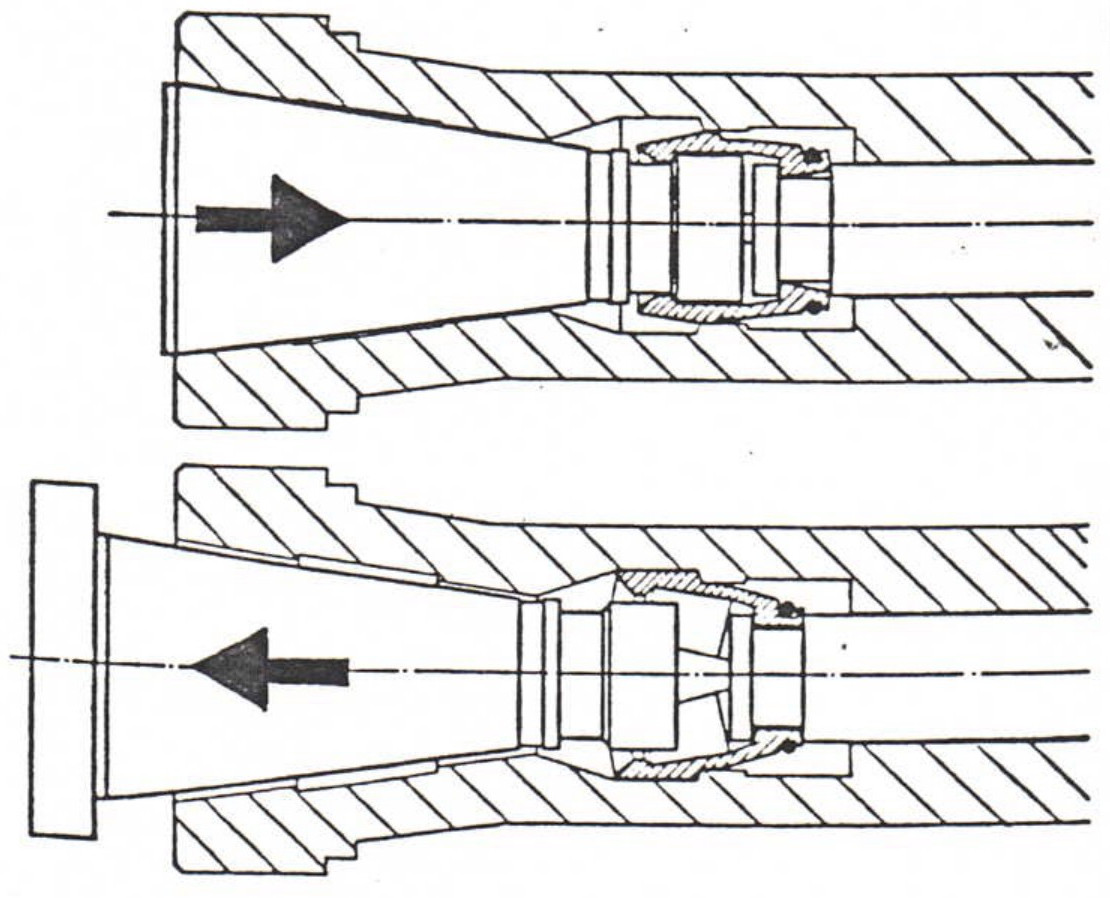
\includegraphics[width=0.9\textwidth]{chapter3/tool_clamping.jpg}
\end{minipage}%
\begin{minipage}{0.4\textwidth}
   \textbf{Clamped Condition}
    \vspace{3.2cm}\\
   \textbf{Released Condition}
\end{minipage}

\setsectiontitle{Reworking the Shank of Standard Tools}
\setrevision{859}

\textbf{MAHO/OTT, ISO 40}

\vspace{.5cm}

The ring groove on the shank of a standard tool must be modified.

\vspace{0.5cm}

\begin{minipage}{\textwidth}
    \centering
    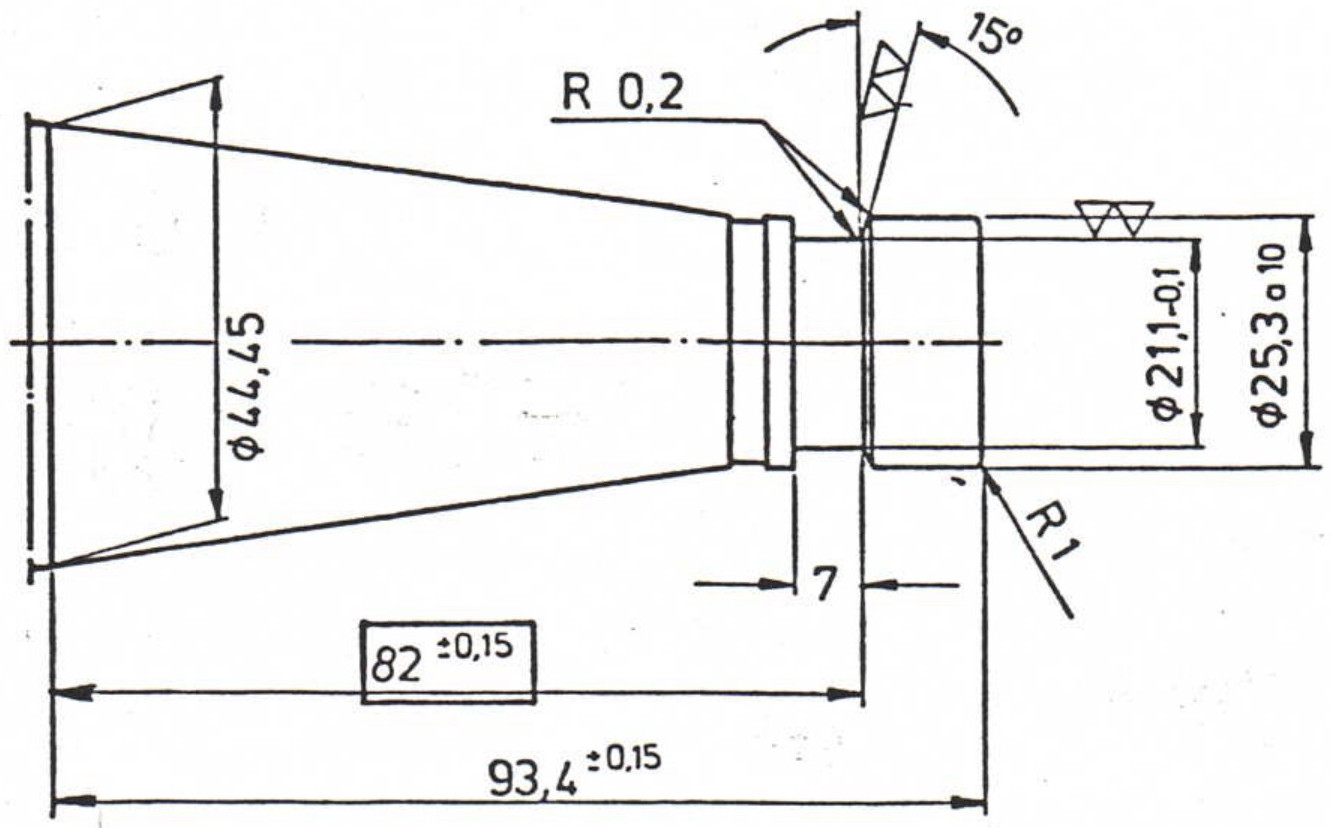
\includegraphics[width=0.8\textwidth]{chapter3/tool_shank_rework.jpg}
\end{minipage}

\vspace{0.5cm}

\textbf{Checking the Ring Groove Using the MAHO Measuring Fixture}

\begin{enumerate}[itemsep=1pt,parsep=0pt]
    \item \textbf{Mounting Bushing}
    \item \textbf{Inspection Gauge}
\end{enumerate}

\vspace{0.5cm}

\begin{minipage}{\textwidth}
    \centering
    \includegraphics[width=0.8\textwidth]{chapter3/ring_groove_inspection.jpg}
\end{minipage}

\vspace{0.5cm}

\textbf{See also Sheet 3.12-1.}

\subsection{Tool Shank According to DIN 69871 with Pull Stud ISO 7388 Type B}

\setcounter{page}{3}

\textbf{ISO 40}

\vspace{0.5cm}

\begin{minipage}{\textwidth}
    \centering
    \includegraphics[width=0.8\textwidth]{chapter3/tool_shank_iso40.jpg}
\end{minipage}

\vspace{0.5cm}

\textbf{Checking the Ring Groove Using the MAHO Measuring Fixture}

\begin{enumerate}[itemsep=1pt,parsep=0pt]
    \item \textbf{Mounting Bushing}
    \item \textbf{Inspection Gauge}
\end{enumerate}

\vspace{0.5cm}

\begin{minipage}{\textwidth}
    \centering
    \includegraphics[width=0.7\textwidth]{chapter3/ring_groove_measurement.jpg}
\end{minipage}

\vspace{0.5cm}

\textbf{See also Sheet 3.12-1.}

\setsectiontitle{Manually Resetting the Machine Carriage After an Emergency Stop}
\setrevision{7631}

\setcounter{page}{2}
\setcounter{section}{15}

If the normal travel range of the X, Y, or Z axes is exceeded due to a slip error, the machine is stopped by the \enquote{Emergency Stop} limit switch. The error \enquote{05} is displayed on the screen.

To restart the machine, the carriages must be manually moved back. This is done by rotating the motor shafts approximately 3-5 turns until the emergency stop limit switch is released.

Afterward, clear error \enquote{05} and reapproach the reference point.

\vspace{.3cm}

\notebox{WARNING}{%
Before resetting the Y-axis, open the control cabinet, hold the motor shaft using a double-ended wrench (5), then set the rotary switch \enquote{Y-Axis Brake} (on the adjustment module) to \enquote{Release}. After moving out of the emergency stop area, return the switch to \enquote{Brake Engaged}.
}

\notebox{NOTE}{%
For \enquote{Clearing Error Messages}, see the CNC control manual.
}

\textbf{Required tools from the standard accessories:}\\
(1) Hex screwdriver, (3) Square socket wrench, (5) Double-ended wrench

\vspace{2cm}

\textbf{The motor shafts are accessible at the following locations:}  

\begin{textblock*}{\textwidth}(10.5cm, 12.5cm)
\begin{itemize}
    \item \textbf{X-Axis:} After removing the cap (2).  
    \item \textbf{Y-Axis:} After removing the sheet metal cover (4) \\- under the control cabinet.  
    \item \textbf{Z-Axis:} Through the borehole in the top cover.  
\end{itemize}

\vspace{0.3cm}

\notebox{NOTE}{%
Counterclockwise rotation results in \\movement as follows:
\begin{itemize}
    \item \textbf{-X}: Table moves left.
    \item \textbf{-Y}: Support moves upwards.
    \item \textbf{-Z}: Spindle stock moves backward.
\end{itemize}
}

\end{textblock*}

\begin{minipage}{\textwidth}
    \centering
    \includegraphics[width=0.9\textwidth]{chapter3/machine_carriage_reset.jpg}
\end{minipage}

\setsectiontitle{Hydraulic Diagram}
\setcounter{section}{18}

\begin{figure}[h]
    \centering
    \includegraphics[width=.95\textwidth]{chapter3/hydraulic_diagram.jpg}
\end{figure}

\begin{textblock*}{\textwidth}(12.7cm, 9.3cm)
    \textbf{Oil Volume:} Total 2.01 l, Usable 1.3 l \\
    \textbf{Oil Type:} CL 46 DIN 51502 \\
    \textbf{Flow Rate:} $Q = 1.81 \text{ l/min}$ \\
    \textbf{Power:} $P = 0.37 \text{ kW}$ \\
    \textbf{Pump Speed:} $n = 2810 \text{ min}^{-1}$
\end{textblock*}

\begin{textblock*}{\textwidth}(7cm, 15.2cm)
    \textbf{throttle bore} \O0,5
\end{textblock*}

\vspace{1cm}

\subsection{Hydraulic Equipment List}

\begin{table}[h]
    \centering
    \begin{tabularx}{\textwidth}{|l|l|l|l|l|}
        \hline
        \textbf{Plan}   & \textbf{Ident-Nr.}    & \textbf{Description}      & \textbf{Specification}    & \textbf{Manufacturer} \\
        \textbf{Nr.}    &                       &                           &                           &                       \\
        \hline
        \hline
        0.1             & 27.70463              & Hydraulic compact unit     & N. Stückl.               & HAWE                  \\
                        &                       & SK 7611                    & 7310 700                 &                       \\
        0.2             & (in Pos.              & Pressure limiting valve    &                          & HAWE                  \\
                        & 0.1)                  &                            &                          &                       \\
        1.1             & 81.22225              & Hydraulic line             & AF4 2300 mm              & Tecalemit             \\
        1.2             & 81.22221              & Hydraulic line             & AF4 2300 mm              & Tecalemit             \\
        1.3             & 27.67898              & Clamping head, horizontal  & 95.100.366.3.2           & Ott                   \\
        1.4             & 81.15108              & Hydraulic line             & AF4 1700 mm              & Tecalemit             \\
        1.5             & 27.69738              & Clamping head, vertical    & 95.100.558.2.2           & Ott                   \\
        \hline
    \end{tabularx}
    \label{tab:hydraulic_list}
\end{table}

\newpage
\subsection{Hydraulic System}
\setcounter{page}{3}

\begin{figure}[h]
    \centering
    \includegraphics[width=0.8\textwidth]{chapter3/hydraulic_unit.jpg}
    \label{fig:maho_hydraulic_unit}
\end{figure}

\begin{enumerate}
    \item \textbf{Filler Neck} \footnotemark
    \item \textbf{Hydraulic Unit}
    \item \textbf{Transparent Container}
    \item \textbf{Oil Strainer}
\end{enumerate}

\footnotetext[1]{See Sheet \textbf{7.06-1}, \textit{"Lubrication Recommendations"}.}

\notebox{warning}{When refilling oil, ensure maximum cleanliness.  
The oil strainer must be thoroughly cleaned.}

\subsubsection{Functionality}  \footnotemark
\footnotetext[2]{Layout and function of the control station elements, see Sheet \textbf{2.04-1}.}

\textit{(See hydraulic diagram, Sheet 3.18-1)}

Pressing the illuminated push button \textbf{-3SH1-} on the control station starts the  
pump of the hydraulic unit and, within a few seconds, builds up the operating  
pressure of approximately \textbf{115 bar} required for releasing the tool clamps.  

The indicator light \textbf{-3H1-} on the control station illuminates, indicating  
that the operating pressure of the hydraulic system is present.

\setsectiontitle{Automatic Central Lubrication System}

\setcounter{section}{20}

\begin{figure}[h]
    \centering
    \includegraphics[width=0.8\textwidth]{chapter3/central_lubrication.jpg}
    \label{fig:maho_central_lubrication}
\end{figure}

% Bottom-aligned rotated labels
\begin{textblock*}{3cm}(10.8cm,4.8cm)
    {\rotatebox{90}{\textbf{Spindle Nut X-Axis}}}
\end{textblock*}

\begin{textblock*}{3cm}(11.3cm,3.85cm)
    {\rotatebox{90}{\textbf{Spindle Nut Y-Axis M8x1}}}
\end{textblock*}

\begin{textblock*}{3cm}(11.75cm,4.95cm)
    {\rotatebox{90}{\textbf{X-Surface, Bottom}}}
\end{textblock*}

\begin{textblock*}{3cm}(12.2cm,5.4cm)
    {\rotatebox{90}{\textbf{Y-Surface, Left}}}
\end{textblock*}

\begin{textblock*}{3cm}(12.65cm,5.2cm)
    {\rotatebox{90}{\textbf{Y-Guidance, Left}}}
\end{textblock*}

\begin{textblock*}{3cm}(13.55cm,5.15cm)
    {\rotatebox{90}{\textbf{Y-Surface, Right}}}
\end{textblock*}

\begin{textblock*}{3cm}(14cm,5cm)
    {\rotatebox{90}{\textbf{Y-Guidance, Right}}}
\end{textblock*}

\begin{textblock*}{3cm}(14.45cm,5.15cm)
    {\rotatebox{90}{\textbf{X-Surface, Upper}}}
\end{textblock*}

\begin{textblock*}{3cm}(14.9cm,5cm)
    {\rotatebox{90}{\textbf{X-Guidance, Upper}}}
\end{textblock*}

\begin{textblock*}{3cm}(15.35cm,5cm)
    {\rotatebox{90}{\textbf{X-Guidance, Lower}}}
\end{textblock*}

\begin{textblock*}{3cm}(10.5cm,11cm)
    {\rotatebox{90}{\textbf{\uline{Distributor on}}}}
    {\rotatebox{90}{\textbf{\uline{the Cross Slide}}}}
\end{textblock*}

% Non-rotated labels
\begin{textblock*}{5cm}(3.8cm,11.4cm)
    \textbf{Spindle head guide, right}
\end{textblock*}

\begin{textblock*}{5cm}(3.8cm,12.3cm)
    \textbf{Spindle head guide, left}
\end{textblock*}

\begin{textblock*}{5cm}(3.8cm,12.95cm)
    \textbf{Spindle Nut Z-Axis}
\end{textblock*}

\begin{textblock*}{5cm}(12cm,11cm)
    \textbf{\uline{Distributor on the Stand}}
\end{textblock*}

\newpage
\subsection{Device List}

\begin{table}[h]
    \centering
    \renewcommand{\arraystretch}{1.2}
    \begin{tabular}{|c|c|l|l|l|}
        \hline
        \hline
        \textbf{Plan} & \textbf{ID No.} & \textbf{Designation} & \textbf{Specification /} & \textbf{Manufacturer} \\
        \textbf{No.} &&&\textbf{Dimensions}& \\
        \hline
        \hline
        0.1 & 27.70580 & Gear Pump Unit & 122.049.306 220 V & Vogel \\
        0.2 & 27.51353 & Plastic Tube & 6x1,25 WWN 715-Ra & Vogel \\

        1.1 & 27.62207 & Piston Distributor with & 345 433 333 & Vogel \\
        && Dosing && \\
        1.2 & 27.51352 & Plastic Tube & 4x0,85 ERA-Pla. & Vogel \\
        1.3 & 27.52504 & Swivel Screw Connection & 504.161 & Vogel \\
        2.1 & 81.18655 & Plastic Tube & 6x1,25 WWN 715-Ra & MAHO \\

        3.1 & 27.62207 & Piston Distributor with & 345 433 333 & Vogel \\
        && Dosing && \\
        3.2 & 27.62207 & Piston Distributor with & 345 433 333 & Vogel \\
        && Dosing && \\
        3.3 & 27.51230 & Threaded Piece & 406 233 & Vogel \\
        3.4 & 27.51352 & Plastic Tube & 4x0,85 ERA-Pla. & Vogel \\
        3.5 & 27.52504 & Swivel Screw Connection & 504.161 & Vogel \\
        3.6 & 27.51725 & Swivel Screw Connection & 504.401 & Vogel \\
        3.7 & 27.52505 & Swivel Screw Connection & 504.411 & Vogel \\
        \hline
        \hline
    \end{tabular}
\end{table}

\newpage
\setrevision{8627}

\begin{figure}[h]
    \centering
    \includegraphics[width=0.8\textwidth]{chapter3/lubrication_unit.jpg}
\end{figure}

\begin{enumerate}
    \item Central lubrication unit
    \item Green indicator light \textit{"Operation"}
    \item Pressure connection R 1/4"
    \item Cover
    \item Red indicator light \textit{"Fault"}
    \item Oil filling opening with built-in sieve
    \item Push button for manually triggering the lubrication pulse
    \item Transparent container
    \item Mounting plate
    \item Fan wheel
    \item Float switch
\end{enumerate}

\notebox{WARNING}{%
    The values set under machine constants MC 758, 759, 767, and 768 must not be changed.
}

Pump runtime until pressure build-up, plus 15 s overrun time (MC 768 = 15).

A fault signal occurs if the pressure build-up fails 60 s after the pump starts.

\newpage

\subsection*{Functionality}

The motion-independent automatic central lubrication ensures an even supply of oil to all sliding surfaces and moving elements of the machine.

Through a lubrication pulse, the pump of the central lubrication unit (1) starts and pumps oil into the pipeline system until the necessary pressure for oil supply is reached. Once this pressure is achieved, a pressure monitor switches the pump off.

During the lubrication process, the green indicator light (2) \textit{"Operation"} is illuminated.

Lubrication pulses are triggered:

\begin{enumerate}
    \item With each machine start, by pressing the illuminated push button -3SH1- on the control station.\footnotemark
    \item When the machine is running without any axis movement, after every 8 hours. (MC 767 = 480).
    \item When the movement of one or multiple axes, with or without interruptions, lasts longer than 16 minutes. (MC 758 = 16).
    \item When an axis starts moving and the last lubrication pulse was more than 32 minutes ago. (MC 759 = 32).
\end{enumerate}

If lubrication fails, the pressure monitor causes the shutdown of the hydraulics and feed drive. The red indicator light (5) \textit{"Fault"} illuminates, and the machine is automatically stopped through the emergency stop circuit.

\subsection*{Restarting the Machine after Lubrication Failure}

\begin{itemize}
    \item Check the oil level in the transparent container (8) and refill if necessary via the filling opening (6).\footnotemark
    \item Check the main line between the central lubrication unit (1) and oil distributors (see sheet 3.20-1) for leaks.
\end{itemize}

\subsection*{After Resolving the Malfunction}

\begin{itemize}
    \item Press the illuminated push button -3SH1- on the control station.\footnotemark[1]
    \item The indicator light -3H1- illuminates.
\end{itemize}

\notebox{note}{%
    After a long downtime of the machine, additional lubrication pulses can be triggered if necessary by pressing the push button (7) on the central lubrication unit. The indicator light (2) \textit{"Operation"} must light up and must turn off at the end of the lubrication process. This must be done before \textbf{"PROGRAM START"}, as otherwise, the program sequence would be interrupted by \textit{"Spindle and feed stop"}.
}

\footnotetext[1]{Arrangement and function of the control elements on the control station, see sheet 2.04-1.}
\footnotetext[2]{See sheet 7.06-1 \textit{"Lubricant Recommendations"}.}

\subsection{Hydraulic Plan and Circuit Diagram}
\setrevision{859}

\subsubsection*{Hydraulic Plan}

\begin{minipage}{0.65\textwidth}
    \includegraphics[width=.8\linewidth]{chapter3/hydraulic_plan.jpg}
\end{minipage}%
\begin{minipage}{0.35\textwidth}
    \begin{itemize}
        \item[1] Gear Pump Unit
        \item[2] Hydraulic Valve
        \item[3] Pressure Relief Valve
        \item[4] Pressure Switch
        \item[5] Float
    \end{itemize}
    
    \vspace{1em}
    \textbf{Pump Output:} 0.1 l/min \\
    \textbf{Max Connection Volume:} 18 cm\textsuperscript{3}
\end{minipage}

\vspace{2cm}

\subsubsection*{Circuit Diagram (Shown for 220V)}

\begin{minipage}{0.65\textwidth}
    \includegraphics[width=.8\linewidth]{chapter3/hydraulic_circuit_diagram.jpg}
\end{minipage}%
\begin{minipage}{0.35\textwidth}
    \begin{itemize}
        \item[\textbf{L1}] Operating Indicator Lamp 24V=
        \item[\textbf{L2}] Fault Indicator Lamp 24V=
        \item[\textbf{Ws}] Float Switch
        \item[\textbf{Ds}] Pressure Switch
        \item[\textbf{IG 36}] Control Device
        \item[\textbf{DK}] Push Button
        \item[\textbf{Ms}] Machine Main Switch
    \end{itemize}
\end{minipage}

\vspace{1cm}

\begin{tabular}{ll}
    Total Power Consumption: & \textbf{100 W} \\
    Motor Power: & \textbf{20 W} \\
    Motor Pump Speed: & \textbf{2600 min\textsuperscript{-1}}
\end{tabular}

\setsectiontitle{Coolant Lubrication System}
\setrevision{7631}

\setcounter{section}{22}

\begin{figure}[h]
    \centering
    \includegraphics[width=0.8\textwidth]{chapter3/coolant_system.jpg}
\end{figure}

\begin{enumerate}
    \item Coolant reservoir (Capacity approx. 80 l)\footnotemark
    \item Coolant pump -2M1- (Flow rate 56 l/min at 2°E/50°C)\footnotemark
    \item Removable cover plate
    \item Connecting pipe between pump -2M1- and spindle head
    \item Adjustable pipe with nozzle for coolant supply to the tool\footnotemark
    \item Valve for adjusting the coolant flow
\end{enumerate}

\footnotetext[1]{To avoid foam formation, the coolant reservoir should be kept as full as possible.}
\footnotetext[2]{The coolant pump is switched on using program code \texttt{M8} and off using \texttt{M9} on the CNC control panel (see CNC manual \#32).}
\footnotetext[3]{For coolant specifications, see sheet 7.07-1.}

\setsectiontitle{Splash Protection}

\setcounter{section}{24}

The splash protection consists of a chip tray (6), which is firmly attached to the vertical clamping table and moves along the X-axis.

\begin{itemize}
    \item Two frames with safety glass (4) are attached to this chip tray (6) using hinges and can be folded down. They are connected by locks (2). The right side panel (5) can be unfolded and lowered.
    \item The rear splash guard (3) is fixed to the cross support and moves along the Y-axis.
    \item When switching from horizontal to vertical machining, the flap (1) is opened.
\end{itemize}

\notebox{Warning}{The reconfiguration may only be performed in the position \texttt{+Y 370 / -X 75} of the cross support. When not in use, the vertical milling head must be precisely fixed in its resting position (see Sheet 3.07-1 / 3.08-1).}

To empty the chip tray, the bottom flap (7) must be opened using a control cabinet key. The screens in the table and the chip tray should be cleaned as needed. Use only household cleaning agents to clean the safety glass panes.

\vspace{.5cm}

\notebox{Warning}{When using a swiveled milling head, operation is only possible with a reduced X-axis travel to avoid collision hazards.}

\begin{figure}[h]
    \centering
    \includegraphics[width=\textwidth]{chapter3/splash_protection.jpg}
\end{figure}

\refstepcounter{chapter}
\addcontentsline{toc}{chapter}{Work Tables}

\setsectiontitle{Fixed Angle Table}
\setrevision{10514}

\subsection*{Application}
The fixed angle table has a rectangular shape and is used to hold bulky workpieces during machining operations that do not require an angular adjustment of the workpiece.

The fixed angle table is fastened to the machine’s vertical clamping table using T-slot nuts and hex bolts.

\subsection*{Technical Data}

\begin{itemize}
   \item \textbf{Clamping surface} \dotfill 800 x 250mm
   \item \textbf{Number of T-slots (14 H7)} \dotfill 4
   \item \textbf{Distance between T-slots} \dotfill 63mm
   \item \textbf{Weight (approx.)} \dotfill 100kg
   \item \textbf{Maximum table load (incl. workpiece and clamping tools)} \dotfill 200kg
\end{itemize}

\newpage
\subsection{Working Area Dimensions}
\setrevision{75628}

\vspace{3cm}

\begin{center}
    \includegraphics[width=.7\textwidth]{chapter4/fixed_angle_table_dimensions.jpg}    
\end{center}

\setsectiontitle{Universal Built-in Rotary Table}
\setrevision{859}

with ROD Encoder

\setcounter{section}{3}

\subsection*{Application}

The universal built-in rotary table is used for holding heavy and large workpieces during complex spatial machining operations that require high geometric precision.

To adjust the spatial angle, the table can tilt around both its transverse and longitudinal axes by ±30°, and the table plate can rotate 360°.

The table is equipped for indirect dividing.

The table plate is manually clamped.

\subsection*{Technical Data}

\begin{itemize}
   \item \textbf{Clamping surface} \dotfill 550 x 280mm
   \item \textbf{Centering bore} \dotfill 30 H7mm
   \item \textbf{Number of T-slots (14 H7)} \dotfill 4
   \item \textbf{Distance between T-slots} \dotfill 63mm
   \item \textbf{Tilting range around transverse axis} \dotfill ±30°
   \item \textbf{Tilting range around longitudinal axis} \dotfill ±30°
   \item \textbf{Rotational range of table plate} \dotfill 360°
   \item \textbf{Encoder with digital display, resolution} \dotfill 0.001°\footnotemark
   \item \textbf{Indirect dividing using handwheel:}
   \begin{itemize}
       \item Overall gear ratio \dotfill 90:1
       \item One full turn of handwheel \dotfill 4°
       \item One scale division on table \dotfill 20'
   \end{itemize}
   \item \textbf{Maximum table load (incl. workpiece and clamping tools)} \dotfill 150kg
   \item \textbf{Weight (approx.)} \dotfill 75kg
\end{itemize}

\footnotetext{Not included in versions without ROD.}

\newpage
\setrevision{7631}

\begin{figure}[h]
    \centering
    \includegraphics[width=0.8\textwidth]{chapter4/universal_rotary_table.jpg}
\end{figure}

\begin{enumerate}
    \item \textbf{Clamping plate}
    \item \textbf{Clamping screws for securing the console to the clamping plate}
    \item \textbf{Scale for reading the swivel angle of the console} (1 division = 20')
    \item \textbf{Square drive for swiveling the console around the transverse axis}
    \item \textbf{Hex bolts and T-slot nuts for securing the clamping plate} to the machine's vertical clamping table
    \item \textbf{Square drive for swiveling the swivel section around the longitudinal axis}
    \item \textbf{Console}
    \item \textbf{Scale for reading the swivel angle of the swivel section} (1 division = 10')
    \item \textbf{Handwheel drive for indirect dividing according to the table scale} (1 full turn = 4°)
    \item \textbf{Table plate, rotatable by 360°}
    \item \textbf{Scale for reading the rotation angle of the table plate} (1 division = 20')
    \item \textbf{Nuts for securing the table plate to the swivel section}
    \item \textbf{Swivel section}
    \item \textbf{Clamping screws for securing the swivel section in the console}
\end{enumerate}

\newpage

\begin{figure}[h]
    \centering
    \includegraphics[width=0.8\textwidth]{chapter4/universal_rotary_table_operation.jpg}
\end{figure}

\begin{enumerate}
    \item[16] \textbf{Clamping lever for securing the eccentric bushing} of the indexing worm.
    \item[17] \textbf{Eccentric bushing for engaging the indexing worm externally} for indirect dividing.
\end{enumerate}

\subsection*{Working with the Universal Built-in Rotary Table}
\begin{itemize}
    \item Before swiveling the table around its horizontal transverse axis, all clamping screws (2) must be loosened.
    \item Before swiveling the table around its horizontal longitudinal axis, all clamping screws (14) on both sides of the console must be loosened.
    \item When performing indirect dividing, the handwheel (9) must always be rotated in the same direction to eliminate any influence of backlash in the dividing gearbox on the indexing accuracy.
    \item The machine spindle must be stopped before each indexing operation.
    \item After each indexing operation, the table plate (10) must be secured again by tightening the nuts (12).
\end{itemize}

\newpage
\subsection*{Indirect Dividing Using Scale Ring}

\begin{itemize}
    \item Loosen the \textbf{nuts (12)} securing the table plate (10).
    \item Loosen the \textbf{clamping lever (16)} and rotate the \textbf{eccentric bushing (17)} to the right until the indexing worm is engaged, then retighten the clamping lever (16).
    \item Rotate the \textbf{handwheel (9)} to set the required rotation angle of the \textbf{table plate (10)} according to the \textbf{scale (11)}.
    \item Retighten the \textbf{nuts (12)}.
\end{itemize}

\notebox{NOTE}{Adjustment operations for the universal built-in rotary table are described in Section 7 of the operator’s manual.}

\subsection*{Lubrication / Maintenance}
\begin{itemize}
    \item Every 200 operating hours, lubricate the three grease nipples with slideway oil \textbf{"GULP 68"}.
\end{itemize}

\begin{figure}[h]
    \centering
    \includegraphics[width=0.8\textwidth]{chapter4/universal_rotary_table_lubrication.jpg}
\end{figure}

\newpage
\subsection{Work Area Dimensions}
\setrevision{5628}

\begin{figure}[h]
    \centering
    \includegraphics[width=0.75\textwidth]{chapter4/universal_rotary_table_dimensions.jpg}
\end{figure}

\setsectiontitle{Angle Adjustment Display for B-Axis}
\setrevision{859}

For working with the ROD measurement system, it is necessary to convert the commonly used angular minutes and seconds from technical drawings into decimal values.

\subsection*{Conversion}
\[
\frac{\text{min.}}{60} + \frac{\text{sec.}}{3600} = 0,\dots^{\circ}
\]

The angle position is displayed on the \textbf{CNC 432 screen} with a resolution of $0.001^{\circ}$.

\subsection*{Examples}
\begin{itemize}
    \item \textbf{Example 1:} $18^{\circ} 36' 24'' = 18.606^{\circ}$
    \item \textbf{Example 2:} $63^{\circ} 06' 49'' = 63.113^{\circ}$
    \item \textbf{Example 3:} $203^{\circ} 58' 03'' = 203.967^{\circ}$
\end{itemize}

A fixed reference point in the ROD measuring system enables precise alignment of the workpiece and the restoration of the workpiece reference point after an interruption.

Before starting work, the reference point’s position should be determined based on the T-slots aligned parallel to the X-axis or Z-axis and noted separately.\footnotemark

\subsection*{Procedure}
\begin{itemize}
    \item Set the machine constant \textbf{C 75} to \textbf{0}, making the reference point and zero point identical.
    \item Move to reference points X, Y, Z. Move the rotary table with the hand crank until the display \textbf{B-RP} disappears. The text \textbf{READ-OUT} remains displayed.
    \item Rotate the table to the desired position. Ideally, the T-slots should be parallel to the X-movement.
    \item Enter the displayed \textbf{B} value on the screen into constant \textbf{C 75} with reversed signs (positive becomes negative and vice versa). This shifts the NP (new position) by the entered C 75 value from the RP (reference point).
    \item Move back to reference points X, Y, Z and drive the rotary table with the hand crank to \textbf{0}.
    \item After a power failure, only reference points X, Y, and Z need to be re-referenced. If B was also active, it must be referenced first, otherwise, X, Y, and Z will not be released.
\end{itemize}

\footnotetext{See the separate operating instructions for CNC 432 graphics.}

\refstepcounter{chapter}
\addcontentsline{toc}{chapter}{CNC Control}

\section{Linear Measurement System}

\subsection*{The Linear Measurement Systems}
The machine is equipped with three digital incremental linear measurement systems for precise positioning along the X, Y, and Z axes.\footnotemark[1]

The resolution of these measurement systems, i.e., the smallest detectable absolute path unit, is 0.001 mm.

The linear measurement systems are fully encapsulated and mounted directly on the linear guides of the machine slides. This ensures that the measured values correspond to the actual positions between the tool and the workpiece.

\notebox{warning}{The linear measurement systems of the machine require no maintenance.}

\subsection*{Functionality of the Linear Measurement System}
A precision glass scale, which serves as the measuring body, moves along with the machine slide relative to a photoelectric scanning head with an opposing light source. As the scanning head moves, periodic light fluctuations occur, which are converted into sine waves by a silicon photodiode.

The sine signals are shaped into square-wave pulses and electronically processed so that each displacement of the scale by 0.001 mm results in an increment of the linear measurement system, producing either a forward or backward counting pulse. By correctly counting these pulses from a freely definable reference point, the actual travel distance is determined.

Additionally, the precision glass scale is equipped with a reference mark that serves as the absolute reference point of the linear measurement system.

\footnotetext[1]{Coordinate axes, see sheet 2.03-1.}

\refstepcounter{chapter}
\addcontentsline{toc}{chapter}{Accessories}

\section{High-Speed Milling Spindle}

\setcounter{section}{2}

\subsection*{Application}
The high-speed milling spindle can be used in both the horizontal working spindle and the vertical working spindle of the machine.

\subsection*{Technical Data}
\begin{itemize}
    \item \textbf{Machine spindle taper} \dotfill ISO 40
    \item \textbf{Milling spindle internal taper} \dotfill ISO 30
    \item \textbf{Planetary gear ratio} \dotfill 1:4
    \item \textbf{Speed range} \dotfill 200-8000 RPM\footnotemark[1]
\end{itemize}

\subsection*{Anti-Rotation Protection}
\begin{itemize}
    \item The housing of the high-speed milling spindle is secured against rotation using a holding bracket (2) and a support rod (1).
    \item The support rod is fastened using a nut (3) at the required distance in the longitudinal slot of the holding bracket.
    \item The guide hole for mounting the support rod is located next to the machine spindle on the spindle head or on the vertical milling head.
\end{itemize}

\begin{figure}[h]
    \centering
    \includegraphics[width=0.7\textwidth]{chapter6/high_speed_milling_spindle.jpg}
\end{figure}

\footnotetext[1]{Maximum machine spindle speed: 2000 RPM.}

\refstepcounter{chapter}
\addcontentsline{toc}{chapter}{Maintenance}

\setsectiontitle{Important Notes}

\subsection*{Lubrication of the Machine}
\begin{itemize}
    \item Lubrication and cooling lubrication of the machine are summarized in the following pages of the operator's manual:
    \begin{itemize}
        \item 7.02-1 \textbf{Machine Lubrication Plan}
        \item 7.03-1 \textbf{Lubrication Regulations}
        \item 7.06-1 \textbf{Lubricant Recommendations}
        \item 7.07-1 \textbf{Coolants}
    \end{itemize}
    \item Lubrication and maintenance of additional equipment are described in Section 6 of the \\operator's manual, categorized by equipment.
    \item The designation of lubricants and their labeling in this manual comply with the new German standard DIN 51 502 (November 1979).
    \item The designation of liquid lubricants follows the ISO viscosity classification based on the kinematic viscosity at 40°C, as specified in DIN 51 519 (July 1976).
    \item The machine lubrication plan (7.02-1) and lubrication regulations (7.03-1) adhere to DIN 8659 (Draft, December 1978).
    \item \textbf{On the machine, oil lubrication nipples are marked in red, while grease nipples are marked with yellow identification discs.} Additionally, identification plates for lubrication nipples and filling points are attached in accordance with DIN 51 502.
\end{itemize}

\subsection*{Lubricants}
\begin{itemize}
    \item A key requirement for operational safety and machine longevity is the use of suitable \\lubricants.
    \item The machine is delivered pre-filled\footnotemark.
    \item The lubricants used for the initial filling (see 7.06-1) should be used continuously. If this is not possible for operational reasons, alternative products from the lubricant \\selection table (7.06-2 and 7.06-3) may be used.
\end{itemize}

\subsection*{Maintenance Tasks}
\begin{itemize}
    \item Apart from lubrication and cooling lubrication, all other maintenance tasks are summarized in 7.20-1 of the operator’s manual.
    \item Maintenance tasks must be performed diligently at the specified intervals.
    \item Maintenance intervals complement each other, meaning that if a 1000-hour task is due, the 40-hour tasks must also be completed. This applies to all other intervals.
    \item Section 9 of the operator's manual contains detailed disassembly instructions for major components.
\end{itemize}

\footnotetext{\textbf{Exception:} Lubrication oil for the drive wheel of the horizontal working spindle, see 1.09-1.}

\setsectiontitle{Machine Lubrication Plan}

\begin{figure}[H]
    \centering
    \includegraphics[width=0.9\textwidth]{chapter7/machine_lubrication_plan.jpg}
\end{figure}

\setsectiontitle{Lubrication Schedule}


\begin{table}[H]
    \centering
    \renewcommand{\arraystretch}{1.3}
    \begin{tabular}{|p{2cm}|p{1cm}|p{1.2cm}|p{7cm}|p{2cm}|p{2cm}|}
        \hline
        \hline
        \textbf{Interv. in Operating Hours} & \textbf{No. in Plan} & \textbf{Task Symbol} & \textbf{Task Description} & \textbf{Quantity} & \textbf{See Sheet} \\
        \hline
        \hline
        \multirow{1}{*}{8} & 1 & \raisebox{-\height}{\includegraphics[width=10mm]{chapter7/coolant_level_check.jpg}} & Check coolant level in the coolant reservoir (keep as full as possible). & ---- & 3.22-1 \\
        \hline
        \multirow{2}{*}{40} & 3 \footnotemark[1] & \raisebox{-\height}{\includegraphics[width=10mm]{chapter7/lubrication.jpg}} & Lubricate bevel gear in the vertical milling head with Klüber-Isoflex NBU 15 (1 nipple, yellow marking). & 2-3 strokes & ---- \\
        \cline{2-6}
        & 7 & \raisebox{-\height}{\includegraphics[width=10mm]{chapter7/oil_check.jpg}} & Check oil level in the central lubrication unit, refill if necessary. & ---- & 3.20-3 \\
        \hline
        \multirow{4}{*}{200} & 1 & \raisebox{-\height}{\includegraphics[width=10mm]{chapter7/coolant_change.jpg}} & Change coolant, clean tank. & approx. 80 l & 3.22-1, 7.07-4 \\
        \cline{2-6}
        & 4 & \raisebox{-\height}{\includegraphics[width=10mm]{chapter7/oil_check.jpg}} & Check oil level for drive wheel, refill at position 5 if level drops below position 6. & ---- & ---- \\
        \cline{2-6}
        & 7 & \raisebox{-\height}{\includegraphics[width=10mm]{chapter7/oil_fill.jpg}} & Refill oil into the central lubrication unit. & max. 2 l & 3.20-3 \\
        \cline{2-6}
        & 8 & \raisebox{-\height}{\includegraphics[width=10mm]{chapter7/oil_check.jpg}} & Check oil level in hydraulic unit. & ---- & 3.18-3 \\
        \hline
        \multirow{2}{*}{500} & 2 & \raisebox{-\height}{\includegraphics[width=10mm]{chapter7/lubrication.jpg}} & Lubricate quill in vertical milling head (1 nipple, red marking). & 2-3 strokes & ---- \\
        \hline
        \multirow{2}{*}{1000} & 5,6 & \raisebox{-\height}{\includegraphics[width=13mm]{chapter7/oil_renew.jpg}} & Renew oil bath for drive wheel of horizontal spindle. & approx. 1,2 l & ---- \\
        \cline{2-6}
        & 8 & \raisebox{-\height}{\includegraphics[width=10mm]{chapter7/oil_filter.jpg}} & Change hydraulic oil, clean filter. & max. 2 l & 3.18-3 \\
        \hline
        \hline
    \end{tabular}
\end{table}

\footnotetext[1]{For maximum load, e.g., continuous operation at maximum speed, lubricate every 8 operating hours!}

\setsectiontitle{Lubricant Recommendations}

\begin{table}[h]
    \centering
    \renewcommand{\arraystretch}{1.3}
    \begin{tabular}{|p{.75cm}|p{4cm}|p{2.7cm}|p{2.5cm}|p{4cm}|c|}
        \hline
        \hline
        \multicolumn{2}{|c|}{\textbf{Lubrication Point}} & \multicolumn{4}{c|}{\textbf{Lubricant Overview \footnotemark[1]}} \\
        \hline
        \hline
        \textbf{No. in Plan} & \textbf{Designation} & \textbf{Initial Fill Lubricant} & \textbf{Lubricant Type} & \textbf{Viscosity Range at 40°C / Analysis Data} & \textbf{Symbol} \\
        \hline
        \hline
        2 \newline 5 \newline 8 & Quill of the vertical milling head, Drive wheel of the horizontal work spindle, Hydraulic unit & Aral-Sumorol CM 46 (CMU) & Lubricating oil & CLP46/HLP46 41.4 - 50.6 & \raisebox{-\height}{\includegraphics[height=8mm]{chapter7/clp_hlp_46.jpg}} \\
        \hline
        7 & Central lubrication unit, Universal built-in rotary table & Esso-Febis K 68 & Slideway oil & CGLP 68 (CG-HLP 68)/ 61.2 - 74.8 & \raisebox{-\height}{\includegraphics[height=8mm]{chapter7/cglp_68.jpg}} \\
        \hline
        3 & Bevel gear of the vertical milling head & Klüber-Iso-\newline flex \newline NBU 15 & Lubricating grease & KP E2K /\newline Walk penetration 265-295, Drip point approx. 180°C & \raisebox{-\height}{\includegraphics[height=15mm]{chapter7/kp_e2k.jpg}} \\
        \hline
        1 & Cooling lubricant system & See Sheet 7.07-1 & Cooling lubricant & --- & \raisebox{-\height}{\includegraphics[height=8mm]{chapter7/s.jpg}} \\
        \hline
        \hline
    \end{tabular}
\end{table}

\footnotetext[1]{See Sheet 7.01-1 "Important Notes".}

\noindent Only the use of these lubricant types ensures the safe operation of the machine.  
We recommend continuing to use the initially filled lubricants, or if necessary, an equivalent type chosen based on operational requirements.

\notebox{WARNING}{\textbf{Liability cannot be accepted for the lubricants recommended in the following table.}}

Each of the lubricant manufacturers listed below maintains a lubrication service that can provide guidance and recommendations for all lubrication-related questions.

For intensive use of cooling lubricants, particularly in emulsion form the compatibility with the slideway oils used in the machine must be considered. See pages 7.07-1 to 7.07-3.

\setsectiontitle{Lubricant Selection Table}

\textcolor{RoyalBlue}{\textbf{Initial fill lubricants}} are highlighted in blue to indicate the factory-recommended oils. These should be used whenever possible to ensure proper machine function and longevity.

\renewcommand{\arraystretch}{1.3}
\begin{longtable}{|p{2.2cm}|p{2.7cm}|p{3cm}|p{3cm}|p{4.5cm}|}
    \hline
    \multicolumn{1}{|c|}{} & 
    \multicolumn{4}{c|}{\textbf{Lubricant Identification According to DIN 51 502}} \\
    \hline
    \textbf{Oil Type / Manufacturer} & 
    \raisebox{-\height}{\includegraphics[height=15mm]{chapter7/clp_hlp_46.jpg}} & 
    \raisebox{-\height}{\includegraphics[height=15mm]{chapter7/cglp_68.jpg}} & 
    \raisebox{-\height}{\includegraphics[height=15mm]{chapter7/kp_e2k.jpg}} & 
    \raisebox{-\height}{\includegraphics[height=15mm]{chapter7/s.jpg}} \newline \textbf{Cooling Lubricant} \\
    \hline
\endfirsthead

\hline
\multicolumn{1}{|c|}{} & 
\multicolumn{4}{c|}{\textbf{Lubricant Identification According to DIN 51 502}} \\
\hline
\textbf{Oil Type / Manufacturer} & 
\raisebox{-\height}{\includegraphics[height=15mm]{chapter7/clp_hlp_46.jpg}} & 
\raisebox{-\height}{\includegraphics[height=15mm]{chapter7/cglp_68.jpg}} & 
\raisebox{-\height}{\includegraphics[height=15mm]{chapter7/kp_e2k.jpg}} & 
\raisebox{-\height}{\includegraphics[height=15mm]{chapter7/s.jpg}} \newline \textbf{Cooling Lubricant} \\
\hline
\endhead
% Start of table body
    \hline
    ARAL & \textcolor{RoyalBlue}{\textbf{Sumorol CM 46}} & Aral-Deganit \newline BW 68 & --- & Sarol EP \newline Sarol 3965 \\
    \hline
    AVIA & AVILUB RL 46 \newline AVILUB HLPD 46 & AVILUB RSL 68-S & --- & AVILUB - Metacon ASBF \\
    \hline
    BP & Energol HL 46 \newline Energol HLP 46 & Maccurat 68 D & --- & (Cutora HX-Fedaro M) \\
    \hline
    Castrol & VARIO HDX \newline HYSPIN AWS 46 & MAGNA BDX 68 & --- & Clearedge EP 2840 \newline Hysol CB - Syntilo R \\
    \hline
    elf & POLYTELYS 46 \newline ELFOLNA 46 & MOGLIA 68 & --- & (Sarelf EP 34) \\
    \hline
    ESSO & NUTO H 46 \newline TERESSO 46 & \textcolor{RoyalBlue}{\textbf{FEBIS K 68}} & --- & Kutwell 30 \newline Kutwell 40 \\
    \hline
    FINA & FINA \newline HYDRAN CN 6 & ARTAC EP 68 & --- & (FINA VULSOL BST) \\
    \hline
    Fuchs & RENOLIN MR 15 & RENEP 2 & --- & RATAK DURANT 20 \newline RATAK TN 14/21 \\
    \hline
    Klüber & LAMORA 46 & LAMORA SUPER-POLADD 68 & \textcolor{RoyalBlue}{\textbf{Klüber Isoflex NBU 15}} & (ZELIOT-MS 250) \\
    \hline
    Mobil & D.T.E - Oil Medium \newline Mobil D.T.E 25 & BettbahnOil 68 & --- & Mobilmet 120 \newline Mobilmet 150 \newline EX 66/122 CF 1 \\
    \hline
    ÖMV & HTU 46 \newline HLP 46 & G 68 & --- & --- \\
    \hline
    Shell & Shell Tellus Oil C 46 \newline Shell Tellus Oil 46 & Tonna-Oil T 68 & --- & Shell-Dromus Oil BX \newline Shell-Dromus Oil EP \newline Shell-A 44 \\
    \hline
    TEXACO & Rando Oil 46 \newline HDB - 46 & Way Lubricant 68 & --- & Soluble Oil BS EP \newline Soluble Oil E \\
    \hline
    WISURA & Dynex 46 \newline Tempo 46 & BettbahnOil \newline 68 S (CGHLP 68) & --- & (Tralumat) \newline (WM 2998) \\
    \hline
    Zeller + Gmelin & GWA 2 ISO 46 \newline DHG 46 ISO & T 6 EP ISO 68 & --- & (Zubora 2000) \newline (Zubora 722 EP) \\
    \hline
\end{longtable}

\setsectiontitle{Coolant Lubricants\protect\footnotemark[1]}

For our milling machines and machining centers, only water-miscible and mineral-based coolant lubricants (in accordance with DIN 51385) should be used.

When selecting a coolant lubricant, care must be taken to ensure that the following undesirable properties \textbf{do not} occur:

\begin{enumerate}
    \item Adhesion and resinification of machine and control components, even if the coolant \\lubricant only enters in small quantities and cannot drain away.
    \item Incompatibility with the slideway oils used, which may cause them to decompose, harden, or be washed away.
    \item Corrosion protection must not decrease even after prolonged use of the coolant lubricant.
    \item Materials used in the machine for seals, wipers, etc. must not be attacked.
\end{enumerate}

\subsection*{Requirements for Coolant Lubricants\footnotemark[2]}

\begin{itemize}
    \item Good emulsifiability and stability even in harder water above 15° dH (5.4 m val).
    \item No damaging effects on machine components (metals, coatings, elastomers).
    \item Good lubricating properties and effectiveness for sliding machine elements.
    \item High resistance to decomposition and bacterial infestation.
    \item No harmful effects on humans.
    \item Toxicological test results and expert reports on skin compatibility should be available.
    \item No toxic additives such as nitrites or phenols.
    \item Must at least comply with the technical regulations for hazardous substances (TRgA 900).
    \item Used coolant lubricant emulsions must be separable by conventional separation processes.
\end{itemize}

\footnotetext[1]{DIN 51 385: 
\begin{minipage}[t]{\textwidth}
    \begin{itemize}
        \item Term 2.1 = Emulsifiable coolant lubricant (concentrate)
        \item Term 3.1 = Coolant lubricant emulsion (oil-in-water), ready-to-use mixture.
    \end{itemize}
    \vspace{.1cm}
\end{minipage}
}
\footnotetext[2]{See data sheet 7.07-2, 7.07-2.1.}

\setsectiontitle{Coolant Lubricants Data Sheet}

\setcounter{page}{2}

Selection criteria based on VKIS-Worksheet 3 - Sept. 83.

\subsection*{Physical and Chemical Reference Values}

\subsubsection*{6.1 Coolant Lubricant Concentrate}

\renewcommand{\arraystretch}{1.3}
\begin{longtable}{|p{6cm}|p{3cm}|p{3.5cm}|p{3.5cm}|}
    \hline
    \textbf{Property} & \textbf{Unit} & \textbf{Test Method} & \textbf{Reference Values} \\
    \hline
    \endfirsthead

    \hline
    \textbf{Property} & \textbf{Unit} & \textbf{Test Method} & \textbf{Reference Values} \\
    \hline
    \endhead

    \hline
    \endfoot

    \hline
    \endlastfoot

    Total mineral oil content & Vol. \% & DIN 51 417E & $> 35$ \\
    \hline
    Water content & Vol. \% & DIN 51 582 & Must be specified \\
    \hline
    Density & g/cm³ at 20°C & DIN 51 757 & 0.93 - 1.06 \\
    \hline
    Kinematic viscosity at 40°C & mm²/s (cSt) & DIN 51 366 & 20 - 120 \\
    \hline
    Kinematic viscosity at 20°C & mm²/s (cSt) & DIN 51 562 \newline DIN 53 015 & 50 - 300 \\
    \hline
    Refractive index & $n_D$ 20°C & DIN 51 423 & Must be specified \\
    \hline
    Flash point & + °C & DIN 51 376 & $> 130$ \\
    \hline
    Pour point & - °C & DIN 51 583 & 10 - 15 \\
    \hline
    EP additives (Mass. \%) & P \newline S \newline CI & DIN 51 363 \newline DIN 51 400 \newline DIN 51 577 & Must be specified \\
    \hline
    Sulfated ash (Mass. \%) &  & DIN 51 575 & --- \\
    \hline
    Preservatives & --- & --- & Type and amount must be specified \\
    \hline
    Silicones & \% & --- & Must be specified \\
    \hline
    Boron content & --- & --- & Must be specified \\
    \hline
    IR Spectrum & --- & --- & Must be specified \\
    \hline
\end{longtable}
\newpage

\subsubsection*{6.2 Water-Mixed Coolant Lubricant (Emulsion)}

\renewcommand{\arraystretch}{1.3}
\begin{longtable}{|p{6cm}|p{3cm}|p{2cm}|p{2.5cm}|p{2cm}|}
    \hline
    \textbf{Property} & \textbf{Concentration} & \textbf{Unit} & \textbf{Test Method} & \textbf{Reference} \newline \textbf{Values} \\
    \hline
    \endfirsthead

    \hline
    \textbf{Property} & \textbf{Concentration} & \textbf{Unit} & \textbf{Test Method} & \textbf{Reference} \newline \textbf{Values} \\
    \hline
    \endhead

    \hline
    \endfoot

    \hline
    \endlastfoot

    pH value at:\footnotemark[1] \newline NW12 (12°d.H.)\footnotemark[2] & 
    2\% \newline 10\% & 
    --- & 
    DIN 51 369 & 
    8 - 9.4 \\
    \hline
    Thermal conductivity & 5\% & kcal/mh°C & --- & $> 0.45$ \\
    \hline
\end{longtable}

\footnotetext[1]{\hangindent=1.8em The pH value is a measure of alkalinity. A pH of 7.0 is neutral (e.g., pure drinking water). Emulsions with a pH lower than 7.0 are considered \enquote{acidic} and provide poor corrosion protection. Higher pH values (up to 10.0) improve corrosion resistance. However, a pH greater than 9.4 can cause etching on sliding machine elements and skin irritation for operators.}
\footnotetext[2]{%
\hangindent=1.8em "NW12" refers to \enquote{normal water} with a hardness of 12° d.H. (4.3 mval.).  
\\ 100 d.H. means: 10g calcium oxide per 100 liters of water.  
\enquote{d.H.} is the abbreviation for \enquote{Deutsche Härte} (German hardness), for example:  

\begin{description}
    \item[\hspace{1.8em}Soft water:] less than 6° d.H. \footnotemark[5]
    \item[\hspace{1.8em}Moderately hard water:] 6 - 12° d.H.
    \item[\hspace{1.8em}Hard water:] more than 12° d.H.
\end{description}

\hspace{.3em} The hardness of tap water can be obtained from the local water utility.
}

\subsubsection*{Additional Physicochemical Reference Values}

Selection criteria based on VKIS-Worksheet 3 - Sept. 83.

\renewcommand{\arraystretch}{1.3}
\begin{longtable}{|p{5cm}|p{1.5cm}|p{3.5cm}|p{3cm}|p{2.5cm}|}
    \hline
    \textbf{Property} & \textbf{Concen-} \newline \textbf{tration} & \textbf{Unit} & \textbf{Test Method} & \textbf{Reference Values} \\
    \hline
    \endfirsthead

    \hline
    \textbf{Property} & \textbf{Concen-} \newline \textbf{tration} & \textbf{Unit} & \textbf{Test Method} & \textbf{Reference Values} \\
    \hline
    \endhead

    Electrical conductivity & 5\% & $\mu$S/cm & DIN 38 404 & Must be specified \\
    \hline
    Corrosion protection capacity & 5\% & --- & DIN 51 360/1 & RO, SO\footnotemark[3] \\
    \hline
    Corrosion degree & 5\% & --- & DIN 51 360/2 & 0 \\
    \hline
    Corrosion effect on copper\footnotemark[4] & 2.5\% & mg/dm³ & VKIS-Worksheet No. 7 \newline (DIN 51 759) & --- \\
    \hline
    Stability \newline (with 3g NaCl/1) & 5\% & --- & DIN 51 367 & $<$ 95\% \\
    \hline
    Foam behavior at NW 12 & 5\% & --- & --- & To be agreed upon with the manufacturer \\
    \hline
    Adhesion and residue behavior & 5\% & --- & VKIS-Worksheet No. 9 & Non-sticky, slightly soluble \\
    \hline
    Behavior against elastomers S2 according to DIN 53504\footnotemark[4] & --- & --- & --- & See Table~\ref{tab:elastomer_test} \\
    \hline
    Acid-decomposable components & 2\% \newline 10\% & Mass. \% & DIN 51 368 & Must be specified \\
    \hline
    EP-Effect & --- & --- & VKIS-Worksheet No. 6 & --- \\
    \hline
    Wear resistance according to Reichert & 5\% & N/cm² & --- & Must be specified \\
    \hline
\end{longtable}

\renewcommand{\arraystretch}{1.3}
\begin{longtable}{|p{5cm}|p{1.5cm}|p{5.5cm}|p{4cm}|}
    \caption{Elastomer Test Results} \label{tab:elastomer_test} \\
    \hline
    \textbf{Elastomer Material} & \textbf{Concen-} \newline \textbf{tration} & \textbf{Test Method} & \textbf{Result} \\
    \hline
    \endfirsthead

    \hline
    \textbf{Elastomer Material} & \textbf{Concen-} \newline \textbf{tration} & \textbf{Test Method} & \textbf{Result} \\
    \hline
    \endhead

    \hline
    \endfoot

    \hline
    \endlastfoot

    \multirow{2}{*}{SRE-WBR 28} & 2\% & VDA-Prüfblatt 521-01 \newline (DIN E 53 538) & +0.5\% Vol. Change \\
    & 10\% & --- & +0.15\% Shore-A Change \\
    \hline
    \multirow{2}{*}{CFW 88 NBR/101} & 2\% & --- & --- \\
    & 10\% & --- & --- \\
    \hline
\end{longtable}

\footnotetext[3]{RO = No rust; SO = No black spotting.}
\footnotetext[4]{Discoloration: None, Deposit formation: None, Copper ion content: Max. 50.}
\footnotetext[5]{\hangindent=1.8em International notation for water hardness is "mval." (Sum of all dissolved minerals). Conversion: $\frac{\text{dH}}{2.8}$}

\refstepcounter{chapter}
\addcontentsline{toc}{chapter}{Spare Parts Plans and Lists}

\setsectiontitle{Guidelines for Ordering Spare Parts}

\setcounter{section}{0}

\subsection*{8.1 Wear and Spare Parts List}

The following pages list wear and spare parts assigned to the main assemblies.  
They are categorized using various abbreviations, which are listed under the  
\enquote{Material/Remarks} column.

The abbreviations mean:

\begin{table}[H]
    \centering
    \renewcommand{\arraystretch}{1.2}
    \begin{tabular}{|p{0.25\textwidth}|p{0.7\textwidth}|}
        \hline
        \textbf{Abbreviation} & \textbf{Meaning} \\
        \hline
        VERSCH & Wear part (no warranty claim) \\
        \hline
        ET-1 & Spare part (normal wear) \\
        \hline
        ET-2 & Spare part (maximum equipment package) \\
        \hline
    \end{tabular}
\end{table}

\subsection*{8.2 Spare Parts Catalog}

\textbf{Mechanical spare parts} are compiled in a separate spare parts  
documentation, which is provided once per machine.

This documentation includes:

\begin{itemize}
    \item \textbf{Assembly drawings}
    \item \textbf{Parts lists}, including part designation, quantity, and order/ID number.
\end{itemize}

\subsection*{8.3 Spare Parts for Electrical Equipment}

\begin{itemize}
    \item All electrical components are represented in the machine’s wiring diagram  
          (device arrangement of the machine) and assigned a function group number.
    \item The device list of the wiring diagram contains, for each function group number,  
          the designation and identification number of the spare part.
    \item To ensure fast and correct delivery of spare parts, the order must include:
    \begin{itemize}
        \item \textbf{Machine type}
        \item \textbf{Factory number} of the machine.
        \item \textbf{ID number and designation} of the spare part (for electrical parts,  
              also the \enquote{function group number}) or the page number from the  
              operator’s manual and position number of the part on that page.
        \item \textbf{Color} (only for painted parts).
    \end{itemize}
\end{itemize}

\refstepcounter{chapter}
\addcontentsline{toc}{chapter}{Disassembly Instructions}

\setsectiontitle{Main Motor}

\begin{figure}[H]
    \centering
    \includegraphics[width=0.85\textwidth]{images/chapter9/main_motor_disassembly.jpg}
    \label{fig:main_motor_disassembly}
\end{figure}

\subsection*{Disassembly}

\begin{itemize}
    \setlength{\itemsep}{0pt} \setlength{\parskip}{0pt}
    \item Switch off the \textbf{main switch Q1} on the control cabinet.
    \item Disconnect the \textbf{connection cable \circled{5}} from the motor \circled{7} (1M1).
    \item Remove the \textbf{screws \circled{1}} and take off the \textbf{cover \circled{2}}.
    \item Remove the \textbf{belt guard \circled{7}} as instructed on page 7.10-1.
    \item Unscrew the \textbf{nuts \circled{6}}.
\end{itemize}

\notebox{WARNING}{%
    The \textbf{lower nuts \circled{4}} must not be adjusted.
}

\begin{itemize}
    \setlength{\itemsep}{0pt} \setlength{\parskip}{0pt}
    \item Tilt the \textbf{motor \circled{7}} in the direction of the arrow and remove the \textbf{belt \circled{3}}.
    \item Lift the \textbf{motor \circled{7}} off the spindle head.
\end{itemize}

\subsection*{Reassembly}

\begin{itemize}
    \setlength{\itemsep}{0pt} \setlength{\parskip}{0pt}
    \item Reassembly is performed in reverse order.
    \item The \textbf{belt pulleys must be aligned}. \footnotemark[1]
    \item The \textbf{motor shaft must be exactly parallel} to the spindle head. \footnotemark[1]
\end{itemize}

\footnotetext[1]{For assembly and maintenance of the V-ribbed belt, see page 7.34-1.}

\setsectiontitle{Feed Drive Motor Replacement}

\setcounter{section}{8}

\subsection*{X-Axis}

\begin{itemize}
    \setlength{\itemsep}{0pt} \setlength{\parskip}{0pt}
    \item Switch off the \textbf{main switch Q1} on the control cabinet.  
          To prevent accidental reactivation, the main fuses can be removed from the control cabinet.
    \item Disconnect the \textbf{connector} from the \textbf{motor \circled{3}}.
    \item Loosen the \textbf{socket head screws \circled{1}}.
    \item Tilt the \textbf{motor \circled{3}} toward the lead screw until the \textbf{timing belt \circled{5}} can be removed from the \textbf{motor shaft \circled{2}}.
    \item Remove the \textbf{motor \circled{3}}.
    \item Insert the \textbf{new motor \circled{3}}, place the \textbf{timing belt \circled{5}} onto the \textbf{motor shaft \circled{2}},  
          and shift the motor until the timing belt is moderately tensioned.
    \item Tighten the \textbf{socket head screws \circled{1}}.
    \item Reconnect the \textbf{connector} to the \textbf{motor \circled{3}}.
\end{itemize}

\begin{figure}[H]
    \centering
    \includegraphics[width=0.85\textwidth]{images/chapter9/feed_drive_motor_x_axis.jpg}
    \label{fig:feed_drive_motor_x_axis}
\end{figure}

\newpage

\subsection*{Y-Axis}

\begin{figure}[H]
    \centering
    \includegraphics[width=0.85\textwidth]{images/chapter9/feed_drive_motor_y_axis.jpg}
    \label{fig:feed_drive_motor_y_axis}
\end{figure}

\begin{itemize}
    \setlength{\itemsep}{0pt} \setlength{\parskip}{0pt}
    \item Move the \textbf{cross slide} to the upper end position and support it.
    \item Switch off the \textbf{main switch Q1} on the control cabinet.  
          To prevent accidental reactivation, the main fuses can be removed from the control cabinet.
    \item Remove the \textbf{machine covers \circled{2}} (see page 7.10-1).
    \item Disconnect the \textbf{connector \circled{8}} from the \textbf{motor \circled{5}}.
    \item Remove the \textbf{screws \circled{7}}, then tilt and carefully lift out the \textbf{motor \circled{5}}.
    \item Carefully insert the \textbf{new motor \circled{5}}, ensuring the \textbf{timing belt \circled{4}} is positioned onto the \textbf{timing pulley \circled{6}}.
    \item Adjust the belt tension by shifting the \textbf{motor \circled{5}}, then tighten the \textbf{screws \circled{7}}.
    \item Reconnect the \textbf{connector \circled{8}} to the \textbf{motor \circled{5}} and reinstall the \textbf{machine covers \circled{2}}.
\end{itemize}

\newpage

\subsection*{Z-Axis}

\begin{itemize}
    \setlength{\itemsep}{0pt} \setlength{\parskip}{0pt}
    \item Remove the \textbf{machine covers \circled{1}, \circled{2}, and \circled{3}} (see page 7.10-1).
    \item Move the \textbf{spindle head} to \textbf{Z 250}.
    \item Switch off the \textbf{main switch Q1} on the control cabinet.  
          To prevent accidental reactivation, the main fuses can be removed from the control cabinet.
    \item Disconnect the \textbf{connector \circled{6}} from the \textbf{motor \circled{5}}.
    \item Loosen the \textbf{socket head screws \circled{4}}.
    \item Tilt the \textbf{motor \circled{5}} to release the \textbf{timing belt \circled{2}} from the \textbf{motor shaft \circled{3}}.
    \item Remove the \textbf{motor \circled{5}}.
    \item Install the \textbf{new motor}, ensuring the \textbf{timing belt \circled{2}} is properly placed onto the \textbf{motor shaft \circled{3}}.
    \item Partially tighten the \textbf{socket head screws \circled{4}},  
          check the belt tension, then fully secure them.
    \item Reconnect the \textbf{connector \circled{6}}, then reinstall the \textbf{machine covers \circled{1}, \circled{2}, and \circled{3}}.
\end{itemize}

\begin{figure}[H]
    \centering
    \includegraphics[width=0.85\textwidth]{images/chapter9/feed_drive_motor_z_axis.jpg}
    \label{fig:feed_drive_motor_z_axis}
\end{figure}

\chapter{MISCELLANEOUS}

\section{Machine Constant Check (MACHINE CONSTANT MENU)}

Machine-specific data is stored in the machine constant memory \textbf{CM} of the control system.

These values are recorded in the machine constant list within this memory and can be checked at any time.

The check must be performed using the machine constant list located inside the machine's electrical cabinet.

\procedure

\begin{itemize}
    \iconitem{Press the \textbf{MANUAL} key.}{manual.jpg}
\end{itemize}

\vspace{.5cm}

\begin{itemize}
    \iconitem{Press the \textbf{CONST. MEM} key.}{const_mem.jpg}
\end{itemize}

The machine constants table appears on the screen:

\begin{center}
    \includegraphics[width=0.6\linewidth]{machine_constants.jpg}
\end{center}

\begin{itemize}
    \iconitem{Move the cursor to the machine constant number \textbf{N} to be checked using the up/down command keys.}{up.jpg, down.jpg}
\end{itemize}

If one of the up/down command keys is held down for more than one second, the cursor automatically jumps from one machine constant number \textbf{N} to the next.

If the required machine constant is outside the displayed portion of the list, it may be more efficient to follow the search procedure described below.

\newpage

\begin{itemize}
    \item Enter the machine constant number \textbf{N} on the numeric keypad.
    \iconitem{Press the \textbf{ENTER} key.}{enter.jpg}
\end{itemize}

\vspace{.5cm}

\begin{itemize}
    \iconitem{Press the \textbf{SEARCH} key to start the search procedure.}{search.jpg}
\end{itemize}

After pressing the key, the cursor is positioned in front of the machine constant number \textbf{N} being searched.

The lower cursor on the screen is now positioned at address letter \textbf{C}.  
It must be returned to address letter \textbf{N} if the search is to continue according to the described procedure.

After completing the machine constant check:

\begin{itemize}
    \iconitem{Press the \textbf{MANUAL} key.}{manual.jpg}
\end{itemize}
\vspace{.5cm}
\section{Software Number Check}

The control system in its supplied state is clearly identified by the software number.

This number must always be indicated when requesting information.

The software number is stored in the machine constant memory \textbf{CM} and can be displayed on the visualization screen at any time.

\procedure

\begin{itemize}
    \iconitem{Select \textbf{MANUAL} and \textbf{MENU} to access DIAGNOSTIC (7).}{manual.jpg, menu.jpg}
\end{itemize}

\begin{itemize}
    \item Select \textbf{CONFIGURATION CHECK} (1).
\end{itemize}

The software number is displayed on line 9.

Once the software number check is complete:

\begin{itemize}
    \iconitem{Press the \textbf{MANUAL} key.}{manual.jpg}
\end{itemize}

\newpage

\section{Display of Signal States at System Input and Output Points}

Using the function key \textbf{F5 (IN-OUT)}, it is possible to display the signal states \textbf{0} and \textbf{1} of the system's \textbf{IN} inputs and \textbf{OUT} outputs. This can be done even before the start of a program or during its execution to allow for diagnostic procedures.

The signal states can be continuously monitored during startup and while the program is running. They are displayed in \textbf{TEACH IN}, \textbf{SINGLE}, and \textbf{AUTO} operating modes.

\procedure

\begin{itemize}
    \iconitem{Press the \textbf{MANUAL} key.}{manual.jpg}
\end{itemize}

\vspace{.5cm}

\begin{itemize}
    \iconitem{Press the \textbf{TEACH IN}, \textbf{AUTO}, or \textbf{SINGLE} button.}{teach_in.jpg, auto.jpg, single.jpg}
\end{itemize}

\vspace{.5cm}

\begin{itemize}
    \iconitem{Press the function key \textbf{F5 (IN-OUT)}.}{f5.jpg}
\end{itemize}

A table displaying the input and output signal states of the control system appears on the screen:

\begin{center}
    \includegraphics[width=0.6\linewidth]{signal_states_table.jpg}
\end{center}

After pressing the \textbf{START} button, both the program and the signal states can be monitored simultaneously on the screen.

The \textbf{IN-OUT} mode can be canceled at any time while the program is running.

\begin{itemize}
    \iconitem{Press the function key \textbf{F3 (ACTUAL)}.}{f3.jpg}
\end{itemize}

Pressing the key makes the normal program execution reappear on the screen in \textbf{TEACH IN}, \textbf{SINGLE}, or \textbf{AUTO} modes.

During program execution the system's input and output states can be canceled at any time using the function key \textbf{F3 (ACTUAL)}.

\newpage

\setcounter{section}{4}
\section{Modification of Machine Constants}

Machine-specific data is stored in the machine constant memory \textbf{CM}.

These values have been stored by the machine manufacturer and, as a rule, should not be modified.

Without special authorization from the machine manufacturer, only the machine constants listed in a separate machine constant list may be modified.

\procedure

\begin{itemize}
    \iconitem{Press the \textbf{MANUAL} key.}{manual.jpg}
\end{itemize}

\vspace{.5cm}

\begin{itemize}
    \iconitem{Press the \textbf{CONST. MEM} key.}{const_mem.jpg}
\end{itemize}

\vspace{.5cm}

\begin{itemize}
    \iconitem{Press the function key \textbf{F2 (OPER-MC)}.}{f2.jpg}
\end{itemize}

The screen now displays only the machine constants that can be modified without needing to switch the lockout switch located in the machine’s electrical cabinet.

All other constant values \textbf{C} may only be modified with explicit authorization from the machine manufacturer.

\procedure

\begin{itemize}
    \iconitem{Press the \textbf{MANUAL} key.}{manual.jpg}
\end{itemize}

\vspace{.5cm}

Set the lockout switch used for unlocking and locking the machine constant memory to position \textbf{1}.

\marginnoteicon[2cm]{14.5cm}{lockout_switch_on.jpg}

This switch is located in the machine's electrical cabinet.

The machine constant list appears on the screen:

\begin{center}
    \includegraphics[width=0.6\linewidth]{machine_constants_list.jpg}
\end{center}

\textbf{"NO C1"} is displayed on line 21 of the screen.

\begin{itemize}
    \iconitem{Move the cursor to the machine constant number \textbf{N} to be modified using the up/down command keys.}{up.jpg, down.jpg}
\end{itemize}

\newpage

If the machine constant to be modified is outside the displayed portion of the list, it is more efficient to perform a search following the procedure described below.

\begin{itemize}
    \item Enter the machine constant number \textbf{N} on the numeric keypad.
    \iconitem{Press the \textbf{ENTER} key.}{enter.jpg}
\end{itemize}

\vspace{.5cm}

\begin{itemize}
    \iconitem{Press the \textbf{SEARCH} key to start the search procedure.}{search.jpg}
\end{itemize}

Pressing the key places the cursor in front of the machine constant number \textbf{N} found.

The lower cursor on the screen is now positioned at address letter \textbf{C}.

\begin{itemize}
    \item Enter the machine constant value \textbf{C} on the numeric keypad (without a decimal point).
    \iconitem{Press the \textbf{ENTER} key.}{enter.jpg}
\end{itemize}

Pressing the key makes the entered machine constant value \textbf{C} appear on line 14 of the screen, allowing it to be verified again.

\begin{itemize}
    \iconitem{Press the \textbf{STORE} key.}{store.jpg}
\end{itemize}

Pressing the \textbf{STORE} key saves the new value \textbf{C} of the selected machine constant for number \textbf{N} in the machine constant memory \textbf{CM}.

At the end of the data entry procedure for machine constants:

\begin{itemize}
    \item Set the lockout switch used for unlocking and locking the machine constant memory from position \textbf{1} (unlock) back to position \textbf{0} (lock).
\end{itemize}

This switch is located in the machine's electrical cabinet.

\marginnoteicon[2cm]{13cm}{lockout_switch_off.jpg}

For safety reasons, the machine's hydraulic and electrical systems are disabled during the locking of the machine constant memory.

\begin{itemize}
    \iconitem{Restart the machine's hydraulic and electrical systems (see paragraph 1.1).}{hydraulic_on.jpg}
\end{itemize}

The signal \textbf{REF.-POINT} displayed on line 1 of the screen indicates that the machine axis reference points must be engaged (see paragraph 1.2).

\newpage

\subsection{Introduction and Retrieval of Machine Constants}

The machine manufacturer has provided a perforated tape containing the machine-specific data recorded in the machine constant memory \textbf{CM} of the control system.

This \textbf{perforated tape with machine constants}, along with a printed list of machine constants, is stored in the machine’s electrical cabinet.

In very rare cases, such as after the machine has been out of service for several weeks, it is necessary to re-enter the machine constants stored on this perforated tape back into the machine constant memory.

\procedure

Before data entry, the \textbf{C} values of the machine constants must be manually entered into the machine constant memory for the machine constant numbers \textbf{N726} and \textbf{N727}.

The values \textbf{C} can be taken from the printed machine constant list.

Manual entry must follow the procedure described in paragraph 10.5.

After manual entry:

\begin{itemize}
    \iconitem{Press the \textbf{DATA IN/OUT} key.}{data_in_out.jpg}
\end{itemize}

\vspace{.5cm}

\begin{itemize}
    \iconitem{Press the function key \textbf{F1 (INPUT)} to start the data entry procedure.}{f1.jpg}
\end{itemize}
\vspace{1cm}
At the end of the entry procedure:

\begin{itemize}
    \item Set the lockout switch used for unlocking and locking the machine constant memory from position \textbf{1} (unlock) back to position \textbf{0} (lock).
\end{itemize}

\marginnoteicon[2cm]{14cm}{lockout_switch_off.jpg}

\notes

If a perforated tape reader is unavailable, the machine-specific data must be extracted from the machine constant memory \textbf{CM} and stored on an appropriate external data medium. This ensures that it can be re-entered into the machine constant memory when needed.

Machine constant retrieval can be performed by pressing the keys \textbf{"CONST.MEM."}, \textbf{"DATA IN/OUT"}, and \textbf{F2} sequentially.

\newpage
\setcounter{section}{6}
\section{Functions of Control Elements on the Machine Operation Panel}

\begin{enumerate}
    \item Function keys
    \item Function keys
    \item Function keys
    \item Function keys
    \item Function keys
    \item Selection of the \textbf{main program memory}
    \item Selection of the \textbf{tool data memory}
    \item Machine constant memory
    \item Operating mode: \textbf{input/output of data} from an external information support or to an external information support
    \item Entry of calculation symbols for parameter calculations
    \item Entry of \textbf{numerical values and decimal points}. \\Sign conversion and block identification (maskable blocks \textbf{/N})
    \item Clearing of error signals and input signals on the panel
    \item Entry of the \textbf{equal sign (=)}
    \item Acceptance of data into input memory
    \item Selection of menus on the screen
    \item Data storage
    \item Cursor control \textbf{"left-right"}
    \item Cursor control \textbf{"up-down"}
    \item Program or block search
    \item Rotation of the tool magazine \textbf{left or right} (the first key pressed determines the rotation direction)
    \item \textbf{Clamping and unclamping} of the tool in the working spindle
    \item \textbf{Pump on/off} for coolant activation (when the auxiliary function \textbf{"coolant ON"} is activated)
    \item Axis movement in manual mode
    \item Step movement of the spindle
    \item Adjustment of spindle speed \textbf{+/- 20\%}
    \item Selection of the programmed spindle speed
    \item Keys for incremental movement
    \item Step movement in continuous mode
    \item \textbf{Feed hold (HALT)}
    \item Intervention key affecting feed speeds
    \item Programmed feed
    \item Selection of \textbf{TEACH IN mode} (manual data entry)
    \item Selection of \textbf{SINGLE mode} (execution of the program block by block)
    \item Selection of \textbf{AUTO mode} (automatic program execution)
    \item Selection and cancellation of the \textbf{optional block skip} function
    \item Selection of \textbf{MANUAL mode} (manual operation)
    \item Reset to initial state
    \item Stop of the lead screw and working spindle
    \item \textbf{Feed stop (STOP)}
    \item \textbf{Start (cycle start)}
\end{enumerate}

\newpage

Layout of Control Elements on the Machine Operation Panel

\begin{center}
    \hspace{-3.5cm} % Adjust the value to shift further left
    \includegraphics[width=1.2\linewidth]{control_panel_layout.jpg}
\end{center}

\end{document}